%%%%%%%%%%%%%%%%%%%%%%%%%%%%%%%%%%%%%%%%%
% Masters/Doctoral Thesis 
% LaTeX Template
% Version 2.5 (27/8/17)
%
% This template was downloaded from:
% http://www.latextemplates.com/template/masters-doctoral-thesis
%
% Version 2.x major modifications by:
% Vel (vel@latextemplates.com)
%
% This template is based on a template by:
% Steve Gunn (http://users.ecs.soton.ac.uk/srg/softwaretools/document/templates/)
% Sunil Patel (http://www.sunilpatel.co.uk/thesis-template/)
%
% Template license:
% CC BY-NC-SA 3.0 (http://creativecommons.org/licenses/by-nc-sa/3.0/)
%
% Additional edits:
% Change biblatex options to use number (Vancouver) style referencing
% Remove font changes (mainly to make math symbols match figures)
% Using single line spacing for the frontmatter only, and double line spacing elsewhere
% New title page
% Adjust cpation settings (found in the class)
%
%%%%%%%%%%%%%%%%%%%%%%%%%%%%%%%%%%%%%%%%%

%----------------------------------------------------------------------------------------
%	PACKAGES AND OTHER DOCUMENT CONFIGURATIONS
%----------------------------------------------------------------------------------------

\documentclass[
12pt, % The default document font size, options: 10pt, 11pt, 12pt
%oneside, % Two side (alternating margins) for binding by default, uncomment to switch to one side
english, % ngerman for German
doublespacing, % Single line spacing, alternatives: onehalfspacing or doublespacing
%draft, % Uncomment to enable draft mode (no pictures, no links, overfull hboxes indicated)
%nolistspacing, % If the document is onehalfspacing or doublespacing, uncomment this to set spacing in lists to single
%liststotoc, % Uncomment to add the list of figures/tables/etc to the table of contents
%toctotoc, % Uncomment to add the main table of contents to the table of contents
%parskip, % Uncomment to add space between paragraphs
%nohyperref, % Uncomment to not load the hyperref package
headsepline, % Uncomment to get a line under the header
%chapterinoneline, % Uncomment to place the chapter title next to the number on one line
%consistentlayout, % Uncomment to change the layout of the declaration, abstract and acknowledgements pages to match the default layout
]{MastersDoctoralThesis} % The class file specifying the document structure

\usepackage[utf8]{inputenc} % Required for inputting international characters
\usepackage[T1]{fontenc} % Output font encoding for international characters

% \usepackage{mathpazo} % Use the Palatino font by default

\usepackage{physics}
\usepackage{amssymb}
% \usepackage{aas_macros}
% \usepackage{aastex631}

% Side-by-side subfigures/captions
\usepackage[caption=false]{subfig}

\newcommand{\dvec}[1]{\vb*{#1}}
\newcommand{\pvec}[1]{\vec{#1}}
\newcommand\params{\ensuremath{\vec{\theta}}}

\newcommand\comment[1]{{\color{red} #1}}

\usepackage[sorting=none]{biblatex} % Use the bibtex backend with the authoryear citation style (which resembles APA)
\addbibresource{bibliography.bib} % The filename of the bibliography
\renewbibmacro{in:}{}

\usepackage[autostyle=true]{csquotes} % Required to generate language-dependent quotes in the bibliography

%----------------------------------------------------------------------------------------
%	MARGIN SETTINGS
%----------------------------------------------------------------------------------------

\geometry{
	paper=a4paper, % Change to letterpaper for US letter
	inner=2.5cm, % Inner margin
	outer=3.8cm, % Outer margin
	bindingoffset=.5cm, % Binding offset
	top=1.5cm, % Top margin
	bottom=1.5cm, % Bottom margin
	%showframe, % Uncomment to show how the type block is set on the page
}

%----------------------------------------------------------------------------------------
%	THESIS INFORMATION
%----------------------------------------------------------------------------------------

\thesistitle{Black-hole Ringdown} % Your thesis title, this is used in the title and abstract, print it elsewhere with \ttitle
\supervisor{Dr. Christopher J. Moore} % Your supervisor's name, this is used in the title page, print it elsewhere with \supname
\examiner{} % Your examiner's name, this is not currently used anywhere in the template, print it elsewhere with \examname
\degree{Doctor of Philosophy} % Your degree name, this is used in the title page and abstract, print it elsewhere with \degreename
\author{Eliot Finch} % Your name, this is used in the title page and abstract, print it elsewhere with \authorname

\keywords{} % Keywords for your thesis, this is not currently used anywhere in the template, print it elsewhere with \keywordnames
\university{University of Birmingham} % Your university's name and URL, this is used in the title page and abstract, print it elsewhere with \univname
\department{School of Physics \& Astronomy} % Your department's name and URL, this is used in the title page and abstract, print it elsewhere with \deptname
\group{Institute for Gravitational Wave Astronomy} % Your research group's name and URL, this is used in the title page, print it elsewhere with \groupname
\faculty{College of Engineering and Physical Sciences} % Your faculty's name and URL, this is used in the title page and abstract, print it elsewhere with \facname

\AtBeginDocument{
\hypersetup{pdftitle=\ttitle} % Set the PDF's title to your title
\hypersetup{pdfauthor=\authorname} % Set the PDF's author to your name
\hypersetup{pdfkeywords=\keywordnames} % Set the PDF's keywords to your keywords
}

\begin{document}

\frontmatter % Use roman page numbering style (i, ii, iii, iv...) for the pre-content pages

\pagestyle{plain} % Default to the plain heading style until the thesis style is called for the body content

% Use single spacing only for the frontmatter
\begin{singlespacing}

%----------------------------------------------------------------------------------------
%	TITLE PAGE
%----------------------------------------------------------------------------------------

\begin{titlepage}
\begin{center}

\vspace*{.06\textheight}

\includegraphics[width=0.2\columnwidth]{logo.png}
\vspace{.03\textheight}

\HRule \\[0.4cm] % Horizontal line
{\scshape\huge \ttitle\par}\vspace{0.4cm} % Thesis title
\HRule \\[1.1cm] % Horizontal line

by\\[0.9cm]
{\scshape \large \authorname}\\[2.5cm]

A thesis submitted to the University of Birmingham for the degree of \\[0.1cm]
{\textsc \degreename}\\[2cm]

\vfill

\begin{flushright} \normalsize
\groupname\\
\deptname\\
\facname\\
\univname\\[1cm]
\today

\end{flushright}
 
\end{center}
\end{titlepage}

%----------------------------------------------------------------------------------------
%	DECLARATION PAGE
%----------------------------------------------------------------------------------------

\begin{declaration}
\addchaptertocentry{\authorshipname} % Add the declaration to the table of contents
\noindent I, \authorname, declare that this thesis titled, \enquote{\ttitle} and the work presented in it are my own. I confirm that:

\begin{itemize} 
\item This work was done wholly or mainly while in candidature for a research degree at this University.
\item Where any part of this thesis has previously been submitted for a degree or any other qualification at this University or any other institution, this has been clearly stated.
\item Where I have consulted the published work of others, this is always clearly attributed.
\item Where I have quoted from the work of others, the source is always given. With the exception of such quotations, this thesis is entirely my own work.
\item I have acknowledged all main sources of help.
\item Where the thesis is based on work done by myself jointly with others, I have made clear exactly what was done by others and what I have contributed myself.\\
\end{itemize}
 
\noindent Signed:\\
\rule[0.5em]{25em}{0.5pt} % This prints a line for the signature
 
\noindent Date:\\
\rule[0.5em]{25em}{0.5pt} % This prints a line to write the date
\end{declaration}

\cleardoublepage

%----------------------------------------------------------------------------------------
%	QUOTATION PAGE
%----------------------------------------------------------------------------------------

\vspace*{0.2\textheight}

\noindent\enquote{\itshape A quote.}\bigbreak

\hfill A name

%----------------------------------------------------------------------------------------
%	ABSTRACT PAGE
%----------------------------------------------------------------------------------------

\begin{abstract}
\addchaptertocentry{\abstractname} % Add the abstract to the table of contents
The Thesis Abstract is written here (and usually kept to just this page). The page is kept centered vertically so can expand into the blank space above the title too\ldots
\end{abstract}

%----------------------------------------------------------------------------------------
%	ACKNOWLEDGEMENTS
%----------------------------------------------------------------------------------------

\begin{acknowledgements}
\addchaptertocentry{\acknowledgementname} % Add the acknowledgements to the table of contents
The acknowledgments and the people to thank go here, don't forget to include your project advisor\ldots
\end{acknowledgements}

%----------------------------------------------------------------------------------------
%	LIST OF CONTENTS/FIGURES/TABLES PAGES
%----------------------------------------------------------------------------------------

\tableofcontents % Prints the main table of contents

\listoffigures % Prints the list of figures

\listoftables % Prints the list of tables

%----------------------------------------------------------------------------------------
%	ABBREVIATIONS
%----------------------------------------------------------------------------------------

\begin{abbreviations}{ll} % Include a list of abbreviations (a table of two columns)

\textbf{LAH} & \textbf{L}ist \textbf{A}bbreviations \textbf{H}ere\\
\textbf{WSF} & \textbf{W}hat (it) \textbf{S}tands \textbf{F}or\\

\end{abbreviations}

%----------------------------------------------------------------------------------------
%	PHYSICAL CONSTANTS/OTHER DEFINITIONS
%----------------------------------------------------------------------------------------

% \begin{constants}{lr@{${}={}$}l} % The list of physical constants is a three column table

% % The \SI{}{} command is provided by the siunitx package, see its documentation for instructions on how to use it

% Speed of Light & $c_{0}$ & \SI{2.99792458e8}{\meter\per\second} (exact)\\
% %Constant Name & $Symbol$ & $Constant Value$ with units\\

% \end{constants}

%----------------------------------------------------------------------------------------
%	SYMBOLS
%----------------------------------------------------------------------------------------

% \begin{symbols}{lll} % Include a list of Symbols (a three column table)

% $a$ & distance & \si{\meter} \\
% $P$ & power & \si{\watt} (\si{\joule\per\second}) \\
% %Symbol & Name & Unit \\

% \addlinespace % Gap to separate the Roman symbols from the Greek

% $\omega$ & angular frequency & \si{\radian} \\

% \end{symbols}

%----------------------------------------------------------------------------------------
%	DEDICATION
%----------------------------------------------------------------------------------------

\dedicatory{For/Dedicated to/To my\ldots} 

\end{singlespacing}

%----------------------------------------------------------------------------------------
%	THESIS CONTENT - CHAPTERS
%----------------------------------------------------------------------------------------

\mainmatter % Begin numeric (1,2,3...) page numbering

\pagestyle{thesis} % Return the page headers back to the "thesis" style

% Include the chapters of the thesis as separate files from the Chapters folder
% Uncomment the lines as you write the chapters

% Chapter 1

\chapter{Introduction}
\label{Chapter1}

\section{Binary black-hole mergers}

At the time of writing the 
% Laser Interferometer Gravitational-Wave Observatory 
LIGO~\cite{LIGOScientific:2014pky} and Virgo~\cite{VIRGO:2014yos} detectors have completed three observing runs, accumulating 90 confident gravitational-wave (GW) signal candidates~\cite{LIGOScientific:2018mvr, LIGOScientific:2020ibl, LIGOScientific:2021usb, LIGOScientific:2021djp}.
The signals originate from the mergers of compact objects. 
The majority of these are binary black holes (BBHs), and these are the systems of interest throughout this thesis.  
Signals have also been observed from at least one binary neutron star system (GW170817~\cite{LIGOScientific:2017vwq} remains the only unambiguous candidate) and from neutron-star -- black-hole (BH) systems (the most confident candidate being GW200115\_042309~\cite{LIGOScientific:2021qlt}).
GW150914~\cite{LIGOScientific:2016aoc} marked the first direct observation of GWs, as well as the first observation of a BBH merger.
% It also marked what can be described in simple terms as the first measurement of a ringing BH.

A prediction of general relativity (GR), GWs are produced by accelerating masses.
As transverse waves which act to expand and contract space, they can be measured via their influence on freely-falling test masses (which will move relative to each other due to geodesic deviation).
% This is somewhat analogous~\cite{Saulson:1997ck} to the expansion of the Universe, which causes distant galaxies (the test masses) to appear to recede from us due to the expansion of space.
The LIGO and Virgo GW detectors employ interferometry to measure the motion of test masses to extreme precision. 
In this setup the mirrors at the end of the interferometer arms act as the freely-falling masses (they are hung as pendulums to isolate them from the environment), and changes in their position can be determined via measurements of the light phase difference (i.e.\ the light travel time along each arm).
The detector output is a timeseries of a dimensionless scalar quantity called the strain, $h$, which quantifies the fractional change in position of the mirrors (which can also be thought of as changes to the interferometer arm lengths).

Being metric perturbations, GWs themselves are not scalar quantities but tensors ($h$ is merely the measurement we make when GWs are ``projected'' onto the interferometer).
They are described by two dimensionless amplitudes, $h_+$ and $h_\times$, which are the ``plus'' and ``cross'' polarisations respectively.
These two polarisations are encapsulated in the GW strain tensor, $h_{ij}$.
Einstein~\cite{Einstein:1918btx} showed the GW emission from slowly changing and weakly gravitating sources is quadrupolar to leading order, and far from the source the GW strain tensor can be written
\begin{equation}\label{ch1:eq:quadrupole_strain}
    h_{ij} = \frac{2G}{c^4 r}\ddot{Q}_{ij}.
\end{equation}
Here, $r$ is the distance to the source, and $Q_{ij}$ is the traceless mass quadrupole of the source:
\begin{equation}\label{ch1:eq:quadrupole}
    Q_{ij} = \int \dd[3]{\vb*{x}} \rho(\vb*{x}) \qty(x_i x_j - \frac{1}{3} \abs{\vb*{x}} \delta_{ij}),
\end{equation}
with $\vb*{x} = (x_1, x_2, x_3) = (x,y,z)$ and some suitable choice of origin.
It was also shown that the GW luminosity is given by
\begin{equation}\label{ch1:eq:gw_luminosity}
    \dot{E}_\mathrm{GW} = \frac{G}{5c^5} \bigl \langle \dddot{Q}_{ij} \dddot{Q}^{ij} \bigr \rangle,
\end{equation}
where the average (denoted by the angled brackets) is to be taken over $\sim$ a few GW wavelengths.

To perform some simple order-of-magnitude calculations we can introduce a characteristic mass, length and timescale of the radiating system: $M$, $R$, and $T$ respectively.
Starting with the GW luminosity, from dimensional arguments we approximate the quadrupole moment as 
\begin{equation}
    \dddot{Q} \sim \frac{MR^2}{T^3} \sim \frac{Mv^3}{R}
\end{equation}
where $v$ is the characteristic velocity of the system.
Subbing into Eq.~\ref{ch1:eq:gw_luminosity}, we can express the order-of-magnitude GW luminosity as
\begin{equation}\label{ch1:eq:gw_luminosity_oom}
    \dot{E}_\mathrm{GW} \sim \frac{G}{5c^5} \qty(\frac{Mv^3}{R})^2 \sim \frac{c^5}{G} \qty(\frac{r_s}{R})^2 \qty(\frac{v}{c})^6
\end{equation}
where $r_s = 2GM/c^2$ is the Schwarzschild radius (note that we have dropped all constants of order 1 in Eq.~\ref{ch1:eq:gw_luminosity_oom}.
From Eq.~\ref{ch1:eq:gw_luminosity_oom} we immediately see that to maximise energy radiated as GWs we need compact ($R \sim r_s$) and relativistic ($v \sim c$) systems; the mergers of compact binaries, then, make ideal systems.
We can similarly obtain the order-of-magnitude GW strain. 
Assuming that our source is indeed a binary system, we can use Kepler's third law to relate the characteristic length scale and frequency $f = 1/T$:
\begin{equation}
    R^3 \sim \frac{GM}{f^2}.
\end{equation}
Our expression for the strain, Eq.~\ref{ch1:eq:quadrupole_strain}, then becomes
\begin{equation}
    h \sim \frac{G}{c^4 r} \frac{MR^2}{T^2} \sim \frac{(GM)^{5/3}f^{2/3}}{c^4 r}.
\end{equation}
The first GW event, GW150914, occurred roughly $440\,\mathrm{Mpc}$ from Earth and had a total binary mass of $72\,M_\odot$.
And, as we will see, current GW detectors are most sensitive to frequencies $\sim 100\,\mathrm{Hz}$.
Expressing the GW strain in terms of these numbers gives
\begin{equation}\label{ch1:eq:quadrupole_strain_oom}
    h \sim 10^{-21} \qty(\frac{M}{72\,M_\odot}) \qty(\frac{f}{100\,\mathrm{Hz}}) \qty(\frac{440\,\mathrm{Mpc}}{r}),
\end{equation}
emphasising the just how sensitive the interferometers need to be.

\begin{figure}
    \centering
    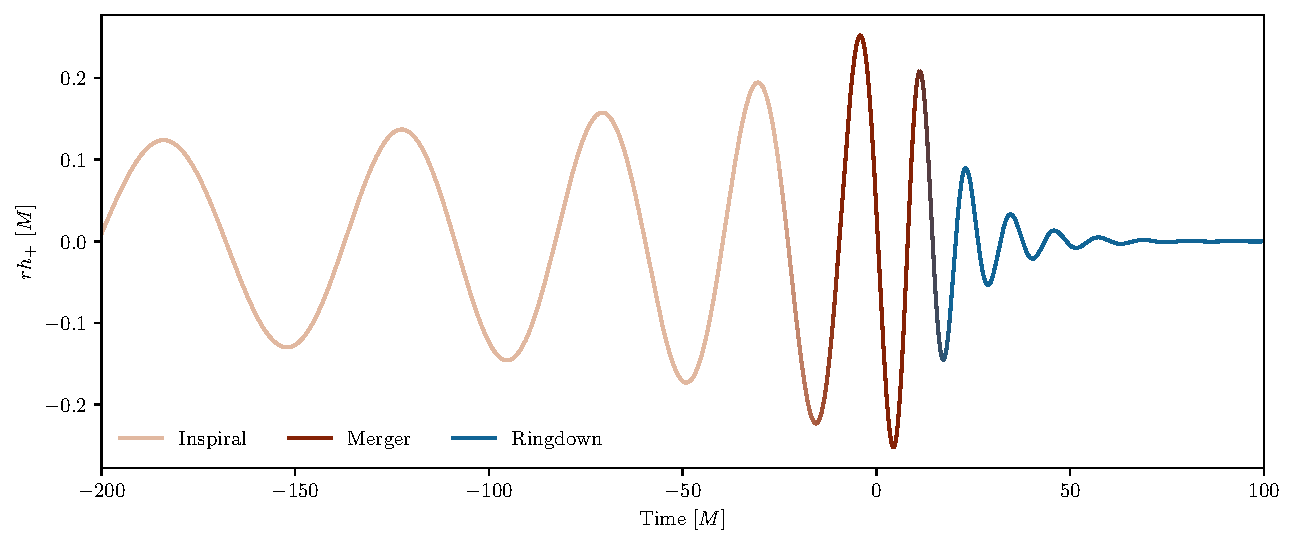
\includegraphics[width=\columnwidth]{Introduction/td_waveform.pdf}
    \caption[The time-domain gravitational-wave signal from a binary black-hole merger]{ 
    The GW signal from a BBH merger. 
    This waveform was generated using the NRSur7dq4 surrogate, and projected onto the Hanford detector using parameters consistent with GW150914 (this includes choosing a sky location and polarisation angle).
    }
    \label{ch1:fig:td_waveform}
\end{figure}

Going beyond these simple calculations, it is well-understood how the dynamics of compact-object mergers translate to the measured strain, which allows us to learn about the signal origin.
The GW signal from a BBH merger can be split into three stages: the inspiral, merger, and ringdown.
The inspiral corresponds to the two BHs in the binary orbiting each other. 
Unlike in the Newtonian case, the generation of GWs causes the system to lose energy (Eq.~\ref{ch1:eq:gw_luminosity}) and for the orbit to shrink and spiral. 
This stage in the binary evolution, where the motion of the orbit is slow compared to the speed of light, can be modelled with corrections to the Newtonian case in a post-Newtonian framework~\cite{Blanchet:2013haa}. 
Eventually, the BHs come together in the highly energetic and dynamical merger; this process requires the full nonlinear equations of GR, and is the subject of numerical relativity (NR)~\cite{Duez:2018jaf}. 
Immediately after merging, the final BH is highly distorted. 
As it equilibrates it produces GWs which roughly take the form of a damped sinusoid. 
This is analogous to the ringing a bell makes after it has been struck, and this final stage is called the ringdown.
Just as the early inspiral can be studied by considering deviations to a Newtonian system, the ringdown can be studied by considering perturbations to a static BH spacetime~\cite{Sasaki:2003xr, Pound:2021qin}. 
It is not known beforehand when this perturbative treatment of the final BH becomes valid (i.e., when the ringdown actually starts), and so care must be taken; this will be a recurring theme throughout this work.

The GW signal from these three stages is shown in Fig.~\ref{ch1:fig:td_waveform}.
Plotted is the (noiseless) GW strain signal projected onto the LIGO Hanford detector, $h$, multiplied by the distance to the source, $r$, as a function of time. 
We use geometric units ($G = c = 1$) to express these quantities in units of the total binary mass, $M$. 
In geometric units we can convert between lengths, masses, and times with appropriate combinations of $G$ and $c$; this means $\mathrm{time}/M$ and $rh/M$ can be made dimensionless quantities. 
Using GW150914 again as an example, say we had a system with total mass $M = 72\,M_\odot \approx 1.43 \times 10^{32}\,\mathrm{kg}$ at a distance $r = 440\,\mathrm{Mpc} \approx 1.36 \times 10^{25}\,\mathrm{m}$. 
Expressing $M$ in seconds gives us the conversion factor for time:
\begin{equation}
    M \times \frac{G}{c^3} \approx 1.43 \times 10^{32}\, \mathrm{kg} \times \frac{6.67 \times 10^{-11}\, \mathrm{m}^3\, \mathrm{kg}^{-1}\, \mathrm{s}^{-2}}{\qty(3 \times 10^8\, \mathrm{m}\, \mathrm{s}^{-1})^3} \approx 3.6 \times 10^{-4}\, \mathrm{s}.
\end{equation}
So, for these system properties, in Fig.~\ref{ch1:fig:td_waveform} we have a ringdown duration of $\sim 50\,M \approx 50 \times 3.6 \times 10^{-4}\,\mathrm{s} \approx 0.018\,\mathrm{s}$. 
Calculating the dimensionless quantity $M/r$ gives us the conversion for the GW amplitude. 
One way to do this is to express $r$ in seconds by dividing by $c$, then use our previous result for $M$:
\begin{equation}
    \frac{M \times G/c^3}{r/c} \approx \frac{3.6 \times 10^{-4}\,\mathrm{s}}{1.36 \times 10^{25}\, \mathrm{m}/3 \times 10^8\, \mathrm{m}\, \mathrm{s}^{-1}} \approx 7.85 \times 10^{-21}.
\end{equation}
This gives a peak strain amplitude in Fig.~\ref{ch1:fig:td_waveform} of $\sim 0.2 \times 7.85 \times 10^{-21} \approx 1.60 \times 10^{-21}$, in agreement with our order-of-magnitude calculation in Eq.~\ref{ch1:eq:quadrupole_strain_oom}. 
This can also be compared with what was actually measured for GW150914 (see Fig.~1 in Ref.~\cite{LIGOScientific:2016aoc}), and we see these numbers are consistent.

The waveform was generated using the NRSur7dq4~\cite{Varma:2019csw} surrogate waveform with zero spins, equal mass ratio, and zero inclination. 
Surrogates effectively ``interpolate'' the waveforms from full NR simulations, allowing quick waveform generation for any choice of system parameters (within the validity of the model). 
For NRSur7dq4, the simulations used to build the model came from the SXS catalog~\cite{Boyle:2019kee}, which we also use extensively in Chapter~\ref{Chapter2}. 
Along with the intrinsic system parameters, to project onto the Hanford detector we also choose an event time, sky location and polarisation angle consistent with GW150914.

\begin{figure}
    \centering
    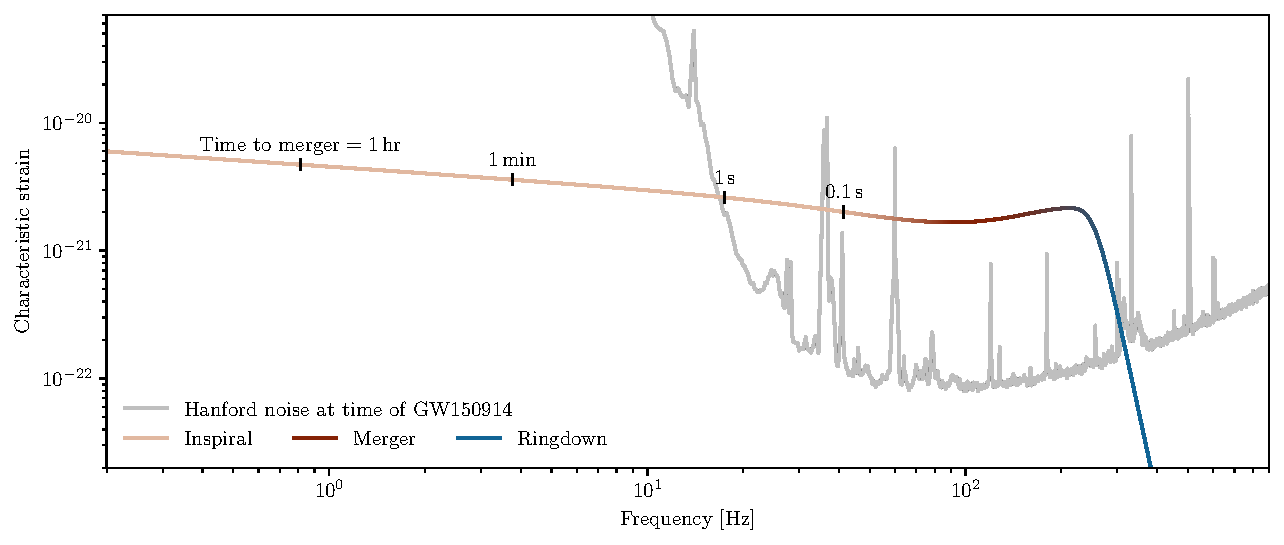
\includegraphics[width=\columnwidth]{Introduction/fd_waveform.pdf}
    \caption[The frequency-domain gravitational-wave signal from a binary black-hole merger]{ 
    The frequency-domain GW signal from a BBH merger, shown with the Hanford sensitivity curve (both expressed through the characteristic strain). 
    The signal was generated with IMRPhenomD using parameters consistent with GW150914.
    }
    \label{ch1:fig:fd_waveform}
\end{figure}

The above discussion disregards the sensitivity of the detector to different frequencies (i.e.\ the detector noise).
It is standard to treat the noise in the LIGO and Virgo detectors as stationary and Gaussian~\cite{LIGOScientific:2019hgc}.
Stationarity means that the noise covariance matrix is diagonal in the frequency domain (meaning there is no correlation between frequency bins), and so we can describe the noise with a power spectral density (PSD) $S_n(f)$.
In each frequency bin we model the noise as having a random phase and an amplitude drawn from a Gaussian distribution with standard deviation $\sqrt{S_n(f)}$.
We show the Hanford PSD in Fig.~\ref{ch1:fig:fd_waveform}, along with a frequency-domain BBH GW signal (both expressed through the characteristic strain, see Eqs.~\ref{ch1:eq:hn} and \ref{ch1:eq:hn}.
Since we are now comparing with a PSD, we fix the BBH total mass and distance to the example numbers used above ($M = 72\,M_\odot$, $r = 440\,\mathrm{Mpc}$).
Roughly speaking, the GW signal from a BBH merger increases in frequency over time.
The majority of the inspiral signal is at too low a frequency to be detected, with the GW signal only entering the detector band ($\sim 20$ to $\sim 1000\,\mathrm{Hz}$) just before merger.
Although the binary can spend millions of years inspiralling, we observe only the last few tenths of a second of the merger.
We choose to plot the signal and noise curve in terms of the characteristic strain~\cite{Moore:2014lga}, given by
\begin{equation}\label{ch1:eq:hc}
    h_c(f) = 2f\abs{\tilde{h}(f)}
\end{equation}
for the GW signal (where $\tilde{h}$ is the frequency-domain GW in a given detector), and
\begin{equation}\label{ch1:eq:hn}
    h_n(f) = \sqrt{fS_n(f)}
\end{equation}
for the noise curve.
The characteristic strain has the property that the area between the signal and noise curve is related to the signal-to-noise ratio (SNR) $\rho$ via
\begin{equation}
    \rho^2 = \int_{-\infty}^\infty \dd{\log{f}} \qty[\frac{h_c(f)}{h_n(f)}]^2.
\end{equation}
Evaluating for the above figure we get $\rho \sim 17$, which is consistent with the Hanford SNR for GW150914 (assuming equal SNRs in Hanford and Livingston, a network SNR of 26~\cite{LIGOScientific:2021usb} gives a single detector SNR of $\sim 18$).

Also shown in the figure is the time to merger at select frequencies of the inspiral.
This is to emphasise how the frequency of the binary evolves over time, spending the vast majority of its life in the inspiral with a slowly shrinking orbit.
The leading-order time to merger, $\tau_\mathrm{merge}$, as a function of GW frequency is given by
\begin{equation}\label{eq:time_to_merger}
    \tau_\mathrm{merge} = \frac{5}{256} \qty(\pi f)^{-\frac{8}{3}} \qty(\frac{G\mathcal{M}}{c^3})^{-\frac{5}{3}},
\end{equation}
% Give more details. Lowest order PN, what does it neglect? Valid for circular only...
% Say a bit about how it is derived.
where $\mathcal{M}$ is a combination of the two masses in the binary known as the chirp mass.
We also explicitly show the factors of $G$ and $c$ in this equation for clarity (in geometric units these would be set to 1, and it would be implied that the chirp mass should be expressed in units of time). 
Eq.~\ref{eq:time_to_merger} is valid in the quasi-circular orbit regime; it can be derived by equating the time derivative of the orbital energy of a binary system (

The signal in Fig.~\ref{ch1:fig:fd_waveform} was generated with the IMRPhenomD~\cite{Khan:2015jqa} waveform model, as implemented in the \texttt{ripple}~\cite{Edwards:2023sak} Python package.
Phenom models produce approximate waveforms using closed-form analytic expressions in the frequency-domain, making evaluation quick and suitable for GW searches.
The Hanford PSD is estimated from $1024\,\mathrm{s}$ of off-source data at the time of GW150914, using a Welch periodogram~\cite{1161901}.


\section{Black-hole ringdown}

The endpoint of a BBH, the ringdown signal is produced by the remnant BH settling to its stationary state.
Just as a bell or drum has a characteristic sound, so too does a BH; associated with the BH is a unique spectrum of oscillatory modes, determined purely by its properties (namely, for astrophysical BHs, a mass and spin).
The characteristic oscillations of the remnant BH are called quasinormal modes (QNMs), so-called because, unlike normal modes, they decay over time (for reviews on the subject, see Refs.~\cite{Kokkotas:1999bd, Nollert:1999ji, Ferrari:2007dd, Berti:2009kk}).
The QNM frequencies are complex, $\omega = 2\pi f - i/\tau$, with the real part $f$ giving the oscillation frequency and the reciprocal of the imaginary part $\tau$ giving the damping time. 
The QNM spectrum is the subject of Section~\ref{ch1:sec:qnms}.
The ringdown signal consists of a sum of QNMs, each excited a different amount depending on the initial configuration of the binary and how they merged; the excitation of different ringdown modes is among the areas of investigation in Chapter~\ref{Chapter2}.

\begin{figure}[ht!]
    \centering
    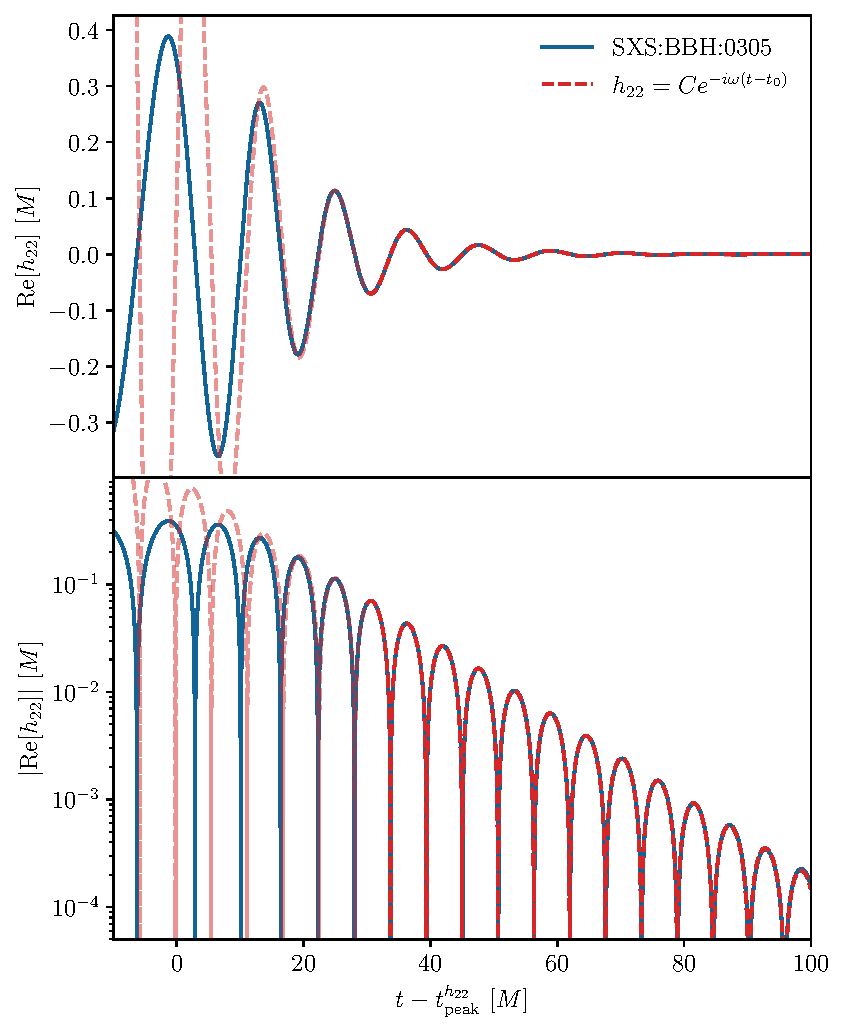
\includegraphics[width=\columnwidth]{Introduction/ringdown_waveform.pdf}
    \caption[The gravitational-wave ringdown signal]{ 
    The ringdown waveform from a BBH, fitted with a simple damped sinusoid. 
    At early times this simple description breaks down. The waveform is a NR simulation from the SXS catalog.
    }
    \label{ch1:fig:rd_waveform}
\end{figure}

Fig.~\ref{ch1:fig:rd_waveform} shows (in blue) the ringdown waveform from a NR simulation, SXS:BBH:0305~\cite{Lovelace:2016uwp}.
This simulation has properties consistent with GW150914, and will be among the NR simulations studied in Chapter~\ref{Chapter2}.
NR waveforms are decomposed into spherical-harmonic modes indexed by $\ell$ and $m$ (see Section~\ref{ch2:sec:model} and Eq.~\ref{ch2:eq:spherical_expansion} for more details), and here we plot the real part of the dominant $\ell = m = 2$ mode.
The radial dependence of GW waveforms goes predominantly as $r^{-1}$, so the SXS catalog provides the strain multiplied by $r$ (just as what was plotted in Fig.~\ref{ch1:fig:td_waveform}).
For clarity we will drop the $r$ factor for the remainder of the thesis and have the $r^{-1}$ scaling implied (just keep in mind when we refer to the GW signal $h$ or a mode $h_{\ell m}$, we really mean $rh$ and $rh_{\ell m}$). 

Overplotted is a simple model for the $h_{22}$ mode: a exponentially damped sinusoid with complex frequency $\omega = 2\pi f - i/\tau$ and amplitude $C = Ae^{i\phi}$. 
Taking the real part we have
\begin{align}
    \Re[Ce^{-i\omega(t-t_0)}] = A\cos[2\pi f(t-t_0) - \phi]e^{-(t-t_0)/\tau}.
\end{align}
That such a simple model describes the final stages of such a complicated system is a remarkable result, and is part of the power of studying the ringdown.
A faded red line traces the damped sinusoid to earlier times, where it starts to lose validity.
This is to be expected: at earlier times we approach the nonlinear and strong-gravity merger, where BH perturbation theory (which is where this linear description comes from) starts to break down.
Note, however, that our model here only includes a single term (i.e., one ringdown QNM); with additional QNMs we may be able to get a better fit to the NR waveform, or to describe the waveform at earlier times (this idea is explored at length in Chapter~\ref{Chapter2}).
A particular subset of QNMs, known as ``overtones'', will be of particular interest throughout the thesis; as well as featuring in the numerical studies of Chapter~\ref{Chapter2}, they will be a target in the analysis of GW data in Chapters~\ref{Chapter3} and \ref{Chapter4}.

A key goal in GW astronomy is the identification of QNMs in the ringdown signal.
We will see in the following sections that QNMs carry information about the remnant BH, meaning that measurements of QNM frequencies give us a way of inferring the remnant BH properties independently of the rest of the GW signal.
This forms the basis of important tests of GR, and is discussed further in Section~\ref{ch1:sec:bh_spectroscopy}.
The testing-GR companion papers for the second~\cite{LIGOScientific:2020tif} and third~\cite{LIGOScientific:2021sio} GW event catalogs featured searches for QNMs; of the detected events, results were reported for 22.
This can be taken as a rough guide for how many events have at least one measurable ringdown mode.
On top of this, tentative evidence was reported for the identification of an additional ringdown mode in a few of the loudest events, including GW150914.
However, as will be seen, the identification of subdominant ringdown modes is subtle.
This is particularly true for one of the most massive BBH mergers observed so far, GW190521~\cite{LIGOScientific:2020iuh}, which has a total source frame mass of $\sim 150\,M_\odot$.
Its large mass means this event enters the detector band only very near merger, and so is ringdown dominated.
This makes it a promising target for QNM searches, and along with GW150914 it is an event that will be referenced throughout this thesis. 

% GWTC-2: GW150914 and GW190521_074359 show some signs of an overtone. Mention contention re overtone? Probably best to save for later. 
% An event on the same day, known just as GW190521 CITE, is of particular interest to ringdown studies because of its exceptionally high mass. Not much inspiral... ringdown dominated... and analyses by others have claimed the identification of a higher harmonic.
% GWTC-3: GW200224_222234 shows log10B ~ 0.95 evidence for overtone

% If a system has a set of characteristic frequencies associated with it, then if we excite the system we can attempt to measure those frequencies and characterise the system. This is spectroscopy...

\section{Quasinormal modes}
\label{ch1:sec:qnms}

The characteristic vibrational modes of dissipative systems are known as QNMs.
As stated above, these differ from usual normal modes because they decay over time.
Although not limited to BHs (any real-world physical systems which are subject to damping will exhibit decaying modes), BH spacetimes are a unique case because even idealised systems are intrinsically dissipative. % ; this is due to the presence of the event horizon.

Gravitational perturbations of the Schwarzschild geometry~\cite{Schwarzschild:1916uq} were first studied by Regge and Wheeler~\cite{Regge:1957td}, and this work was extended by Zerilli to a more general class of perturbations~\cite{Zerilli:1970se, Zerilli:1970wzz}.
Employing the perturbation techniques developed by Regge and Wheeler, Vishveshwara~\cite{Vishveshwara:1970zz} performed numerical studies involving the scattering of GWs off a Schwarzschild BH.
It was found that the late-time GW waveform consisted of damped sinusoids, the form of which carried information about the BH mass. 
Further numerical work by Press~\cite{Press:1971wr}, studying the evolution of perturbations to the Schwarzschild geometry, identified the damped sinusoids as the ``free oscillation of a black hole''.
This work was also the first instance of the describing the vibration of a BH as a ``quasi-normal mode''.

Equations governing the perturbations of the Kerr metric~\cite{Kerr:1963ud} were found by Teukolsky~\cite{Teukolsky:1972my}. 
Describing rotating BHs, these are expected to be the most general class of astrophysical BH and will be the focus throughout this thesis. 
A remnant Kerr BH has ``no hair''~\cite{Carter:1971zc}; it is fully described by only a final mass and a an angular momentum (which we will express via a dimensionless spin parameter). 
The same is true of the spectrum of Kerr QNM frequencies, which are also functions of only the mass and spin. 
This is how QNMs carry information about the remnant BH, and this fact forms the basis of the GR tests discussed further in Section~\ref{ch1:sec:bh_spectroscopy}.

% In a normal-mode analysis, one usually has an ordinary differential equation, or a system of such equations, and imposes boundary conditions to the effect that the perturbation (or whatever wavefunction one is studying) must vanish outside a finite region in space. 
% An example of such a system is a finite string fixed at both ends, otherwise isolated from its surroundings. 
% This system is described by a self-adjoint operator with a discrete spectrum and a complete set of normal modes. 
% See Ref.~\cite{Berti:2006wq} for an interesting discussion, comparing the vibrating string problem to that of QNMs.
% Unfortunately, perturbations of black holes are quite different: the system we have is the metric outside the horizon in the case of a black hole.
% The perturbations will propagate throughout all space; we cannot demand that they should be zero outside a finite region. 
% Instead, we want to make sure that no gravitational radiation unrelated to the initial perturbation disturbs the system at late times.

The QNM frequencies can be calculated within the framework of linearised gravity, treating the gravitational field in the vicinity of the remnant as a small (linear) perturbation of the Kerr metric.
Therefore, the QNM description of the GW signal is only expected to be valid at sufficiently late times, when the nonlinearities from the merger have largely decayed away. 
In the following subsections we discuss the calculation and physical picture of QNMs further to help build some intuition.

% QNMs also have practical uses in waveform modelling. 
% They are used in full inspiral-merger-ringdown BBH waveforms produced in both the phenomenological \cite{Pratten:2020ceb, Garcia-Quiros:2020qpx, Pratten:2020fqn} and effective-one-body approaches \cite{Buonanno:2006ui, Buonanno:2007pf, Pan:2011gk}.

\subsection{Scalar field on a Schwarzschild background}

To help build some intuition regarding the origin of the QNMs, we will perform a demonstrative calculation involving a massless scalar field, $\psi(t,r,\theta,\phi)$ on a Schwarzschild background.
This will lead to equations reminiscent of the Zerilli and Regge-Wheeler equations, without the complication of tensor spherical harmonics that comes with the full gravitational-perturbation treatment.

The metric tensor, in Schwarzschild coordinates, is
\begin{equation}
g_{\mu\nu} = \begin{pmatrix}
- \left(1 - \frac{2M}{r}\right) & 0 & 0 & 0 \\
0 & \left(1 - \frac{2M}{r}\right)^{-1} & 0 & 0 \\
0 & 0 & r^2 & 0 \\
0 & 0 & 0 & r^2 \sin^2\theta
\end{pmatrix},
\end{equation}
where now $M$ is the mass of the BH (and not the total mass of the binary, as before). 
The relevant massless wave equation, qualitatively similar to equations describing GWs and electromagnetic waves (and used here as a toy model for the GW perturbations of a BH), is the Klein-Gordon equation 
\begin{equation}
    \nabla_\mu \nabla^\mu \psi = 0.
\end{equation}
Using the fact that a covariant derivative reduces to the partial derivative on scalars, we can write this as
\begin{equation}
    \nabla_\mu \nabla^\mu \psi = \frac{1}{\sqrt{-g}} \partial_\mu \qty(\sqrt{-g} g^{\mu\nu} \partial_\nu \psi) = 0
\end{equation}
where $g$ is the determinant of the metric tensor, $g^{\mu\nu}$ is the inverse of the metric tensor, and we have also used $\Gamma^\mu_{\mu\nu} = \partial_\nu \ln{\sqrt{-g}} = \qty(-g)^{-1/2} \partial_\nu \sqrt{-g}$.
For Schwarzschild we have $\sqrt{-g} = r^2 \sin{\theta}$.
Evaluating, we get
\begin{multline}
    - \qty(1 - \frac{2M}{r})^{-1} \pdv[2]{\psi}{t} + \frac{1}{r^2} \pdv{r} \qty[r^2 \qty(1 - \frac{2M}{r}) \pdv{\psi}{r} ]\\
    + \frac{1}{r^2} \qty[ \frac{1}{\sin{\theta}} \pdv{\theta} \qty(\sin{\theta} \pdv{\psi}{\theta} ) + \frac{1}{\sin^2{\theta}} \pdv[2]{\psi}{\phi} ] = 0.
\end{multline}
Recognising that the scalar spherical harmonics, $Y_{\ell m}(\theta,\phi)$, are the eigenfunctions of the angular part:
\begin{equation}
    \frac{1}{\sin{\theta}} \pdv{\theta} \qty(\sin{\theta} \pdv{Y_{\ell m}}{\theta} ) + \frac{1}{\sin^2{\theta}} \pdv[2]{Y_{\ell m}}{\phi} = - \ell (\ell + 1) Y_{\ell m},
\end{equation}
we will attempt a spherical harmonic decomposition of the scalar field. 
With the expectation that the radial dependence of the field will go as $1/r$ (and also anticipating a change in radial coordinate) we write the scalar field as
\begin{equation}
    \psi(t, r, \theta, \phi) = \frac{1}{r} \sum_{\ell = 0}^\infty \sum_{m = -\ell}^\ell \psi_{\ell m}(t, r) Y_{\ell m}(\theta, \phi).
\end{equation}
Note that here, in the scalar case, the sum over $\ell$ starts from $\ell = 0$.
In general, the sum will start from $\ell = \abs{s}$, where $s$ is the spin weight of the field ($s=0$, $-1$ and $-2$ for scalar, electrical, and gravitational perturbations respectively).
Substituting, we are left with an equation for the radial part:
\begin{multline}
    - \pdv[2]{\psi_{\ell m}}{t} + \frac{1}{r} \qty(1 - \frac{2M}{r}) \pdv{r} \qty[r^2 \qty(1 - \frac{2M}{r}) \pdv{r}\qty(\frac{\psi_{\ell m}}{r}) ]\\
    - \qty(1 - \frac{2M}{r}) \qty(\frac{\ell (\ell + 1)}{r^2}) \psi_{\ell m} = 0.
\end{multline}
To proceed we introduce the tortoise coordinate, $r_*$,
\begin{equation}
    r_* = r + 2M \ln(\frac{r}{2M} - 1),
\end{equation}
which has the property that
\begin{equation}
    \dv{r_*}{r} = \qty( 1 - \frac{2M}{r} )^{-1}.
\end{equation}
Note that as $r$ approaches the Schwarzschild radius ($r \rightarrow 2M$), the tortoise coordinate $r_* \rightarrow -\infty$.
Making this change of variables, we arrive at
\begin{equation}\label{eq:wave_equation}
    \pdv[2]{\psi_{\ell m}(t,r)}{r_*} - \pdv[2]{\psi_{\ell m}(t,r)}{t} - V_\ell(r) \psi_{\ell m}(t,r) = 0,
\end{equation}
where
\begin{equation}
    V_\ell(r) = \qty( 1 - \frac{2M}{r} ) \qty( \frac{\ell (\ell + 1)}{r^2} + \frac{2M}{r^3} )
\end{equation}
is an effective potential.
Performing a Fourier transform, 
\begin{equation}\label{ch1:eq:ft}
    \tilde{\psi}_{\ell m}(\omega,r) = \int_{-\infty}^\infty \dd{t} \psi(t,r) e^{-2\pi i f t},
\end{equation}
we can bring Eq.~\ref{eq:wave_equation} into the form of a one-dimensional Schr\"{o}dinger equation
\begin{equation}\label{eq:fd_wave_equation}
    \pdv[2]{\tilde{\psi}_{\ell m}(\omega,r)}{r_*} + \qty[ \omega^2 - V_\ell(r)] \tilde{\psi}_{\ell m}(\omega,r) = 0.
\end{equation}
Gravitational perturbations obey an equation of the same form (i.e. the Regge-Wheeler and Zerilli equations), and in fact the effective potential can be written in the unified form
\begin{equation}
    V_\ell(r) = \qty( 1 - \frac{2M}{r} ) \qty( \frac{\ell (\ell + 1)}{r^2} + \frac{(1 - s^2)2M}{r^3} )
\end{equation}
with $s = 0$, $-1$ and $-2$ for scalar, electrical, and gravitational perturbations respectively. 
The effective potential in the Zerilli equation has a slightly different form (the Zerilli equation describes polar, or even-parity, perturbations, whereas the Regge-Wheeler equations describes axial, or odd-parity, perturbations). 
However, it has been shown that the QNM spectrum resulting from the Regge-Wheeler and Zerilli equations are identical~\cite{Chandrasekhar:1975nkd}.

\begin{figure}[t]
    \centering
    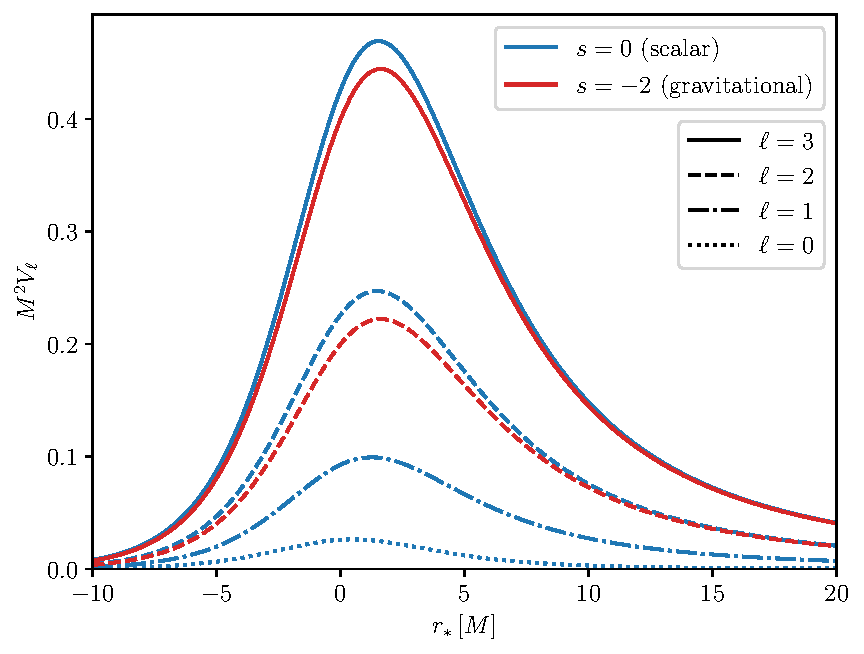
\includegraphics[width=0.8\columnwidth]{Figures/Introduction/rw_potential.pdf}
    \caption[The Regge-Wheeler potential]{
    The Regge-Wheeler potential as a function of the tortoise coordinate $r_*$ (with the BH horizon at $r_* = -\infty$), for scalar and gravitational perturbations and for a selection of $\ell$. In this subsection $M$ refers to the mass of the Schwarzschild BH, and not the total binary mass.
    }
    \label{fig:rw_potential}
\end{figure}

We must specify boundary conditions to find the QNM solutions.
When solving for the normal modes on a string, or the energy levels of a quantum harmonic oscillator, we require the wavefunction to vanish at the boundaries (either at the string ends, or at $\pm \infty$ for the harmonic oscillator).
The problem we're considering here is slightly different; the potential, depicted in Fig.~\ref{fig:rw_potential}, clearly does not admit bound states. 
It does not have a minima, and $V_\ell(r) > 0$ for all $r$.
The implication is that we should look for plane wave solutions that are ingoing to the BH horizon, and outgoing to infinity:
\begin{alignat}{2}
    &\tilde{\psi}_{\ell m}(\omega, r) \sim e^{i \omega r_*} \qquad &&\qty(r_* \rightarrow -\infty) \nonumber \\
    &\tilde{\psi}_{\ell m}(\omega, r) \sim e^{- i \omega r_*} \qquad &&\qty(r_* \rightarrow \infty).
\end{alignat}
This follows from the consideration that the field should radiate only inward at the horizon and only outward at spatial infinity.

This gives us a well-posed problem, and now all that is left is the computation of the QNMs. 
A variety of methods have been used~\cite{Kokkotas:1999bd, Berti:2004md}, with the first attempts consisting of the aforementioned time-domain evolutions of the Regge-Wheeler and Zerilli equations by Vishveshwara~\cite{Vishveshwara:1970zz} and Press~\cite{Press:1971wr}. 
In principle the QNM frequencies can be extracted from the resulting waveform, but this approach does not return the complete spectrum (in practice only a subset of modes can be extracted).
Chandrasekhar and Detweiler~\cite{Chandrasekhar:1975zza} employed a shooting method to directly integrate the wave equation in the frequency domain; this involves picking a value for the QNM frequency, integrating, and checking whether the boundary conditions are satisfied. 
This is an inefficient way of identifying QNMs, and this approach is also prone to numerical noise.
Analytical methods were developed by Blome, Mashhoon and Ferrari~\cite{BLOME1984231, Ferrari:1984ozr, Ferrari:1984zz}, which consider the bound states of the inverted BH potential. 
Although not in general accurate, this approach offers physical insight which we touch upon in the next subsection.
Motivated by the analogy between Eq.~\ref{eq:wave_equation} and the Schr\"{o}dinger equation, Schutz and Will~\cite{Schutz:1985km} employed WKB methods to calculate a handful of fundamental mode QNM frequencies.
This approach has since been improved upon~\cite{Iyer:1986np, Matyjasek:2017psv, Konoplya:2019hlu}, 
% Iyer:1986nq, Kokkotas:1988fm, Seidel:1989bp, Kokkotas:1991vz, Konoplya:2003ii, 
and can give very accurate results for certain modes (but, again, breaks down in some limits). 
Finally, a numerical method utilising continued fractions (proposed by Leaver~\cite{Leaver:1985ax}, and later improved upon by Nollert~\cite{Nollert:1993zz}) is known to be highly accurate and fast.
It is the method of choice in modern codes such as the \texttt{qnm} Python package~\cite{Stein:2019mop} (which is used in work throughout this thesis).

In summary, when enforcing the above boundary conditions, only discrete values of $\omega$ satisfy Eq.~\ref{eq:fd_wave_equation}; these are the QNMs.
In the case of a Kerr BH, we denote the QNMs $\omega_{\ell m n}$.
They are indexed by three numbers: the usual angular indices $\ell$ and $m$, and an additional ``overtone'' index $n$.
We present the solutions in Section~\ref{ch1:sec:bh_spectroscopy} and in Fig.~\ref{ch1:fig:qnm_taxonomy}.
The full computation of the spectrum is beyond the scope of this work.
We instead consider a simple calculation of QNMs using the geodesic correspondence in order to build some physical intuition.

\subsection{Quasinormal modes from the geodesic correspondence}

First pointed out by Goebel~\cite{1972ApJ...172L..95G}, there exists a relation between BH QNMs and null geodesics around the BH spacetime.
Having since been developed further~\cite{BLOME1984231, Ferrari:1984ozr, Ferrari:1984zz, Cardoso:2008bp, Yang:2012he}, this approach provides a physical insight to QNMs; that is, QNMs can be interpreted as GWs slowly leaking out of a light-ring orbit around the BH. 
Although only valid for $\ell \gg 1$ (known as the eikonal, or geometrical optics, limit), this correspondence greatly simplifies the calculations of QNMs since it only depends on the background metric.
Consequently, it offers a way to compute QNMs in beyond GR theories (for example, as was done in Ref.~\cite{Blazquez-Salcedo:2016enn}), or for computing the QNM spectrum for charged (Kerr-Newman~\cite{Newman:1965my}) BHs~\cite{Cardoso:2016olt, Wang:2021uuh} which can be challenginf with the previously discussed methods (but, see also Ref.~\cite{Carullo:2021oxn} where a more sophisticated analysis was done).

The key result is that the QNM frequencies for a Kerr BH in the eikonal limit can be written as
\begin{equation}\label{ch1:eq:eikonalomega}
    \omega_{\ell m n} = 2\pi f_{\ell m n} - \frac{i}{\tau_{\ell m n}} = \qty(\ell + \frac{1}{2}) \Omega_\theta + m \Omega_\mathrm{pre} - i \qty(n + \frac{1}{2}) \gamma_L.
\end{equation}
Here, $\Omega_\theta$ is the frequency of small oscillations in the polar direction of a perturbed geodesic. 
The precessional frequency of the orbital plane, $\Omega_\mathrm{pre}$, is given by $\Omega_\mathrm{pre} = \Omega_\phi - \Omega_\theta$, where $\Omega_\phi$ is the orbital frequency of the light ring.
Finally, $\gamma_L$ is the Lyapunov exponent of the light ring; this can be thought of as a measure of the stability of the orbit.
More precisely, it characterises the rate at which the cross section of a congruence of null geodesics on the circular photon orbit increases under radial perturbations.
Crucially, these quantities are all determined by the metric. 
Below we take a the case of a stationary and axisymmetric spacetime (i.e.\ the spacetime associated with a rotating BH) and show how one can calculate the relevant quantities.
For this demonstrative calculation we set $\ell = m$, associated with prograde equatorial motion, to simplify the calculations.
Note that, with the assumption $\ell = m \gg 1$, we can write the real part of the QNM frequency as
\begin{equation}
    \qty(\ell + \frac{1}{2}) \Omega_\theta + m \Omega_\mathrm{pre} \sim \ell \Omega_\theta + \ell \qty(\Omega_\phi - \Omega_\theta) = \ell \Omega_\phi,
\end{equation}
which aligns with the interpretation of QNMs originating as GWs in light ring orbits.

First, we need the metric associated with a stationary and axisymmetric spacetime. 
The stationary and axisymmetric character requires that the metric coefficients be independent of $t$ and $\phi$, so that $g_{\mu \nu} = g_{\mu \nu}(r,\theta)$. 
Note that we haven't imposed equatorial motion ($\theta = \pi/2$) yet.
We also require that the spacetime is invariant to the simultaneous inversion of the time $t$ and the angle $\phi$ (i.e.\ to the transformation $t \rightarrow -t$, $\phi \rightarrow -\phi$). 
This has the physical meaning that the spacetime we are considering is associated with a rotating body. 
This invariance requires 
\begin{equation}
	g_{tr} = g_{t \theta} = g_{\phi r} = g_{\phi \theta} = 0.
\end{equation}
Then we have 
\begin{equation}
	\dd s^2 = g_{tt}\dd t^2 + 2g_{t \phi} \dd t \dd \phi + g_{\phi \phi}\dd \phi^2 + \qty[ g_{rr}\dd r^2 + 2g_{r \theta} \dd r \dd \theta + g_{\theta \theta} \dd \theta^2 ].
\end{equation}
It can be shown~\cite{Chandrasekhar:1985kt} that the term in square brackets can be brought to the diagonal form $g_{r'r'}\dd r'^2 +  g_{\theta' \theta'} \dd \theta'^2$ by a change of coordinates $r'=r'(r,\theta)$ and $\theta'=\theta'(r,\theta)$.
Renaming our variables by removing the primes, this gives
\begin{equation}
	\dd s^2 = g_{tt}\dd t^2 + g_{rr}\dd r^2 + g_{\theta \theta}\dd \theta^2 + g_{\phi \phi}\dd \phi^2 + 2g_{t \phi}\dd t\dd \phi.
\end{equation}
We can find geodesic curves $x^\mu(\lambda)$ by extremising the action $S=\int\mathrm{d}\lambda\,\mathcal{L}$ where the Lagrangian is given by
\begin{align}
	\mathcal{L} &= \frac{1}{2}g_{\mu \nu} \dot{x}^\mu \dot{x}^\nu \\
	&= \frac{1}{2}\qty(g_{tt}\dot{t}^2 + g_{rr}\dot{r}^2 + g_{\theta \theta}\dot{\theta}^2 + g_{\phi \phi}\dot{\phi}^2 + 2g_{t \phi}\dot{t}\dot{\phi}), \nonumber
\end{align}
and a dot denotes a derivative with respect to the affine parameter $\lambda$ along the curve. 
We proceed with the Euler-Lagrange (EL) equations, 
\begin{gather} \label{eq:ELeqns_1}
	\dv{\lambda}(\pdv{\mathcal{L}}{\dot{x}^\mu}) = \pdv{\mathcal{L}}{x^\mu}.
\end{gather}
Firstly, the stationarity of our spacetime leads to a constant of motion (the energy):
\begin{equation}\label{eq:el_t} 
	\pdv{\mathcal{L}}{\dot{t}} = -E \implies g_{tt}\dot{t} + g_{t\phi}\dot{\phi} = -E.
\end{equation}
Similarly, from the axisymmetry of the spacetime we have a second constant of motion (the angular momentum):
\begin{equation}\label{eq:el_phi}
	\pdv{\mathcal{L}}{\dot{\phi}} =L \implies g_{\phi \phi}\dot{\phi} + g_{t\phi}\dot{t} = L.
\end{equation}
From Eqs.~\ref{eq:el_t} and \ref{eq:el_phi} we can solve for the two components of the four-velocity $\dot{t}$ and $\dot{\phi}$ to give
\begin{gather} \label{eq:tdot_L}
	\dot{t} = E \frac{g_{\phi \phi} + g_{t \phi}\hat{L}}{\qty(g_{t \phi})^2 - g_{t t}g_{\phi \phi}} \\
	\label{eq:phidot_L}
	\dot{\phi} = E \frac{g_{t \phi} + g_{t t}\hat{L}}{g_{t t}g_{\phi \phi} - \qty(g_{t \phi})^2}
\end{gather}
where $\hat{L} = L/E$ is the specific angular momentum.
We are also free to rescale our affine parameter $\lambda\rightarrow E\lambda$ to remove $E$ from the above expressions.
Using the above, the azimuthal orbital frequency can be calculated:
\begin{gather}
	\Omega_\phi = \frac{\mathrm{d}\phi}{\mathrm{d}t} =  \frac{\dot{\phi}}{\dot{t}} = -\frac{g_{t\phi}+g_{tt}\hat{L}}{g_{\phi\phi}+g_{t\phi}\hat{L}}.
\end{gather}
In general, for the remaining two coordinates ($r$ and $\theta$) we can use the EL equations to find the second-order differential geodesic equations.
However, now we impose the simplification of equatorial motion mentioned previously: $\theta=\pi/2$.
This implies $\dot{\theta}=0$ in the case of reflective symmetry about the equator. 
This allows us to get a first order equation for $\dot{r}$ by considering the four-velocity for null geodesics:
\begin{equation} \label{eq:rdot}
	g_{\mu\nu}\dot{x}^\mu\dot{x}^\mu = 0 \implies \dot{r}^2 = V_{\rm eff}(r;\hat{L}),
\end{equation}
where
\begin{align}\label{eq:Veff}
	V_{\rm eff}(r;\hat{L}) &= \frac{-g_{tt}\dot{t}^2 -g_{\phi\phi}\dot{\phi}^2-2g_{t\phi}\dot{t}\dot{\phi} }{g_{rr}} \nonumber \\
	&= \frac{g_{tt} \hat{L}^2+2 g_{t\phi } \hat{L}+g_{\phi\phi}}{g_{rr}(g_{t\phi}^2-g_{tt} g_{\phi \phi})},
\end{align}
and in the final line we have used Eqs.~\ref{eq:tdot_L} and \ref{eq:phidot_L} to eliminate $\dot{t}$ and $\dot{\phi}$.
In Eq.~\ref{eq:Veff} the $g_{\mu\nu}$ metric coefficients are to be evaluated on the equatorial plane $\theta=\pi/2$ and so are only functions of $r$.
A light ring is a circular null geodesic orbit. 
The radius, $r_*$, and angular momentum, $\hat{L}_*$, of such an orbit must satisfy $V_{\rm eff} = V'_{\rm eff} = 0$, where a prime denotes a radial derivative with respect to $r$. The first condition yields
\begin{equation}
	\hat{L}_*(r) = \frac{-g_{t \phi} \pm \sqrt{g_{t \phi}^2 - g_{t t}g_{\phi \phi}}}{g_{t t}},
\end{equation}
while the second gives an implicit formula for $r_*$:
\begin{equation}\label{ch1:eq:veffprime}
	V'_{\rm eff}\big(r_*;\hat{L}_*(r_*)\big) = 0.
\end{equation}
In general we solve Eq.~\ref{ch1:eq:veffprime} numerically to obtain the light ring radius.
For prograde equatorial orbits in the Kerr metric this will have a single root, but will depend on the spin chosen for the spacetime.

Having found the equations of the light ring, we now consider neighbouring geodesics (i.e.\ perturbations to the light ring) to determine $\Omega_\theta$ and the Lyapunov exponent. 
First, consider polar motion. 
The EL equation for $\theta$ is 
\begin{multline}\label{eq:el_theta}
	g_{\theta \theta} \ddot{\theta} + \qty(\pdv{g_{\theta \theta}}{\theta} \dot{\theta} + \pdv{g_{\theta \theta}}{r} \dot{r}) \dot{\theta} \\
	= \frac{1}{2} \bigg(\pdv{g_{t t}}{\theta} \dot{t}^2 + \pdv{g_{r r}}{\theta} \dot{r}^2 + \pdv{g_{\theta \theta}}{\theta} \dot{\theta}^2 + \pdv{g_{\phi \phi}}{\theta} \dot{\phi}^2 + 2\pdv{g_{t \phi}}{\theta} \dot{t}\dot{\phi}\bigg).
\end{multline}
We consider small perturbations in the $\theta$ direction about the light ring.
That is, we set $r = r_*$ and $\theta = \pi/2+\delta\theta$.
Discarding terms $\mathcal{O}(\delta\theta^2)$ (and with $\dot{t}$ and $\dot{\phi}$ given by Eqs.~\ref{eq:tdot_L} and \ref{eq:phidot_L} respectively) we obtain
\begin{multline}\label{eq:el_theta_expanded}
	g_{\theta \theta}(r_*,\pi/2) \delta\ddot{\theta} \\
 = \frac{1}{2} \bigg(\pdv[2]{g_{t t}(r_*,\pi/2)}{\theta} \dot{t}^2 + \pdv[2]{g_{\phi\phi}(r_*,\pi/2)}{\theta} \dot{\phi}^2 + 2\pdv[2]{g_{t \phi}(r_*,\pi/2)}{\theta} \dot{t}\dot{\phi}\bigg)\delta\theta.
\end{multline}
which describes simple harmonic motion, $\delta\ddot{\theta} = -\tilde{\Omega}^2_\theta \delta\theta$, where the constant $\tilde{\Omega}_\theta$ is the frequency of the oscillations with respect to the parameter $\lambda$.
The frequency of the oscillations with respect to coordinate time $t$ is given by
\begin{align}
    \Omega_\theta = \frac{\tilde{\Omega}_\theta}{\dot{t}} &= \frac{1}{\dot{t}} \sqrt{-\frac{1}{2g_{\theta\theta}}\qty(\pdv[2]{g_{tt}}{\theta}\dot{t}^2 + 2\pdv[2]{g_{t\phi}}{\theta}\dot{t}\dot{\phi} + \pdv[2]{g_{\phi\phi}}{\theta}\dot{\phi}^2)} \nonumber \\
    &= \sqrt{-\frac{1}{2g_{\theta\theta}}\qty(\pdv[2]{g_{tt}}{\theta} + 2\pdv[2]{g_{t\phi}}{\theta}\Omega_\phi + \pdv[2]{g_{\phi\phi}}{\theta}\Omega_\phi^2)},
\end{align}
where all quantities on the right hand side are to be evaluated at the light ring. 
In the case of the Kerr metric $\Omega_\theta^2 > 0$ and the light ring is stable in the polar direction.

Now consider motion in the radial direction ($\dot{r} \neq 0$).
Differentiating Eq.~\ref{eq:rdot} with respect to $\lambda$ gives
\begin{equation}
	\ddot{r} = \frac{1}{2} \frac{\dot{V}_\mathrm{eff}(r)}{\dot{r}} = \frac{1}{2}V'_\mathrm{eff}(r).
\end{equation}
Consider small perturbations $r = r_* + \delta r$ with $\theta = \pi/2$ and discarding $\mathcal{O}(\delta r^2)$ terms gives
\begin{equation}
	\delta \ddot{r} = \frac{1}{2}V''_{\rm eff}(r_*)\delta r.
\end{equation}
Looking for periodic solutions, the frequency of the radial oscillations (with respect to coordinate time) is given by
\begin{align}
	\Omega_{r} = \sqrt{-\frac{V''_{\rm eff}(r_*)}{2\dot{t}^2}}.
\end{align}
In the case of the Kerr metric the light ring orbit has $\Omega_r^2 < 0$ and is unstable in the radial direction; we can define the Lyapunov exponent as
\begin{equation}
    \gamma_L = -i\Omega_r = \sqrt{\frac{V''_\mathrm{eff}(r_*)}{2\dot{t}}}
\end{equation}
and the corresponding decay timescale from Eq.~\ref{ch1:eq:eikonalomega} is
\begin{equation}
    \tau_{\ell m n} = \qty(n + \frac{1}{2})^{-1} \sqrt{\frac{2\dot{t}^2}{V''_\mathrm{eff}(r_*)}}.
\end{equation}
We conclude this section with a discussion of some the problems associated with QNMs.
In Section~\ref{ch1:sec:bh_spectroscopy} we will discuss the full (and accurately computed) QNM spectrum further, and the tests of GR that can be done with the observation of QNMs.

\subsection{Limitations of quasinormal modes}
\label{ch1:sec:limitations}

Although QNMs offer a powerful tool to learn about the remnant BH and test our theories (see Section~\ref{ch1:sec:bh_spectroscopy}), there are some subtleties regarding the QNM spectrum and the ringdown signal that should be pointed out. 

It is known that QNMs do not form a complete basis~\cite{Ching:1993gt, Ching:1995rt, Nollert:1998ys, Ching:1998mxl, Nollert:1999ji}, meaning that there are other contributions to the ringdown waveform beyond the QNMs.
In particular, it is known that at late times the ringdown consists of a power-law tail~\cite{Price:1971fb, Leaver:1986gd, Ching:1995tj} (see also Ref.~\cite{Gleiser:2007ti}, and references therein, for a more recent discussion about our knowledge of tails).
Although at a much lower amplitude than the QNM ringing and not resolvable at current detector sensitivities, at sufficient SNRs these may need to be considered to avoid biases.
This idea was touched upon in Ref.~\cite{Thrane:2017lqn}, where it was found that their ability to constrain remnant parameters from the ringdown signal actually degraded at high SNRs (late-time tails were suggested as an explanation for this, but it is not clear if they were responsible in this study).
% See also Ref.~\cite{Nee:2023osy}, who point out that the tendency for their QNM fits to perform worse at late times is a sign of tails.
See also Ref.~\cite{Baibhav:2017jhs} for a study on how neglecting these beyond-QNM contributions could bias future studies.

Motivated by work done in Refs.~\cite{Ching:1993gt, Ching:1995rt}, Nollert~\cite{Nollert:1996rf} attempted to make the QNM spectrum complete via modifications to the effective potential (for example, in the case of Schwarzschild, the Regge-Wheeler potential depicted in Fig.~\ref{fig:rw_potential}).
However, it was found that the QNM spectrum is highly unstable to changes in the potential (no matter how small).
That is, perturbations to the potential (which do not significantly change the physical ringdown waveform) can lead to very different QNM spectra; this brings the physical meaning of the QNMs into question.
This fact was commented on again in Nollert and Price~\cite{Nollert:1998ys}, later revisited by Daghigh et al.~\cite{Daghigh:2020jyk}, and additional recent work is ongoing~\cite{Jaramillo:2020tuu, Qian:2020cnz, Jaramillo:2021tmt, Cheung:2021bol, Berti:2022xfj}.

Putting these subtleties aside, we know we can calculate the QNM spectrum (as described throughout this section, and see Fig.~\ref{ch1:fig:qnm_taxonomy} below) and based on the GW observations made so far it seems that there is physical significance to the QNMs.
However, the excitations of each mode (that is, the amplitudes of each QNM in the ringdown waveform) are harder to predict. 
In principle the QNM amplitudes are a function of the initial conditions of the binary; the perturbation of the remnant BH depends on the way the binary merged.
Unfortunately this mapping is non-trivial, particularly in the case of precessing BBHs.
The QNMs we include in our models and target in the data must then be motivated by numerical studies.
We contribute to this in Chapter~\ref{Chapter2}, where we also discuss this issue in more detail.

Similarly to the mode amplitudes, a priori it is not known what the start time of the ringdown is.
Even with clean, noise-free numerical simulations it is not clear if the start time can be determined unambiguously.
This is an issue which will be present throughout the thesis, and in the data-analysis context (Chapters~\ref{Chapter3} and \ref{Chapter4}) we propose a method to alleviate this concern.

Finally, on the subject of data analysis, the fact that ringdown models are fundamentally discontinuous leads to data analysis problems; GW analysis is usually done in the frequency domain, but Fourier transforms of a discontinuous model leads to spectral leakage.
This is discussed further in Chapters~\ref{Chapter3} and \ref{Chapter4}, where we also propose a solution.

\section{Black-hole spectroscopy}
\label{ch1:sec:bh_spectroscopy}

The full Kerr QNM spectrum is nowadays readily available, with modern codes (such as the \texttt{qnm} package~\cite{Stein:2019mop}) making use of a version of Leaver's method~\cite{Leaver:1985ax} to compute them accurately and quickly.
We show the $\ell = 2$, $n = 0$; $\ell = 3$, $n = 0$; and $\ell = 2$, $n = 1$ branches of the Kerr spectrum in Fig.~\ref{ch1:fig:qnm_taxonomy} (of course, the full spectrum would extend to infinity in both $\ell$ and $n$, but the branches shown here include the QNMs expected to be of most interest at current detector sensitivities).  

There are different conventions used in the literature to label the modes; we aim to clarify these with Fig.~\ref{ch1:fig:qnm_taxonomy}.
Firstly, we see the QNMs appear to come in pairs: those with positive real part, and those with negative real part.
These are the ``regular'' and ``mirror'' (sometimes called ``twin'' or ``conjugate'') QNMs respectively.
Denoting the mirror QNM frequency with a prime, we can relate $\omega'_{\ell m n}$ to the regular QNMs as follows~\cite{Berti:2005ys}:
\begin{equation}
    f'_{\ell m n} = -f_{\ell -m n}, \quad \tau'_{\ell m n} = \tau_{\ell -m n} \nonumber
\end{equation}
\begin{equation} 
    \quad\Rightarrow\quad \omega'_{\ell m n} = - \omega_{\ell -mn}^*.
    \label{ch1:eq:mirror}
\end{equation}
So, for example, when we refer to the ``$(2,-2,0)$ mirror mode'', we are referring to the mode that is the ``mirror image'' of the regular $(2,2,0)$ mode in Fig.~\ref{ch1:fig:qnm_taxonomy}.
This way of referring to the modes allows us to unambiguously refer to every mode in the spectrum, including the $m=0$ modes, and will be the preferred method in this work.

\begin{figure}[t]
    \centering
    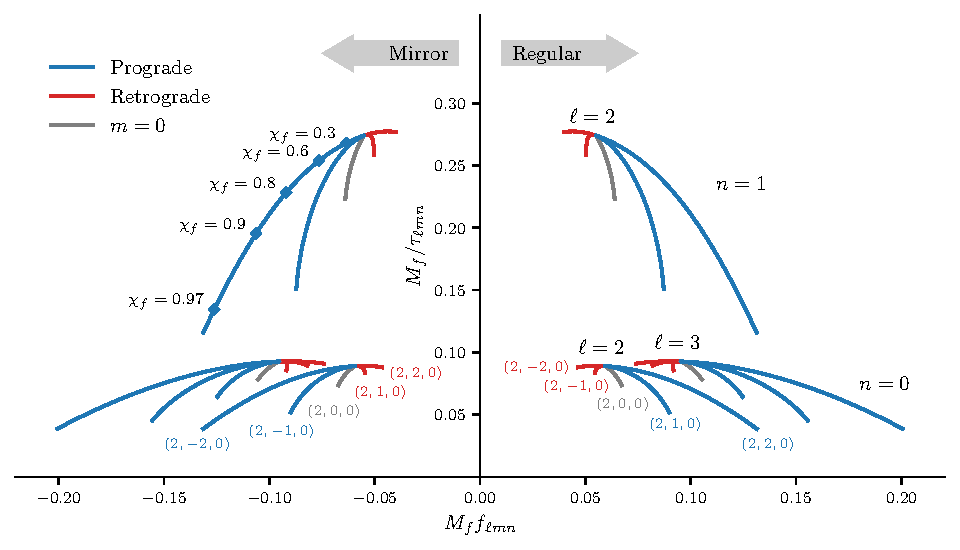
\includegraphics[width=\columnwidth]{Introduction/qnm_taxonomy.pdf}
    \caption[The Kerr quasinormal mode spectrum]{ 
    Selected modes of the Kerr QNM spectrum. BH QNM frequencies are conventionally represented as complex numbers, with the real part giving the  angular frequency of the mode and the imaginary part giving (minus) the inverse of the damping time: $\omega_{\ell m n} = 2\pi f_{\ell m n} - i/\tau_{\ell m n}$. Here we plot $f_{\ell m n}$ and $1/\tau_{\ell m n}$, each scaled by the remnant BH mass $M_f$ to make a dimensionless quantity. The spectrum of a Kerr BH also depends on the dimensionless BH spin magnitude, $\chi_f$; as the spin is increased from zero, branches with different $m$ branch out from the points of the Schwarzschild spectrum.
    }
    \label{ch1:fig:qnm_taxonomy}
\end{figure}

We can, alternatively, split the spectrum into ``prograde'' and ``retrograde'' modes. 
This description has the advantage of having a clear physical interpretation; prograde (retrograde) modes are those that are corotating (counterrotating) with the final BH spin.
This can also be expressed as prograde modes satisfying $\mathrm{sgn}\qty(\Re[\omega_{\ell m n}]) = \mathrm{sgn}\qty(m)$, and retrograde modes satisfying $\mathrm{sgn}\qty(\Re[\omega_{\ell m n}]) = -\mathrm{sgn}\qty(m)$.
For binaries where the individual BHs have low spin (or aligned spins that rotate in the same sense as the orbit) it is also expected that the retrograde modes will be suppressed compared to the prograde modes, which is simply a result of the geometry of merger (this has also been shown by studies of numerical simulations, for example in Refs.~\cite{Berti:2005ys, London:2014cma, JimenezForteza:2020cve}).
This assumption is less clear for precessing systems, and is investigated in Chapter~\ref{Chapter2}.
Note that this way of classifying the modes breaks down for $m=0$, leading to some ambiguity. 
This isn't a problem in current data analysis, which focuses on prograde $\ell = \abs{m}$ modes, but since we also perform fits to numerical simulations in this thesis we opt to use the regular-mirror classification.

In terms of spherical harmonics it is known the $\ell=|m|=2$ family of modes dominate the GW strain, and so we expect the same in the ringdown.
Since the overtones decay more quickly (i.e.\ $\tau$ decreases) with increasing $n$, at late times the signal will be dominated by the fundamental $n=0$ modes. 
Therefore, the most prominent QNM in the ringdown is expected to be the $(2,\pm 2,0)$ prograde mode; the observational challenge is usually to detect the presence of other, subdominant modes.

As previously mentioned, the remnant Kerr BH is fully described by only a final mass and a dimensionless final spin~\cite{Carter:1971zc}.
We now denote these quantities $M_f$ and $\chi_f = \abs{\vb*{\chi}_f}$, where the $f$ denotes ``final'' to avoid confusion with the binary properties.
Consequently, the Kerr QNM spectrum is also a function of only the remnant mass and spin.
In Fig.~\ref{ch1:fig:qnm_taxonomy} we can see the mass enters as a scaling on the axes, and the spin gives the position along each branch (we show select spin values along the $(2,-2,1)$ mirror-mode branch).
The Schwarzschild spectrum, which depends only on the BH mass and has no $m$ dependence, can be recovered by taking the branch point of each $(\ell, n)$ group.

This property of Kerr BHs (that they are described by only two parameters in GR) is known as the no-hair theorem, and provides various opportunities for testing GR.
For example, consistency tests can be performed between the inspiral and ringdown~\cite{Hughes:2004vw, Nakano:2015uja, Ghosh:2016qgn, Ghosh:2017gfp}; this involves estimating the remnant properties from an inspiral-only analysis, and separately from a ringdown-only analysis.
In the case of the ringdown, the remnant properties are given directly.
For the inspiral, the binary properties must be projected forward using knowledge from NR simulations (see, for example, Ref.~\cite{Varma:2018aht}).
This test can be posed in an alternative way by using the BH areas; Hawking's area theorem states that the total (classical) BH horizon area cannot decrease over time~\cite{Hawking:1971tu}.
Put another way, in a BBH merger, the total area of the two initial BHs must be smaller than the area of the remnant. 
As the BH area is a simple function of the mass and spin, and so this test offers an alternative way of testing consistency between measurements of the inspiral and merger (and it does not rely on projecting inspiral parameters forward to merger).
See Refs.~\cite{Cabero:2017avf, Isi:2020tac} for examples of applying this test.

Most fundamentally, we can test the no-hair theorem directly; by simply measuring the QNM frequencies in a ringdown signal we can perform BH spectroscopy.
In analogy with using spectral lines to identify atomic elements, in BH spectroscopy we use the QNM frequencies to identify BHs and their properties.
Initial studies by Echeverria~\cite{Echeverria:1989hg} and Finn~\cite{Finn:1992wt} considered the precision with which the mass and spin of the remnant BH could be measured with a single QNM.
It was in a work by Dreyer et al.~\cite{Dreyer:2003bv} that the importance of measuring multiple QNMs was emphasised, since this leads to tests of the Kerr metric in GR (discussed further below).
This multimode formalism was developed significantly by Berti et al.~\cite{Berti:2005ys, Berti:2007zu}, and there have since been multiple studies on alternative test methods~\cite{Kamaretsos:2011um, Gossan:2011ha}, combining events to place tighter constraints~\cite{Meidam:2014jpa, Yang:2017zxs, DaSilvaCosta:2017njq, Carullo:2018sfu}, and BH spectroscopy prospects with current and future GW detectors~\cite{Berti:2016lat, Bhagwat:2016ntk, Maselli:2017kvl, Baibhav:2018rfk, Bhagwat:2019bwv, Cabero:2019zyt}.

 \begin{figure}[t]
    \centering
    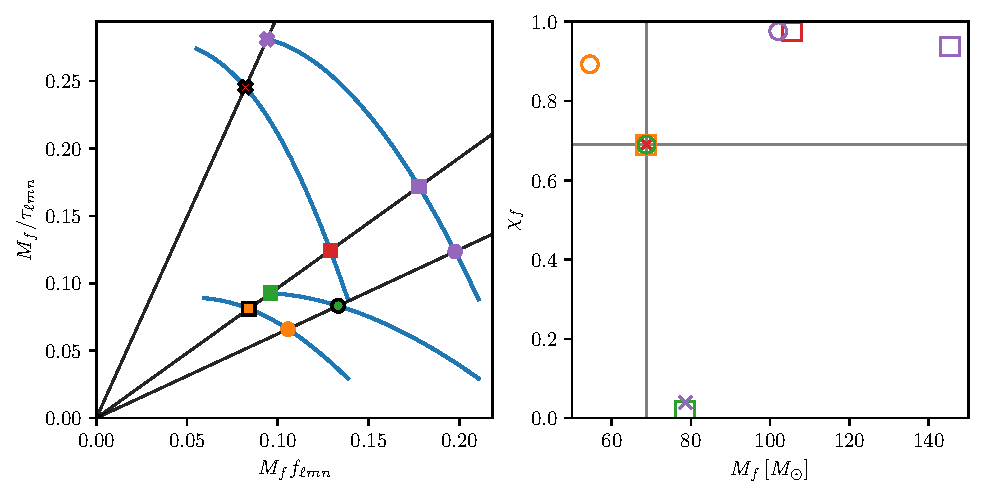
\includegraphics[width=\columnwidth]{Figures/Introduction/bh_spectroscopy.pdf}
    \caption[Black-hole spectroscopy illustration]{
    BH spectroscopy (inspired by a similar figure in Ref.~\cite{Dreyer:2003bv}): a frequency -- damping-time measurement corresponds to a straight line in the left panel. Three such measurements are shown, and their intersections with the Kerr spectrum are indicated. Each measurement is associated with a particular marker shape, and each Kerr branch is associated with a particular marker colour. Each intersection can be converted to a remnant BH mass and spin, shown on the right panel. Only one mass and spin is consistent with all three measurements; these are the true BH properties.
    }
    \label{ch1:fig:bh_spectroscopy}
\end{figure}

Fig.~\ref{ch1:fig:bh_spectroscopy} (inspired by a similar figure in Ref.~\cite{Dreyer:2003bv}) demonstrates the idea behind BH spectroscopy.
On the left panel we show four branches of the Kerr spectrum; the $(2,2,0)$, $(2,2,1)$, $(3,3,0)$ and $(3,3,1)$ modes.
The $(2,2,1)$ and $(3,3,0)$ modes are promising targets for a QNM measurement beyond the fundamental mode, and currently they are the only modes for which there is possible evidence in GW observations~\cite{Isi:2019aib, Capano:2021etf} (these claims are, however, disputed; see Chapter~\ref{Chapter4} for further discussion).
In BH spectroscopy, we imagine directly measuring a frequency and damping time in the GW data; say, $f_*$ and $\tau_*$.
In the $M_f f_{\ell m n}$ -- $M_f/\tau_{\ell m n}$ space, this measurement corresponds to a straight line intersecting with the origin; this simply comes from the fact that our scale is not fixed, since we express everything in terms of $M_f$. 
Fixing the value of $M_f$ would collapse the line to a single point, $(f_*,\tau_*)$.
The gradient of the line is given by
\begin{equation}
    \frac{1}{f_* \tau_*} = \frac{\pi}{Q_*},
\end{equation}
where $Q_* = \pi f_* \tau_*$ is the quality factor of the measured mode.
We show three such measurements, and mark where they intersect the Kerr spectrum.
Each intersection corresponds to a particular remnant BH mass, $M_f$, and spin, $\chi_f$. 
The distance of the intersection along the Kerr branch gives the spin.
The mass is found by, for example, dividing the value of $M_f f_{\ell m n}$ at the intersection by the measured frequency $f_*$.
Since each measurement line will generically intersect with multiple Kerr branches, they return multiple $(M_f, \chi_f)$ values. 
However, assuming the BH is indeed described by the Kerr metric, then there will be a single $(M_f,\chi_f)$ combination consistent with all the measurements (indicated by the horizontal and vertical lines in the right panel).
If no such combination exists, then what is observed is either not an isolated BH, or it is not described by the Kerr metric in GR. 

The above describes the key idea behind BH spectroscopy, but in practice the test is performed slightly differently.
Firstly, in reality it may not be practical to measure multiple QNM frequencies directly due to parameter degeneracies that come with summing functionally equivalent QNMs.
And secondly, it can be tricky to turn multiple frequency--damping-time measurements into a quantitative statement regarding compatibility with the GR Kerr spectrum.
With the expectation that what we measure will not be greatly different from the GR Kerr prediction, we can target the loudest QNMs in the data and parameterise all the QNM frequencies with a single mass and spin (according to the Kerr spectrum).
That is,
\begin{equation}
    \omega_{\ell m n} = \omega_{\ell m n}(M_f, \chi_f).
\end{equation}
This reduces the dimensions of the problem, and also directly measures the physically relevant properties of the remnant BH.
To measure any disagreement with the Kerr prediction, we allow a subset of the QNMs in our model to deviate from Kerr in the following way:
\begin{equation}
    f = f_{\ell m n}(M_f, \chi_f) e^{\delta f_{\ell m n}} \qquad \tau = \tau_{\ell m n}(M_f, \chi_f) e^{\delta \tau_{\ell m n}}.
\end{equation}
We emphasise that not all the modes in the model should be allowed to vary, since then the analysis becomes equivalent to a direct search of frequencies and damping times.
The new parameters, $\delta f_{\ell m n}$ and $\delta \tau_{\ell m n}$, will have measurements consistent with zero if the data is well described by Kerr.
Additionally, the uncertainty on the measurements of the $\delta$ parameters give us a natural test confidence. 
This method of testing the no-hair theorem is described further in Ref.~\cite{Isi:2021iql}, and is employed in Section~\ref{subsec:verify} for our analysis of GW150914.

% Chapter 2

\chapter{Modelling the Ringdown from Precessing Black-hole Binaries}

\label{Chapter2}

\section{Introduction}

A prerequisite for any ringdown analysis is a suitable choice for the \emph{start time}, $t_0$, of the ringdown. 
Starting too early risks a GW signal contaminated with nonlinearities that cannot be described by a model based solely on QNMs and obtaining biased measurements as a result. 
On the other hand, starting too late leaves a short signal that is already decaying and without enough signal-to-noise to make useful measurements. 
The difficulties of defining a suitable start time and some surprising data analysis consequences of this were discussed in \cite{Thrane:2017lqn}. 
Previous studies on numerical relativity (NR) waveforms have tended to use just a single \cite{Flanagan:1997sx} or relatively small number ($\leq 4$) \cite{Kamaretsos:2011um, London:2014cma, Carullo:2018sfu, Bhagwat:2017tkm} of QNMs, and have used a wide range of start times. 
Typically, the start time is referred to the maxima of some time-dependent quantity (e.g.\ the 22 mode of the strain, the modulus of the Weyl scalar, or the total GW luminosity; these quantities peak at times that typically differ by a few tens of $M$) and typical choices were ${10-20M}$ after the peak (although, see \cite{Berti:2007fi} where a range of different start times are explored). 
Several studies caution against starting too early \cite{JimenezForteza:2020cve, Bhagwat:2019dtm}.

More recently, \cite{Giesler:2019uxc} (see also \cite{Ota:2019bzl}) looked to allow the ringdown to start significantly earlier by including multiple overtones. 
In particular, \cite{Giesler:2019uxc} found that by including up to seven overtones the ringdown analysis can be started as early as the peak in the 22 mode of the strain. 
This might be considered a surprising result; the signal peak is expected to occur when the remnant BH (to the extent that it yet even makes sense to consider it as such) is most highly distorted and linear perturbation theory is not expected to be valid. 
The failure of this intuition was investigated in \cite{Okounkova:2020vwu} which suggests much of the nonlinearity is trapped behind a forming common apparent horizon and never makes it out to future null infinity in the form of GWs. 
Even more surprising, in \cite{Dhani:2020nik} this approach was extended by the inclusion of mirror modes along with overtones (thereby doubling the number of QNMs) and it was found that it was possible to start the ringdown analysis even earlier (up to ${10M}$ \emph{before} the peak). 
Clearly it is not surprising that a model with so many free parameters is able to fit the GW signal well; the important point is that it is able to do so without obtaining biased values for the final mass and spin. 
A ringdown model with overtones was successfully applied to GW150914 in \cite{Isi:2019aib} to extract the fundamental QNM and the first overtone from the noisy data, and more recently to events in GWTC-2 \cite{LIGOScientific:2020tif}. 

To the best of our knowledge, previous studies modelling the ringdown from NR simulations with QNMs have only considered aligned-spin BBH systems. 
We note that some work on precessing systems has been done in the extreme mass ratio limit, see \cite{Hughes:2019zmt,Lim:2019xrb}. 
It is well known that misalignment between the orbital angular momentum and the spins of the component BHs cause the orbit to precess during the inspiral phase of the evolution leading to qualitatively different GW signals at early times (e.g.\ see \cite{Apostolatos:1994mx}). 
It is less clear what effect, if any, misaligned component spins would have on the late time ringdown signal which is generally associated with the remnant BH. 
The primary aim of this paper is to address this question by systematically extending the analyses of \cite{Giesler:2019uxc, Dhani:2020nik} to a large number of precessing BBH simulations from the SXS catalog \cite{Boyle:2019kee, Mroue:2013xna}. 
We find that for BBH systems with misaligned spins, and that exhibit precession during their inspiral phase, a model consisting only of overtones (with or without mirror modes) \emph{cannot} be reliably applied from the peak of the 22 strain. 
A more conservative ringdown start time corresponding to the peak of the energy flux improves reliability, but we still see significant variation in performance across different simulations. 
The introduction of a higher harmonic (QNMs with $\ell > 2$) to the overtone model helps to reduce this variation, hinting at the importance of mode mixing.

Previous studies have also focused on using full NR simulations to test ringdown models. 
In this paper we briefly investigate the use of surrogates, which provide an opportunity to test models over a continuous parameter space. 
We find caution should be taken, particularly for surrogates of precessing systems, due to errors in the surrogate waveforms.

In section \ref{aligned-spin-section} we reproduce some important results from \cite{Giesler:2019uxc, Dhani:2020nik}, which are later compared with those for precessing systems in section \ref{misaligned-spin-section}. 
With precessing systems, it is necessary to perform a rotation to account for the fact that the spin of the remnant BH will not be aligned with initial coordinate axes used to set up the simulation; the procedure for doing this is also discussed in section \ref{misaligned-spin-section}. 
In section \ref{surrogate-section} we comment on the use of NR surrogates to test ringdown models. 
Finally, concluding remarks are presented in section \ref{sec:discussion}. 
Throughout, we use natural units in which $G=c=1$.

\section{Aligned-spin Systems}\label{aligned-spin-section}

As well as reproducing important results for spin-aligned systems \cite{Giesler:2019uxc, Dhani:2020nik}, this section introduces QNM modelling and describes our numerical fitting procedure. 

The GW signal far from a source of mass $M$ can be expanded in spin-weight $s=-2$ spherical harmonics as
\begin{equation}\label{YlmExpansion}
    h(t,r,\theta,\phi) = \frac{M}{r} \sum_{\ell = 2}^{\infty} \sum_{m = -\ell}^{\ell} h_{\ell m}(t) ~ {}_{-2}Y_{\ell m}(\theta, \phi).
\end{equation}
The $h_{\ell m}(t)$ coefficients are referred to as the spherical harmonic modes of the GW signal.
The ${\ell=|m|=2}$ modes are typically largest, while the remaining ``higher modes'' are generally subdominant.
The output of an NR simulation usually includes the first few modes (e.g.\ $\ell \leq 8$) with the asymptotic radial dependence scaled out.
The spherical harmonic modes are defined with respect to a particular frame at infinity.
This frame is chosen to be one in which the centre-of-mass of the system is at rest at some initial time; but this still leaves freedom to perform an overall rotation.
By convention, the \emph{NR frame} $(\theta,\phi)$ is uniquely fixed by requiring that initially the two component BHs are located on the $x$-axis and the orbital angular momentum, $\vb*{L}$, points along the $z$-axis.

At late times ($t \geq t_0$, where $t_0$ is to be determined) the signal is modelled as a sum of QNMs.
We note that as QNMs are not \emph{complete}, in the sense of being derivable from a self-adjoint operator, this model is necessarily an approximation.
The most general QNM ringdown model is a sum over $(\ell,m,n)$ including both the regular ($\omega_{\ell m n}$) and the mirror ($\omega'_{\ell m n}$) mode frequencies (see, e.g.\ \cite{Berti:2005ys}),
\begin{align}\label{general_ringdown}
    h(t,r,\theta',\phi') = \frac{M_f}{r} \sum_{\ell=2}^{\infty}\sum_{m=-\ell}^{\ell}\sum_{n=0}^{\infty} \big[ &C_{\ell m n} e^{-i \omega_{\ell m n}(t-t_0)} ~ {}_{-2}S_{\ell m n}(\theta',\phi') \\
    + &C'_{\ell m n} e^{-i \omega'_{\ell m n}(t-t_0)} ~ {}_{-2}S'_{\ell m n}(\theta',\phi') \big],
\end{align}
for $t\geq t_0$.
Here, ${}_{-2}S_{\ell m n}(\theta',\phi')$ are the spheroidal harmonics of spin weight $-2$, which are the most natural angular basis for the radiation produced by a perturbed Kerr BH. 
The prime on the second spheroidal harmonic is due to the different QNM frequency associated with the mirror modes.
They are related to the regular mode spheroidal harmonics by ${}_{-2}S'_{\ell m n}(\theta',\phi') = {}_{-2}S^*_{\ell (-m) n}(\pi-\theta',\phi')$ \cite{Dhani:2020nik}.
This model is constructed in the \emph{ringdown frame} $(\theta', \phi')$ in which the remnant BH is at rest with its spin vector pointing along the positive $z$-direction (such a frame is unique up to an unimportant $\phi'$ rotation about the $z$-axis).
For aligned-spin BBH systems, which do not precess during the inspiral, the ringdown and NR frames remain aligned with each other (at least up to an overall sign; some systems with strongly negative component spins can exhibit ``spin flip'' where the final spin points in the negative $z$-direction).
For misaligned-spin systems the remnant spin can point in essentially any direction and the NR and ringdown frames are misaligned.
The ringdown frame will also be moving with respect to the NR frame as a result of the recoil, or \emph{kick}, from the anisotropic emission of GWs near merger. The kick direction serves to single out a preferred $\phi'$ direction in the ringdown frame.
The effects of the kick are neglected here; it is assumed that the NR and ringdown frames are related by a rotation (see section \ref{misaligned-spin-section}).

Following Giesler \emph{et al.} \cite{Giesler:2019uxc}, the spherical harmonic modes of the ringdown signal can be modelled by writing each as a sum of $N$ overtones:
\begin{equation}\label{GieslerRD}
    h_{\ell m}^N(t) = \sum_{n=0}^N C_{\ell m n} e^{-i\omega_{\ell m n}(t-t_0)}, \quad \textrm{for} \quad t \geq t_0.
\end{equation}
This \emph{overtone} model is a restriction of the sum in Eq.~\ref{general_ringdown}, where overlaps between different harmonic $\ell$ indices (mode mixing) \cite{Berti:2014fga} as well as mirror modes are neglected. 
As in \cite{Giesler:2019uxc}, we model each spherical harmonic mode individually as a sum of QNMs. An alternative approach would be to model several spherical harmonic modes simultaneously with a shared set of QNM amplitudes which might give improved fits, especially when mode mixing is significant (see, e.g.\ \cite{Cook:2020otn}).
In \cite{Giesler:2019uxc}, the efficacy of this model for $l=m=2$ was demonstrated by performing least squares fits to the $h_{22}(t)$ mode for a selection of aligned-spin SXS simulations. The authors note that this was also verified for other values of $(\ell,m)$.

The overtone model in Eq.~\ref{GieslerRD} contains $2(N+1)$ free parameters in the complex amplitudes, $C_{\ell m n}$, plus the two parameters $M_f,\; \chi_f$ that determine the $\omega_{\ell m n}$ frequencies.
All of these parameters depend on the properties of the progenitor binary, but we do not study these dependencies here.
We now briefly describe the numerical procedure used to search over these parameters and obtain a least-squares fit with the NR strain data $\vb{d}=h_{\ell m}(t)$.
Writing the difference between $\vb{d}$ and the overtone model in Eq.~\ref{GieslerRD} in its discretely sampled form (at times $t_0,\, t_1,\, \dots,\, t_{K-1}$) gives a linear matrix equation (we temporarily drop $\ell$ and $m$ indices for clarity),
\begin{equation}\label{eq:linalg_fit}
\renewcommand*{\arraystretch}{1.5}
    ||\vb{d}-h^{N}_{\ell m}(t)|| = \norm{\mqty(d(t_0) \\ d(t_1) \\ \vdots \\ d(t_{K-1})) - 
    \mqty(e^{-i\omega_0(t_0-t_0)} & e^{-i\omega_1(t_0-t_0)} & \cdots & e^{-i\omega_N(t_0-t_0)} \\ 
          e^{-i\omega_0(t_1-t_0)} & e^{-i\omega_1(t_1-t_0)} & \cdots & e^{-i\omega_N(t_1-t_0)} \\ 
          \vdots & \vdots & \ddots & \vdots \\ 
          e^{-i\omega_0(t_{K-1}-t_0)} & e^{-i\omega_1(t_{K-1}-t_0)} & \cdots & e^{-i\omega_N(t_{K-1}-t_0)}) 
    \mqty(C_0 \\ C_1 \\ \vdots \\ C_N)}.
\end{equation}

Our fitting algorithm minimises the sum-of-the-squares of the fit residuals, which is the quantity in Eq.~\ref{eq:linalg_fit}. 
We find it convenient to treat the remnant property parameters $M_f$ and $\chi_f$ differently from the excitation amplitudes $C_n$. 
First, a discrete 2-dimensional numerical grid of values for 
$M_f$ and $\chi_f$ is constructed.
At each point on this grid, we consider varying only the complex amplitudes $C_n$. 
Eq.~\ref{eq:linalg_fit} turns this minimisation problem into a linear algebra problem that can be efficiently solved with, for example, \texttt{numpy.linalg.lstsq} \cite{Harris:2020xlr}.
Finally, the point of the grid with the lowest overall value for the sum-of-the-squares of the fit residuals is chosen.

\begin{figure}[t]
    \centering
    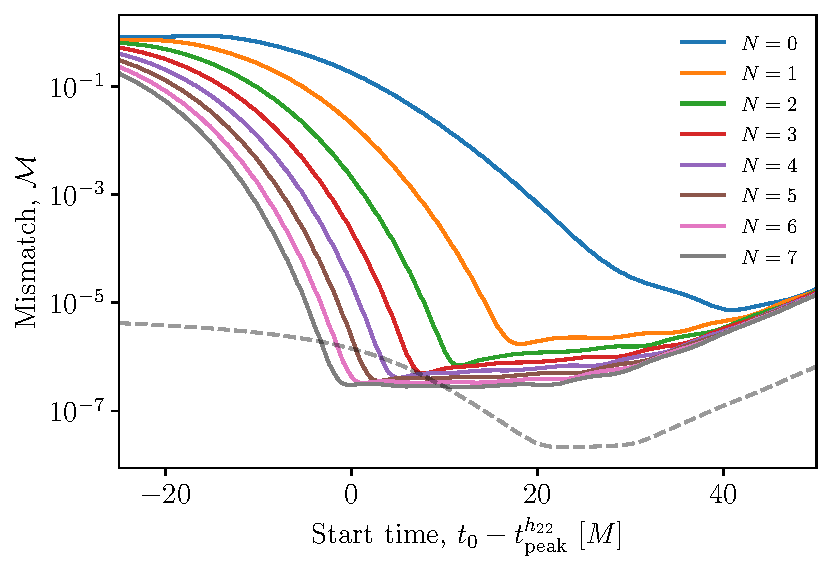
\includegraphics[width=0.8\columnwidth]{ModellingTheRingdownFromPrecessingBlackHoleBinaries/305_mismatch_vs_t0_with_error.pdf}
    \caption[Mismatch as a function of ringdown start time for an overtone model fitted to SXS:BBH:0305]{ 
    Mismatch for the overtone model (Eq.~\ref{GieslerRD}) when fitting to the NR simulation SXS:BBH:0305 as a function of ringdown start time $t_0$. When using only a single QNM (the fundamental $(\ell,m,n)=(2,2,0)$) the start time that gives the lowest mismatch with the NR data is well after the merger (the rising mismatch at late times is a numerical artefact). However, reproducing the results from \cite{Giesler:2019uxc}, we find that by including $N=7$ overtones the GW signal can be modelled using QNMs starting from as early as the peak strain. The dashed grey curve shows the estimate of the error in the underlying NR simulation and is described in appendix \ref{NR_error_appendix}.}
	\label{305_mismatch_vs_t0}
\end{figure}

\begin{figure}[t]
    \centering
    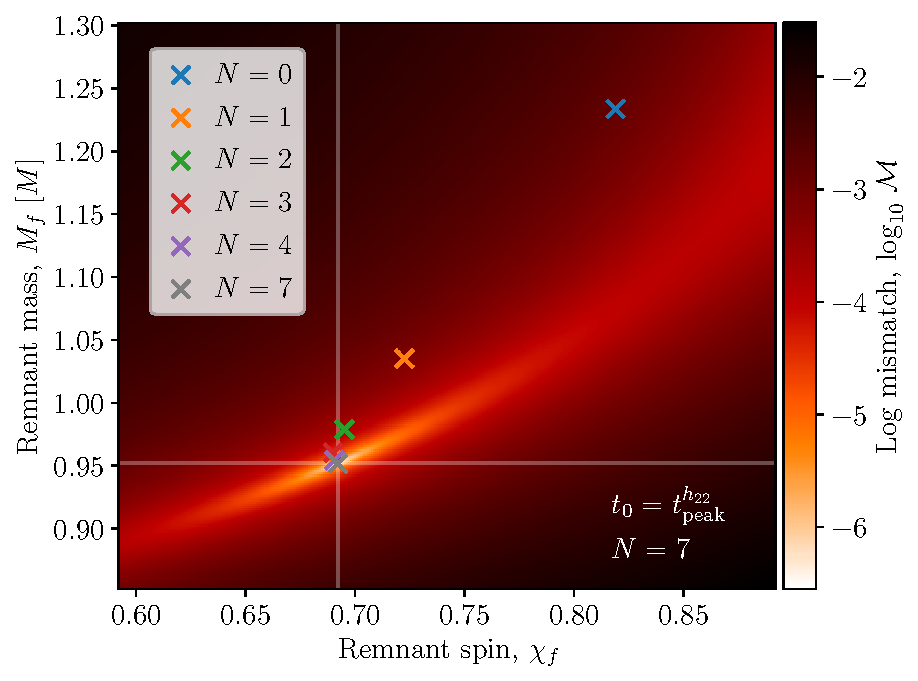
\includegraphics[width=0.8\columnwidth]{ModellingTheRingdownFromPrecessingBlackHoleBinaries/305_epsilon_grid.pdf}
    \caption[Recovery of the SXS:BBH:0305 remnant properties using an overtone model starting from the peak of the $h_{22}$ strain]{ 
    Recovery of the remnant properties for the overtone model (Eq.~\ref{GieslerRD}) when fitting to the NR simulation SXS:BBH:0305 starting from the peak in the $h_{22}$ strain.
    The heat map shows the mismatch for the fit with $N=7$ overtones, which shows a pronounced minimum close ($\epsilon=3.4\times 10^{-4}$) to the true remnant parameters (indicated by the horizontal and vertical lines).
    The sequence of crosses shows the locations of the minima for fits performed with the overtone model using different values of $N$, all using the same start time (the cross colours correspond to the colours used in Fig.~\ref{305_mismatch_vs_t0}; crosses for $N=5$ and 6 are omitted to avoid crowding the plot, but they converge towards the true remnant parameters). 
    If we choose a different ringdown start time for each $N$ corresponding to the mismatch minima in Fig.~\ref{305_mismatch_vs_t0}, we do see a reduction in $\epsilon$ for the lower $N$ models, however the $N=7$ model with $t_0=t_{\rm peak}^{h_{22}}$ remains the best performing model.
    } 
    \label{305_epsilon_grid}
\end{figure}

Once the least-squares fit to the data has been obtained, the quality, or \emph{goodness-of-fit}, is quantified via the mismatch and the error on the remnant parameters.
The \emph{mismatch} between signals $h_1$ and $h_2$ is defined as
\begin{equation}\label{mismatch}
    \mathcal{M} = 1 - \frac{\abs{ \braket{h_1}{h_2} }}{\sqrt{\braket{h_1}\braket{h_2}}},
\end{equation}
where we use the following complex inner product \cite{Nollert:1998ys}
\begin{equation} \label{eq:inner_prod}
    \braket{h_1}{h_2} = \int_{t_0}^T h_1(t) h^*_2(t) ~ \dd t.
\end{equation}
We integrate from the ringdown start time, $t_0$, to an upper limit $T$ chosen such that the whole ringdown is captured (we use $T = t_0 + 100M$).
When fitting models with very small mismatches, the finite accuracy of the NR simulations must be considered; this is discussed in appendix \ref{NR_error_appendix}.
As noted in \cite{Giesler:2019uxc}, a small mismatch is not sufficient by itself to justify the model.
The overtone model contains more parameters as $N$ is increased, and it is necessary to check for over-fitting.
To address this, we check to see if the remnant BH properties are correctly recovered by the model. 
The combined error on the remnant mass and spin is quantified by \cite{Giesler:2019uxc}
\begin{equation} \label{eq:epsilon}
    \epsilon = \sqrt{ \qty( \frac{\delta M_f}{M} )^2 + \qty( \delta\chi_f )^2 },
\end{equation}
where $\delta M_f = M_{\mathrm{best fit}} - M_f$, and $\delta \chi_f = \chi_{\mathrm{best fit}} - \chi_f$. 
The best fit values are those which minimise the mismatch, while the true values are taken from the metadata for the SXS simulation.
A ringdown model can be said to perform well if it yields small values for \emph{both} $\mathcal{M}$ and $\epsilon$.

\begin{figure*}[t]
    \centering
    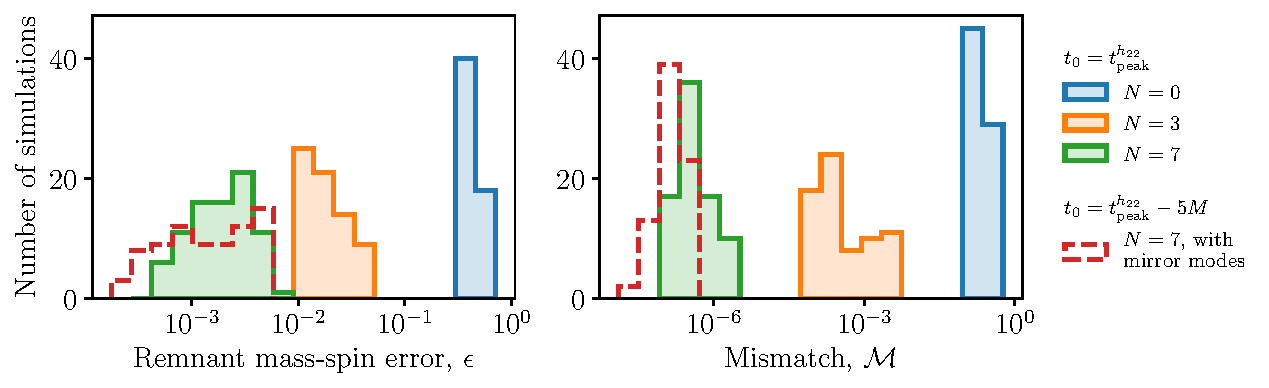
\includegraphics[width=\columnwidth]{ModellingTheRingdownFromPrecessingBlackHoleBinaries/aligned_spin_epsilon_M_hist.pdf}
    \caption[Remnant error and mismatches for fits to aligned-spin SXS simulations using an overtone model]{Left: histograms of the mass-spin remnant error $\epsilon$ from an overtone model fit to 85 aligned-spin SXS simulations for several different overtone numbers $N$. 
    Right: histograms of the mismatch from a fit with the true remnant mass and spin parameters, with the same overtone models and SXS simulations as in the left histogram.
    The solid histograms show results from fits performed starting at the peak of the $h_{22}$ mode with $N$ overtones of the fundamental $\ell = m = 2$ mode.
    The red dashed line shows results from a $N=7$ model that also includes mirror modes (see section \ref{subsec:mirror_modes}) and was fitted with a ringdown starting $5M$ before the peak in the strain.}
    \label{aligned_spin_epsilon_hist}
\end{figure*}

Following \cite{Giesler:2019uxc}, we now apply these ideas to the simulation SXS:BBH:0305 \cite{Lovelace:2016uwp, sxs_catalog}.
This simulation has source parameters consistent with GW150914 and was originally chosen to demonstrate the success of the overtone model. 
Fig.~\ref{305_mismatch_vs_t0} shows the mismatch values obtained with the overtone model when using the true values of $M_f$ and $\chi_f$.
With $N=7$ (that is, eight QNMs = the fundamental + seven overtones) the $h_{22}(t)$ mode can be fitted all the way back to the time of its peak amplitude, $t_{\mathrm{peak}}^{h_{22}}$, while still achieving the smallest possible mismatch.
Using a smaller number of overtones requires a later choice for the start time to achieve the smallest possible mismatch.
In addition to giving a small ($\sim 10^{-6}$) mismatch, the $N=7$ overtone model, with $t_0 = t_{\mathrm{peak}}^{h_{22}}$, also achieves this minimum mismatch with the correct values for the remnant properties; this is shown by the heat map in Fig.~\ref{305_epsilon_grid} where the values of $M_f$ and $\chi_f$ are now allowed to vary. 
We find, for the $N=7$ model, a remnant error $\epsilon = 3.4 \cross 10^{-4}$. 
Importantly, this is larger than the NR error on the remnant properties (which is estimated to be $\epsilon_{\mathrm{NR}} = 2.1 \cross 10^{-5}$, see appendix \ref{NR_error_appendix} for details). This confirms that this is really the true scale of the bias in the inferred remnant parameters when using the overtone model, and not just the numerical noise floor in the NR simulation.
Again, using a smaller number of overtones and starting the ringdown as early as $t_{\mathrm{peak}}^{h_{22}}$ gives inferior results with the minimum in the mismatch being biased away from the true parameters.
The results in Figs.~\ref{305_mismatch_vs_t0} and \ref{305_epsilon_grid} show that the overtone model performs well for SXS:BBH:0305 (i.e.\ yields small $\mathcal{M}$ and $\epsilon$) even when starting the ringdown as early as the peak in the strain.

In order to see how robust the conclusions drawn from SXS:BBH:0305 are in general, the calculations of $\epsilon$ and $\mathcal{M}$ were repeated for a wider selection of SXS simulations. Following \cite{Giesler:2019uxc}, we consider only aligned-spin simulations with initial spin magnitudes $|\vb*{\chi}_{1,2}| = \chi_{1,2} < 0.8$, and mass ratios $q < 8$. We also require that the $z$-component of $\vb*{\chi}_f$ is greater than zero, which eliminates the ``spin flip'' systems. The simulations were chosen in the ID range SXS:BBH:1412 to SXS:BBH:1513, as these cover a range of initial spin magnitudes and mass ratios.
After applying these cuts, this left 85 spin-aligned SXS simulations in our test population.
For each simulation, fits were performed using the overtone model with $N=0$, 3, and 7 and with a start time of $t_0 = t_{\mathrm{peak}}^{h_{22}}$. 
The results are shown in Fig.~\ref{aligned_spin_epsilon_hist}. 
We see distributions similar to those in Fig.~3 of \cite{Giesler:2019uxc}. 
The inclusion of additional overtones systematically shifts the entirety of both the $\epsilon$ and $\mathcal{M}$ histograms to smaller values.
We note, as it will become important later, that the worst cases in these histograms improve, along with the median values.
This demonstrates that, when using the overtone model on systems with aligned spins, the ringdown reliably starts as early as the peak in the $h_{22}(t)$ mode of the strain. 


\subsection{Mirror Modes} \label{subsec:mirror_modes}

For a given $\ell$, $m$ and $n$, the equations governing QNM frequencies allow two solutions: one, $\omega_{\ell m n} = 2\pi f_{\ell m n} - i/\tau_{\ell m n}$, with a positive real part; and another, $\omega'_{\ell m n} = 2\pi f'_{\ell m n} - i/ \tau'_{\ell m n}$, with negative real part \cite{Dhani:2020nik, Berti:2005ys}.
The frequencies of the mirror modes $\omega'_{\ell m n}$ are related to the regular modes $\omega_{\ell m n}$ by
\begin{equation}\label{mirrorsymmetry}
    f'_{\ell m n} = -f_{\ell -m n}, \quad \tau'_{\ell m n} = \tau_{\ell -m n} \nonumber
\end{equation}
\begin{equation} 
    \quad\Rightarrow\quad \omega'_{\ell mn} = - \omega_{\ell -mn}^*.
    \label{eq:sym_mirror_modes_conj}
\end{equation}

A new ringdown model which explicitly includes the mirror modes can be written as
\begin{align}
    h_{\ell m}^{N,\, {\rm mirror}}(t) = \sum_{n=0}^N \Big[& C_{\ell m n} e^{-i \omega_{\ell m n}(t-t_0)} \\ &+ C'_{\ell m n} e^{-i \omega'_{\ell m n}(t-t_0)} \Big]\quad \textrm{for} \quad t \geq t_0. \nonumber
\end{align}
This \emph{mirror mode} model is an extension of the overtone model in Eq.~\ref{GieslerRD};
if $C'_{\ell m n} = 0$ the mirror modes aren't excited and we recover the previous overtone model. 
This model has twice as many free parameters as the overtone model; $4(N+1)$ in the complex amplitudes, plus the two remnant parameters $M_f,\; \chi_f$.
The mirror mode model is still a restriction of the full sum in Eq.~\ref{general_ringdown} as overlaps between modes with different $\ell$ indices (i.e.\ mode mixing) are still not included.
Substituting for $\omega'_{\ell m n}$ using the conjugate symmetry property in Eqs.~\ref{eq:sym_mirror_modes_conj}, we can rewrite the mirror mode model in the form
\begin{align} \label{mirror_ringdown}
   h_{\ell m}^{N,\, {\rm mirror}}(t) = \sum_{n=0}^N \Big[& C_{\ell m n} e^{-i \omega_{\ell m n}(t-t_0)} \\ &+ C'_{\ell m n} e^{i \omega^*_{\ell -m n}(t-t_0)} \Big]\quad \textrm{for} \quad t \geq t_0. \nonumber
\end{align}
It is this form of the mirror mode model that was implemented.

As was shown in \cite{Dhani:2020nik}, the inclusion of mirror modes can improve the ringdown modelling of aligned-spin systems. In particular, the ringdown can be considered to start even earlier in the waveform, whilst still recovering the correct remnant properties. We confirm this here by repeating the above analysis for the same set of spin-aligned SXS simulation, but now using the mirror mode model in Eq.~\ref{mirror_ringdown} with $N=7$ and an earlier choice for the ringdown start time, $t_0 = t_{\mathrm{peak}}^{h_{22}} - 5M$.
Although \cite{Dhani:2020nik} demonstrated the mirror mode model starting $10M$ before the peak in the $h_{22}$ strain, we adopt a more conservative choice of $5M$.
The results are shown in Fig.~\ref{aligned_spin_epsilon_hist} plotted using a dashed line. 
The addition of mirror modes gives a small improvement in the mismatch, but this is to be expected with the increased number of parameters.
However, the $\epsilon$ histogram shows that the overall performance of the mirror mode model is comparable to that of the $N=7$ overtone model, despite the use of an earlier start time.


\section{Misaligned-spin Systems}\label{misaligned-spin-section}

The analyses in section \ref{aligned-spin-section}, and in the previous studies \cite{Flanagan:1997sx, Berti:2007fi, Kamaretsos:2011um, London:2014cma, Carullo:2018sfu, Bhagwat:2017tkm, Giesler:2019uxc, Ota:2019bzl, Dhani:2020nik}, was limited to BBH systems with component spins that are aligned with the orbital angular momentum, $\vb*{L}$.
This is a potentially serious limitation as misaligned spins are expected to be a generic feature of astrophysical BBHs.
Misaligned spins generally lead to precession of the orbital plane during the inspiral phase of the evolution and a richer phenomenology in the GW signals \cite{Apostolatos:1994mx}.
Several of the GW detections already show signs of precession, both individually \cite{LIGOScientific:2020ibl, Gerosa:2020aiw} and when considered as a population \cite{LIGOScientific:2020kqk}.
Most notably for our present purposes, the very high-mass system GW190521 \cite{LIGOScientific:2020iuh, LIGOScientific:2020ufj} might show some signs of precession while also having a high fraction of the observable signal-to-noise ratio in the ringdown. 
In this section we investigate the effect of precession on the modelling of the ringdown by repeating analyses like those in section \ref{aligned-spin-section}, but now on precessing NR simulations.

The general ringdown signal in Eq.~\ref{general_ringdown} is written in the ringdown frame $(\theta', \phi')$ which is aligned with the remnant spin vector (i.e.\ $\vb*{\chi}_f$ points along the positive $z$-direction in this frame). For BBH systems with misaligned spins that undergo precession, the ringdown frame differs from the frame typically used in NR simulations $(\theta, \phi)$ which is aligned with $\vb*{L}$ at some arbitrary start time in the inspiral.
These two frames are related by a rotation, $\mathbf{R}$.

The direction from which a GW source is viewed affects the observed signal 
(e.g.\ you see circularly/linearly polarised GWs with a larger/smaller amplitude when viewing parallel/perpendicular to $\vb*{L}$).
These differences in the GW signals also manifest themselves at the level of individual modes as amplitude modulations. The frame in which the expansion is performed affects the values of the spherical harmonic modes. 
The GW signal, originally given in the NR frame in Eq.~\ref{YlmExpansion}, can be re-expanded in the ringdown frame as follows:
\begin{equation}\label{hprimedecomp}
    h'(t, r, \theta', \phi') = \frac{M}{r} \sum_{\ell = 2}^{\infty} \sum_{m = -\ell}^{\ell}  h'_{\ell m}(t) ~ {}_{-2}Y_{\ell m}(\theta', \phi').
\end{equation}
When analysing the ringdown, it is most natural to use the spherical harmonic modes in the ringdown frame, $h'_{\ell m}(t)$, as these are adapted to the remnant BH. 
In particular, we will focus on modelling the $\ell = m = 2$ spherical harmonic mode in the ringdown frame, $h'_{22}(t)$.

\begin{figure}[b]
    \centering
    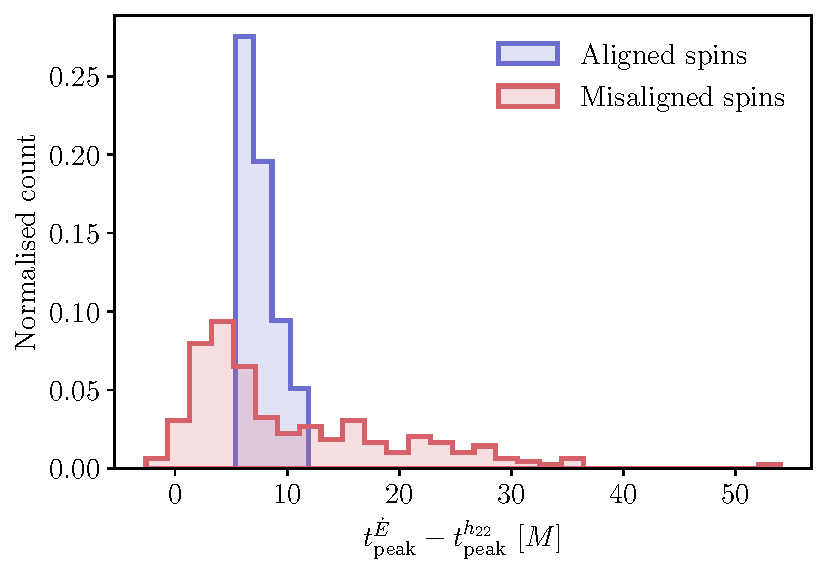
\includegraphics[width=0.8\columnwidth]{ModellingTheRingdownFromPrecessingBlackHoleBinaries/tEdot-t22_hist.pdf}
    \caption[Differences between the times of peak strain and peak GW energy flux]{  
    Histogram of the differences between the two possible start times considered in section \ref{misaligned-spin-section}: the peak of the (rotated) strain mode $h'_{22}$, and the peak of the GW energy flux.
    The normalised distribution of the differences between these times is shown both for the 85 spin-aligned systems used in section \ref{aligned-spin-section} and for the 252 precessing simulations considered in section \ref{misaligned-spin-section}. 
    The peak of the flux almost always occurs later than the peak of the strain, making this a more conservative choice for the ringdown start time. 
    We note that there is a much greater variation amongst the population with misaligned spins.
    }
	\label{tEdot-t22}
\end{figure}

For aligned-spin systems, the $h_{2\pm2}$ are usually the dominant modes in the sum in Eq.~\ref{YlmExpansion}. This is related to the fact that the GW signal amplitude is largest when viewed along the direction of the orbital angular momentum: $\vb*{L}$ or $-\vb*{L}$. For misaligned-spin systems undergoing precession, other modes become important. This in turn is related to the constantly changing direction of the orbital angular momentum, $\vb*{L}(t)$.
Changing into the non-inertial, \emph{coprecessing} frame in which $\vb*{L}$ always points along the $z$-direction has been found to account for most precessional effects and makes the precessing waveform remarkably similar to a non-precessing one.
This transformation into the coprecessing frame has been successfully used to help model the full inspiral-merger-ringdown waveforms for precessing systems \cite{Schmidt:2010it,Schmidt:2012rh} in the context of phenomenological \cite{Hannam:2013oca, Khan:2018fmp, Pratten:2020ceb}, effective-one-body \cite{Pan:2013rra, Ossokine:2020kjp} and NR surrogate \cite{Blackman:2017dfb, Blackman:2017pcm, Varma:2019csw} modelling.
There is an analogy with the approach taken here for the modelling of the ringdown. In order to simplify the task, we choose to work in a frame adapted to final spin angular momentum of the remnant, $\vb*{\chi}_f$.
Although, in our case, the rotation required to get into this frame is not time dependent and our chosen frame is therefore inertial.

\begin{figure}[t]
    \centering
    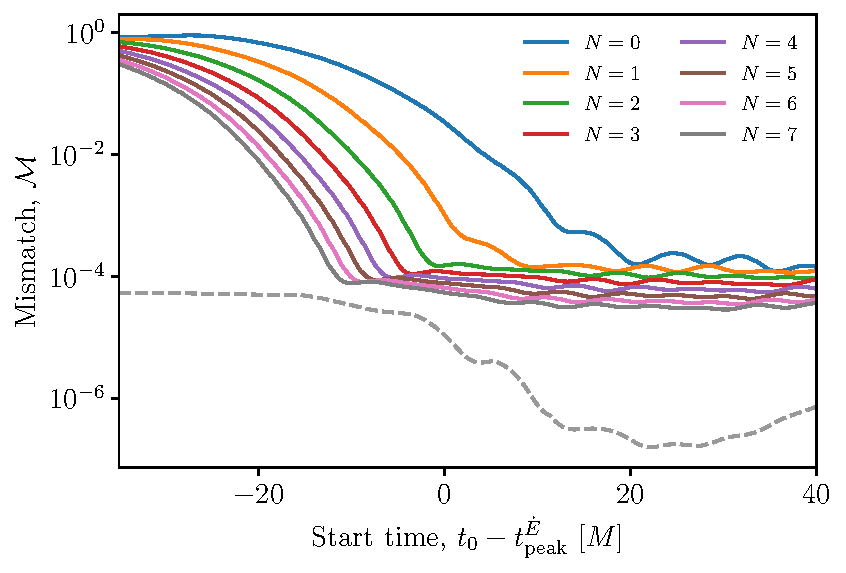
\includegraphics[width=0.8\columnwidth]{ModellingTheRingdownFromPrecessingBlackHoleBinaries/1856_mismatch_vs_t0_with_error_edit.pdf}
    \caption[Mismatch as a function of ringdown start time for an overtone model fitted to SXS:BBH:1856]{
    The mismatch for the overtone model (Eq.~\ref{GieslerRD}) when fitting to the NR simulation SXS:BBH:1856 as a function of ringdown start time $t_0$. When using $N=7$ overtones, the lowest mismatch is achieved starting slightly ($\sim 10M$) before the peak in the GW energy flux.
    However, the minimum mismatch is $\sim 100$ times larger than that obtained for the example spin-aligned system SXS:BBH:0305 in Fig.~\ref{305_mismatch_vs_t0}. The dashed grey curve shows the estimate of the error in the underlying NR simulation and is described in appendix \ref{NR_error_appendix}.
    }
    \label{1856_mismatch_vs_t0}
\end{figure}

The spin-weighted spherical harmonics, ${}_{-2}Y_{\ell m}$, transform in a particularly simple manner under rotations.
Rotations have the effect of mixing together modes with different $m$ indices, but preserving the same $\ell$. 
The mixing coefficients in these transformations are the Wigner $D$-matrices $D^{\ell}_{\mu m} (\mathbf{R})$.
The transformation properties of the ${}_{-2}Y_{\ell m}$ functions under rotations means that the rotated $h'_{\ell m}$ modes in the ringdown frame are related to the $h_{\ell m}$ modes in the NR frame (included in the NR output, and as used in section \ref{aligned-spin-section}) by the sum (see, for example \cite{Boyle:2013nka, Schmidt:2010it, OShaughnessy:2011pmr})
\begin{align}\label{Yrotation_wignerD}
    h'_{\ell m}(t) &= \sum_{\mu = -\ell}^{\ell} D^{\ell}_{\mu m} (\mathbf{R}) ~ h_{\ell \mu}(t).
\end{align}
The rotation $\mathbf{R}$ can be obtained from the direction of the remnant BH spin vector (which is provided as metadata for all SXS simulations). Specifically, $\mathbf{R}$ is any rotation that maps the $z$-axis onto the final spin vector.

\begin{figure}[t]
    \centering
    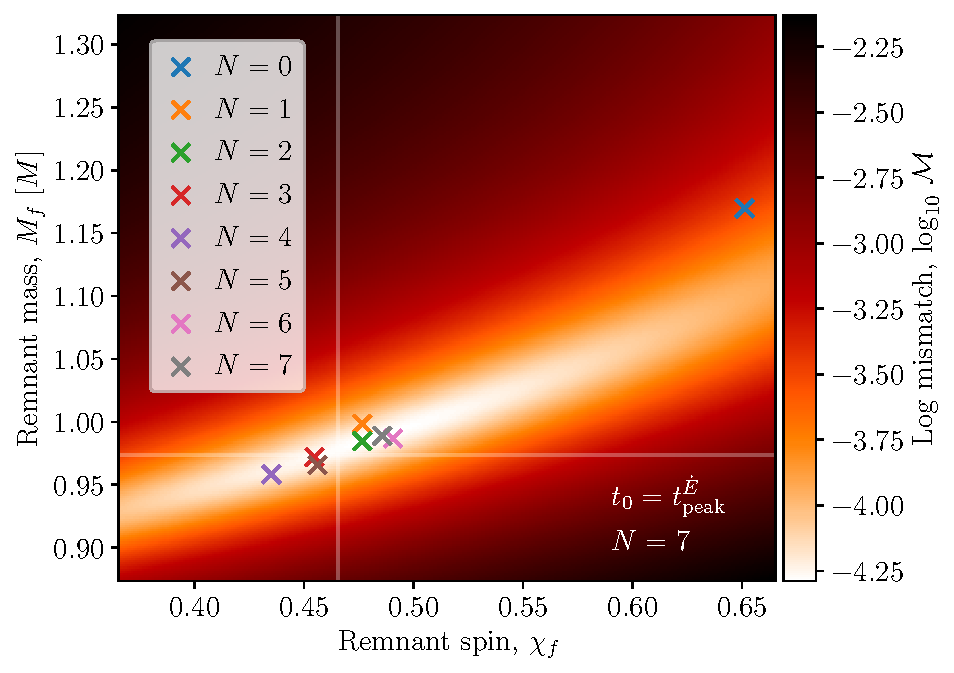
\includegraphics[width=0.8\columnwidth]{ModellingTheRingdownFromPrecessingBlackHoleBinaries/1856_epsilon_grid_alt.pdf}
    \caption[Recovery of the SXS:BBH:1856 remnant properties using an overtone model starting from the peak of the GW energy flux]{
    The recovery of the remnant properties for the overtone model (Eq.~\ref{GieslerRD}) when fitting to the NR simulation SXS:BBH:1856 starting from the peak in the flux.
    The heat map shows the mismatch for the fit with $N=7$, while the crosses show the locations of the minima in the mismatch for fits performed with different values of $N$.
    The mismatch shows a much broader and less deep minimum than that seen for the spin-aligned system SXS:BBH:0305 in Fig.~\ref{305_epsilon_grid}.
    The minimum in the mismatch is also biased away from the true remnant parameters with $\epsilon=0.025$ for the $N=7$ fit.
    The sequence of crosses for fits with different values of $N$ also do not show the same convergent trend towards the true remnant parameters that was observed for SXS:BBH:0305 in Fig.~\ref{305_epsilon_grid}.
	}
	\label{1856_epsilon_grid}
\end{figure}

We now apply the overtone model to the ringdown of an example precessing simulation SXS:BBH:1856 \cite{Varma:2019csw}. 
This simulation initially (at the reference time) has a mass ratio of $q=2.78$ and dimensionless spins $\vb*{\chi}_1=(0.18, -0.54, -0.45)$ and $\vb*{\chi}_2=(-0.12, -0.31, -0.031)$ on the heavier and lighter components respectively. This simulation was chosen because it exhibits strong precession effects visible as amplitude modulations in $h_{22}(t)$. The final spin vector is $\vb*{\chi}_f=(-0.03,-0.19,0.42)$ and the rotated mode $h'_{22}(t)$ was computed using Eq.~\ref{Yrotation_wignerD}.

\begin{figure*}[t]
    \centering
    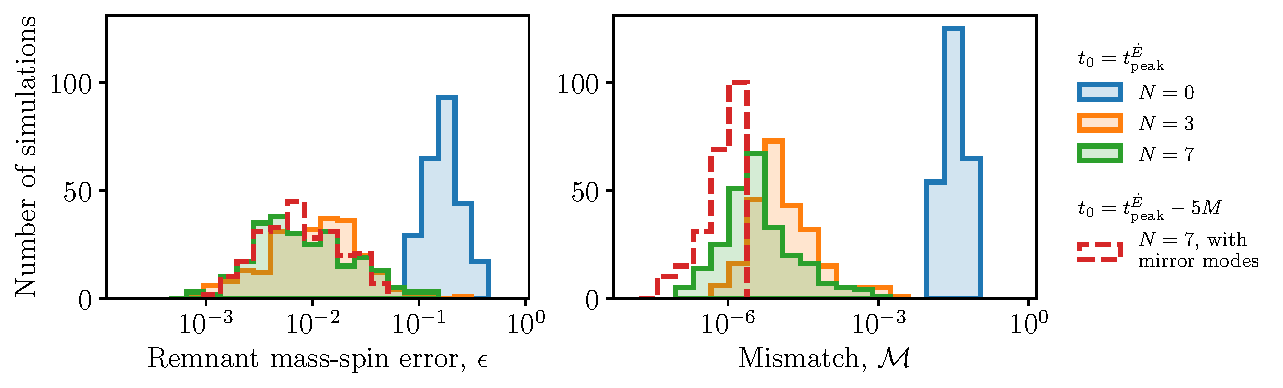
\includegraphics[width=\columnwidth]{ModellingTheRingdownFromPrecessingBlackHoleBinaries/misaligned_spin_epsilon_M_hist.pdf}
    \caption[Remnant error and mismatches for fits to misaligned-spin SXS simulations using an overtone model]{Left: histograms of the mass-spin remnant error $\epsilon$ from an overtone model fit to the rotated $h'_{22}$ modes of 252 misaligned-spin SXS simulations for several different overtone numbers $N$. 
    Right: histograms of the mismatch from a fit with the true remnant mass and spin parameters, with the same overtone models and SXS simulations as in the left histogram.
    The solid histograms show results from fits performed starting at the peak of the energy flux with $N$ overtones of the fundamental $\ell = m = 2$ mode.
    The red dashed line shows results from a $N=7$ model that also includes mirror modes and was fitted with a ringdown starting $5M$ before the peak in the energy flux.
    These histograms should be compared with those in Fig.~\ref{aligned_spin_epsilon_hist}; we note that the effect of precession is to (i) significantly broaden the histograms (i.e.\ the quality of the fit is much more varied) and (ii) to significantly degrade the quality of the fit for some systems.}
    \label{misaligned_spin_epsilon_hist}
\end{figure*}

The overtone model in Eq.~\ref{GieslerRD} was fitted to the rotated $\ell=m=2$ mode of the strain, $h'_{22}(t)$, in the same way as was done for the aligned-spin systems in section \ref{aligned-spin-section}.
There is some ambiguity in how to choose the ringdown start time $t_0$ in a way that gives as fair a comparison as possible with the non-precessing case.
We cannot use the peak of the $h_{22}(t)$ strain, as was done in section \ref{aligned-spin-section}, as this mode suffers from precession induced amplitude modulations. 
One option would be to use instead the peak of the rotated strain mode $h'_{22}(t)$.
However, we find that using the peak of the GW energy flux, $\dot{E}$, (which can be computed from the modes in either frame, see Eq.~3.8 in \cite{Ruiz:2007yx}) gives more consistent results between simulations. For example, some precessing configurations show a peak in the (rotated) strain relatively early in the signal, leading to poorer fits.
The use of the peak in the flux is also a conservative choice in the sense that $t_{\mathrm{peak}}^{\dot{E}} > t_{\mathrm{peak}}^{h_{22}}$ in almost all cases (see Fig.~\ref{tEdot-t22}).

Fig.~\ref{1856_mismatch_vs_t0} shows how the mismatch varies for SXS:BBH:1856 as a function of ringdown start time, for different values of $N$ in the overtone model Eq.~\ref{GieslerRD}.
With each additional overtone, the minimum mismatch is reached at an earlier time (the same behaviour as was seen in Fig.~\ref{305_mismatch_vs_t0}).
However, the values of the minimum mismatch are a factor of $\sim 100$ larger than those obtained in the aligned-spin case. 

The $N=7$ model achieves a minimum mismatch $\sim 10M$ before the time of peak GW energy flux. This is fairly typical behaviour among the misaligned-spin SXS simulations considered.
However, we note there is a much greater variety of possible behaviours for misaligned-spin systems than for the aligned-spin population. 
In order to emphasise this greater variation, in appendix \ref{appendix_a} we repeat the analysis in Figs.~\ref{1856_mismatch_vs_t0} and \ref{1856_epsilon_grid} for three more misaligned-spin simulations and highlight some of the observed differences. 
The greater variation amongst the misaligned-spin population has already been hinted at in Fig.~\ref{tEdot-t22}, where the spread of start times is greater than in the aligned-spin cases.

The heat map of Fig.~\ref{1856_epsilon_grid} shows the mismatch as a function of the remnant BH properties, for the $N=7$ model.
The coloured crosses indicate the mismatch minimum for different values of $N$. 
Comparing with Fig.~\ref{305_epsilon_grid}, we see the mismatch minimum is less pronounced than the aligned-spin case, which is probably contributing to the larger value of $\epsilon$ (for $N=7$ we find $\epsilon = 0.025$, which is much larger than the estimated numerical error $\epsilon_{\mathrm{NR}} = 8.6 \cross 10^{-5}$). 
In addition, the convergent behaviour with increasing $N$ is not present. For $N \geq 1$, all mismatch minima appear randomly distributed around the true remnant properties.
If we reproduce this figure with a earlier start time of $t_0 = t_{\mathrm{peak}}^{\dot{E}} - 10M$ (motivated by the time of minimum mismatch for $N=7$ in Fig.~\ref{1856_mismatch_vs_t0}), the heat map remains unchanged, and the value of $\epsilon$ recovered for $N=7$ is not significantly improved ($\epsilon = 0.013$). The earlier start time does cause the value of $\epsilon$ for $N \leq 3$ to increase significantly, which may be expected as we are now using a start time before those models reach a mismatch minimum. 

Following section \ref{aligned-spin-section}, we now extend this analysis to a wider selection of SXS simulations to investigate the robustness (or lack thereof) of this behaviour. We consider only misaligned-spin simulations, chosen such that the angle between the initial spins, $\chi_{\theta}$, satisfies $\pi/16 < \chi_{\theta} < 15\pi/16$. We again require initial spin magnitudes $\chi_{1,2} < 0.8$ and mass ratios $q<8$. The 252 simulations were chosen in the ID range SXS:BBH:1643 to SXS:BBH:1899, as these cover a range of mass ratios and initial spin configurations.

The results are shown in Fig.~\ref{misaligned_spin_epsilon_hist}. 
When compared to the $N=0$ model, the addition of three overtones reduces the remnant error and mismatch. 
However, the inclusion of additional overtones does not change the $\epsilon$ histogram, and produces only a minor reduction in the mismatch.
Comparing the $N=7$ histogram for $\epsilon$ to that found in Fig.~\ref{aligned_spin_epsilon_hist}, we see that, on average, $\epsilon$ increases by a factor of $\sim 10$ and, in the worst cases, by a factor of $\sim 20$ (however, the overtone model does still perform similarly well for a small fraction of simulations). 
The histograms for $\epsilon$ reflect the behaviour of Fig.~\ref{1856_epsilon_grid}, where models with $N \geq 1$ don't show systematic improvements. 
It would be interesting to investigate whether the binary parameters correlate with $\epsilon$, and if certain binary configurations are responsible for the largest remnant errors. We have performed preliminary studies which reveal no clear correlations of $\epsilon$ with either the amount of precession (quantified via $\chi_p$ \cite{Schmidt:2014iyl}) or the recoil velocity. We defer a more detailed study of this question to future work.

It was checked if using an earlier start time of $t_{\mathrm{peak}}^{\dot{E}} - 10M$ changed the recovered distribution on $\epsilon$. This choice was motivated by the location of the mismatch minimum typically seen for misaligned-spin simulations (e.g.\ see Fig.~\ref{1856_mismatch_vs_t0}). The results are shown in appendix \ref{misaligned_spin_fits_appendix}. It was found the $N=7$ model results did not significantly change. However, the $N=3$ and $N=0$ models performed worse.
Finally, we also note that all of the histograms are wider than those in Fig.~\ref{aligned_spin_epsilon_hist}. 
This may be due to mirror modes and/or higher harmonics having a more important role for precessing systems (see below). 

\begin{figure}[t]
    \centering
    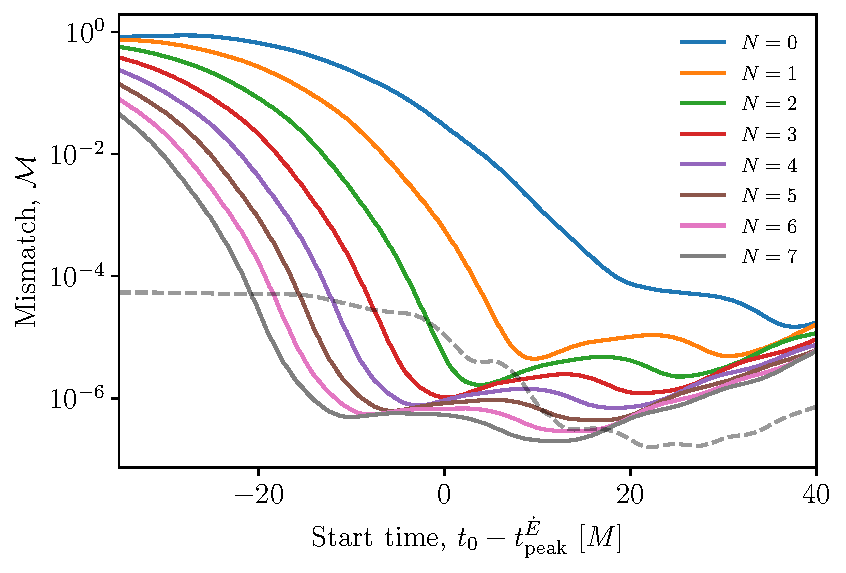
\includegraphics[width=0.8\columnwidth]{ModellingTheRingdownFromPrecessingBlackHoleBinaries/1856_mismatch_vs_t0_mirror_modes_with_error_edit.pdf}
    \caption[Mismatch as a function of ringdown start time for the mirror-mode model fitted to SXS:BBH:1856]{ 
    The mismatch for the mirror mode model (Eq.~\ref{mirror_ringdown}) fitted to the NR simulation SXS:BBH:1856 as a function of ringdown start time $t_0$. Comparing with Fig.~\ref{1856_mismatch_vs_t0}, the locations of the mismatch minima are roughly unchanged in time, but the inclusion of mirror modes reduces the mismatch to values similar to those in Fig.~\ref{305_mismatch_vs_t0}. The dashed grey curve shows the estimate of the error in the underlying NR simulation and is described in appendix \ref{NR_error_appendix}.
    }
	\label{1856_mirror_mode_mismatch_vs_t0}
\end{figure}


\subsection{Mirror Modes} \label{subsec:misaligned_mirror_modes}

We repeat the population analysis with the $N=7$ mirror mode model, again shifting the ringdown start time back by $5M$ to make a clear comparison to Fig.~\ref{aligned_spin_epsilon_hist}. 
The results are shown by the red dashed lines in Fig.~\ref{misaligned_spin_epsilon_hist}. The histogram for $\epsilon$ doesn't reach values as high as the overtone model (with worst-case values of $\epsilon \sim 0.04$ compared to the overtone model's $\sim 0.2$), but otherwise has a broadly similar distribution.
However, there is a significant improvement on the recovered mismatch values. This is expected because of the large number of parameters. And, as discussed, this alone isn't enough to say the model is successful.

Inspecting individual simulations, we see that the inclusion of mirror modes can make the mismatch minima in the mass-spin plane more pronounced (advantageous, as it reduces uncertainty on $\epsilon$). For example, Figs.~\ref{1856_mirror_mode_mismatch_vs_t0} and \ref{1856_mirror_mode_epsilon_grid} show how mirror mode fits perform for SXS:BBH:1856. 
We see significantly smaller mismatches, and a stronger mismatch peak around the true remnant properties. However, on average this does not translate to smaller values of $\epsilon$ for the $N=7$ model (as can be seen from the red dashed histogram in Fig.~\ref{misaligned_spin_epsilon_hist}). For SXS:BBH:1856, the $N=7$ model gives $\epsilon = 0.014$, which is not a significant improvement.

\begin{figure}[t]
    \centering
    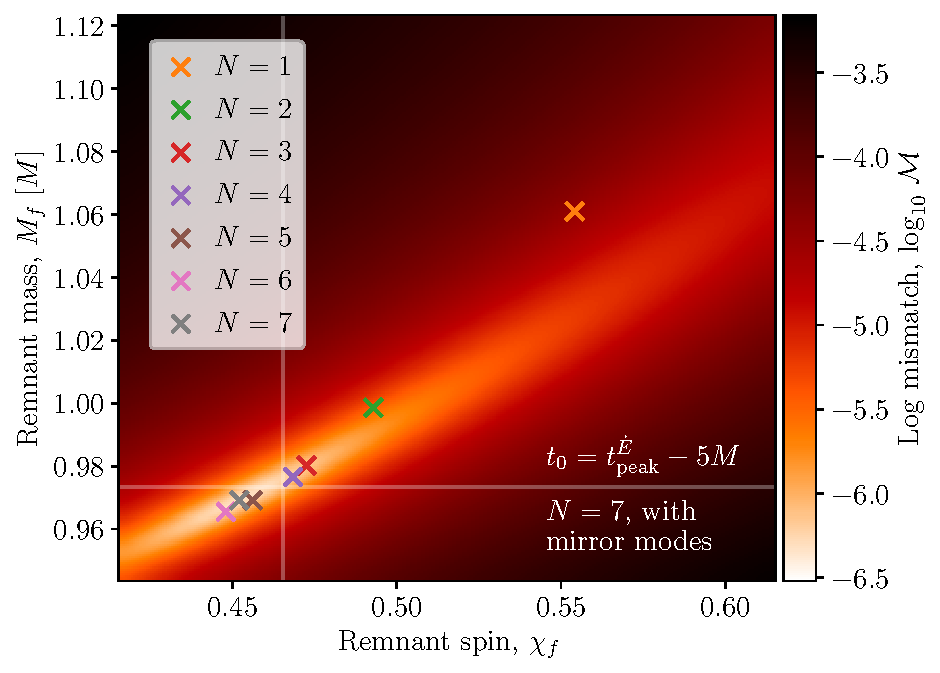
\includegraphics[width=0.8\columnwidth]{ModellingTheRingdownFromPrecessingBlackHoleBinaries/1856_epsilon_grid_mirror_modes_m5.pdf}
    \caption[Recovery of the SXS:BBH:1856 remnant properties using the mirror-mode model starting from $5M$ before the peak of the GW energy flux]{ 
    The recovery of the remnant properties for the mirror mode model (Eq.~\ref{mirror_ringdown}) when fitting to the NR simulation SXS:BBH:1856, starting from $5M$ before the peak of the flux. The heat map shows the mismatch for the fit with $N=7$, while the crosses show the locations of the minima in the mismatch for fits performed with different values of $N$ ($N=0$ lies outside the figure, and is not included for clarity). Comparing with Fig.~\ref{1856_epsilon_grid}, the inclusion of mirror modes sharpens the mismatch peak and achieves smaller mismatch values. However, when averaged across the population of precessing simulations, the mirror mode model doesn't give smaller values for the remnant error (see dashed curve in Fig.~\ref{misaligned_spin_epsilon_hist}). Here, $\epsilon = 0.014$ for the $N=7$ model.
    }
	\label{1856_mirror_mode_epsilon_grid}
\end{figure}

\begin{figure*}[t]
    \centering
    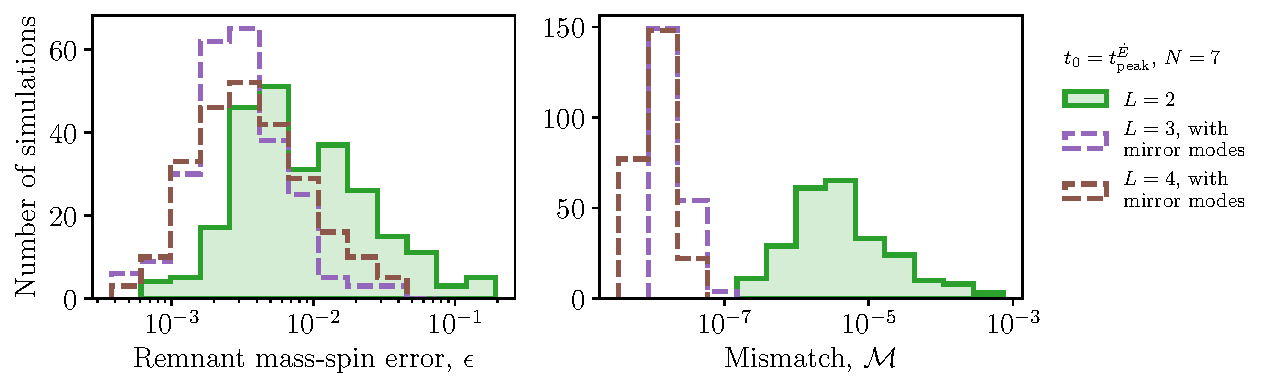
\includegraphics[width=\columnwidth]{ModellingTheRingdownFromPrecessingBlackHoleBinaries/misaligned_spin_epsilon_M_hist_harmonics.pdf}
    \caption[Remnant error and mismatches for fits to misaligned-spin SXS simulations using the harmonic model]{Left: histograms of the mass-spin remnant error $\epsilon$ from harmonic model fits (Eq.~\ref{full_ringdown}) to same 252 misaligned-spin SXS simulations used in Fig.\ref{misaligned_spin_epsilon_hist}. Shown (in dashed lines) are the $N=7$, $L=3$ and $L=4$ models with mirror modes. Also shown in green is the overtone model with $N=7$ and $L=2$ (no mirror modes); this is the same as the green histogram in Fig.~\ref{misaligned_spin_epsilon_hist} and is included here to aid comparison. Right: histograms of the mismatch from a fit with the true remnant mass and spin parameters, with the same models and SXS simulations as in the left histogram. The harmonic model, which includes many free parameters, achieves small mismatches but without significant improvement in the remnant error. We note that the inclusion of $L=4$ does not bring any additional improvements over $L=3$.}
    \label{misaligned_spin_epsilon_hist_harmonics}
\end{figure*}

To investigate whether the choice of ringdown start time could be contributing to the wider histograms seen in Figs.~\ref{misaligned_spin_epsilon_hist} and \ref{misaligned_spin_epsilon_hist_m10}, the behaviour of the mismatch heat maps (e.g.\ Figs.~\ref{305_epsilon_grid}, \ref{1856_epsilon_grid}, \ref{1856_mirror_mode_epsilon_grid}) with varying start time was explored for selected SXS simulations. 
Animations of ringdown fits with varying start time can be found at \cite{finch_eliot_2021_4538194}.
For the aligned-spin simulation SXS:BBH:0305, we see that the location of the mismatch minimum in the mass-spin plane settles on the true remnant properties for a sufficiently late choice of the start time ($t_0 \geq t_{\mathrm{peak}}^{h_{22}}$ for the $N=7$ overtone model). 
In addition, the mismatch minimum stays centred on the true remnant properties until numerical noise takes over.
For earlier choices of the start time, the $N=7$ overtone model gives biased values for the final mass and spin, see \cite{finch_eliot_2021_4538194}.
Applying the $N=7$ overtone model to the misaligned-spin simulation SXS:BBH:1856, we see that the location of the mismatch minimum moves around the mass-spin plane as start time is varied. Even at late times, it never settles on the true remnant properties.
The inclusion of mirror modes, as seen in Fig.~\ref{1856_mirror_mode_epsilon_grid}, narrows the mismatch minimum. The movement of the mismatch minimum around the mass-spin plane is reduced as well, however it still doesn't settle on the location of the true remnant properties.
This behaviour may explain some of the observed widening of the histograms, and perhaps hints something is missing from the ringdown model.


\subsection{Higher Harmonics}\label{kitchen-sink}

As demonstrated by Fig.~\ref{misaligned_spin_epsilon_hist} (and also Fig.~\ref{misaligned_spin_epsilon_hist_m10} in appendix \ref{appendix_a}), the overtone and mirror mode models considered so far achieve median values for the remnant error $\epsilon \sim 0.01$, a factor of 10 or more higher than the aligned-spin fits of Fig.~\ref{aligned_spin_epsilon_hist}. In addition, the spread of $\epsilon$ values recovered is significantly larger, leading to values of $\epsilon$ up to $\sim 0.1$. 
These models perform significantly worse in some cases for precessing systems than aligned-spin systems.

We now investigate whether the inclusion of higher harmonics (that is, QNMs with $\ell > 2$) can improve the fits to $h'_{22}(t)$.
These higher harmonics were neglected by both the overtone (Eq.~\ref{GieslerRD}) and mirror mode (Eq.~\ref{mirror_ringdown}) models.
However, mode mixing does occur as a consequence of the different angular basis functions used in the waveform decompositions in Eqs.~\ref{YlmExpansion} and \ref{general_ringdown} and the fact that these basis functions are not mutually orthogonal \cite{Berti:2014fga}.
The amount of mode mixing between the spherical mode ${}_{-2}Y_{\ell m}$ and the spheroidal mode ${}_{-2}S_{\ell m n}$ is determined by the remnant spin $\chi_f$ and the QNM frequency. This can be quantified by how much these functions fail to be orthogonal; i.e.\ by the integral
\begin{align}
     \mu_{\ell m, \ell' m' n'} = \delta_{mm'}\int_{\Omega} {}_{-2}Y_{\ell m}(\Omega)  ~ {}_{-2}S^*_{\ell ' m' n'}(\Omega) ~ \dd{\Omega},
\end{align}
where $\Omega$ denotes the angles $\theta,\,\phi$.
A translational offset between the NR and ringdown frames (e.g.\ due to a kick) can also lead to mixing between $m$-modes \cite{Boyle:2015nqa}; this effect is neglected here.
To include the contribution from higher harmonics, we define a new ringdown model for the spherical harmonic modes which now allows for a sum over different $\ell$:
\begin{align}\label{full_ringdown}
    h_{\ell m}^{N,\,L,\, {\rm mirror}}(t) = &\sum_{n=0}^N \sum_{l=2}^{L} \Big[ C_{l m n} e^{-i \omega_{l m n}(t-t_0)} \\ &+ C'_{l m n} e^{i \omega^*_{l m n}(t-t_0)} \Big]\quad \textrm{for} \quad t \geq t_0. \nonumber
\end{align}
This \emph{harmonic} model contains all of the allowed QNMs in Eq.~\ref{general_ringdown}, including the mirror modes and the overtones.
This comes at the expense of a large number of free parameters; there are $4(N+1)(L-\ell+1)$ in the complex amplitudes, plus the two remnant parameters $M_f,\; \chi_f$ that determine the complex QNM frequencies.

Multiple variations of this harmonic model were trialled (varying $N$, $L$, and the inclusion of mirror modes) on the same population of 252 misaligned-spin SXS simulations.
Fig.~\ref{misaligned_spin_epsilon_hist_harmonics} shows the chosen subset of results, which includes the $N=7$, $L=3$ and $L=4$ models (both with mirror modes). As before, we fit to the rotated $h'_{22}(t)$ spherical harmonic mode.
To make a clear comparison with the previous models, we again use a ringdown start time corresponding to the peak of the GW energy flux.

The inclusion of higher harmonics (dashed histograms in Fig.~\ref{misaligned_spin_epsilon_hist_harmonics}) drastically improves the mismatch.
A small mismatch is not surprising for a model with so many free parameters, and in some of these cases we are likely pushing beyond the limits of accuracy of the NR simulations. See appendix \ref{NR_error_appendix} for a discussion of the numerical errors.
There is a modest reduction in $\epsilon$ for some systems, and in particular we see less systems with $\epsilon > 0.01$ (at least for $L=3$). This hints at the importance of higher harmonics in some precessing systems. Despite this, we still see worst-case values of $\epsilon \sim 0.04$.


\section{Surrogates}\label{surrogate-section}

NR simulations are computationally expensive, and although the number of simulations available in public catalogs is growing they are still limited in their parameter space coverage. 
NR surrogate models \cite{Blackman:2015pia, Blackman:2017pcm, Varma:2019csw, Varma:2018mmi} would appear to be an attractive alternative.
These models use reduced-order and surrogate modelling techniques to extend the results of a set of NR simulations smoothly across parameter space. 
The use of surrogates could, in principle, allow us to extend the results of the previous section to include many more systems as well as allowing us to study how the excitations of the various QNMs vary during a smooth exploration of parameter space.
However, care must be taken as the surrogate modelling necessarily introduces an additional source of error into the waveforms, on top of the errors originally in the NR waveforms themselves.
 
When attempting to fit QNM ringdown models with overtones to NRSur7dq4 \cite{Varma:2019csw} waveforms, it was found that incorrect values for $M_f$ and $\chi_f$ were being recovered (particularly at high mass ratios). This being the case even for aligned-spin or non-spinning systems. Although the NRSur7dq4 waveforms do not provide the remnant properties, these can be obtained via NRSur7dq4Remnant \cite{Varma:2019csw} (it was found the problem did not lie with the values returned by NRSur7dq4Remnant but rather with the waveform surrogate).

\begin{figure}[b]
    \centering
    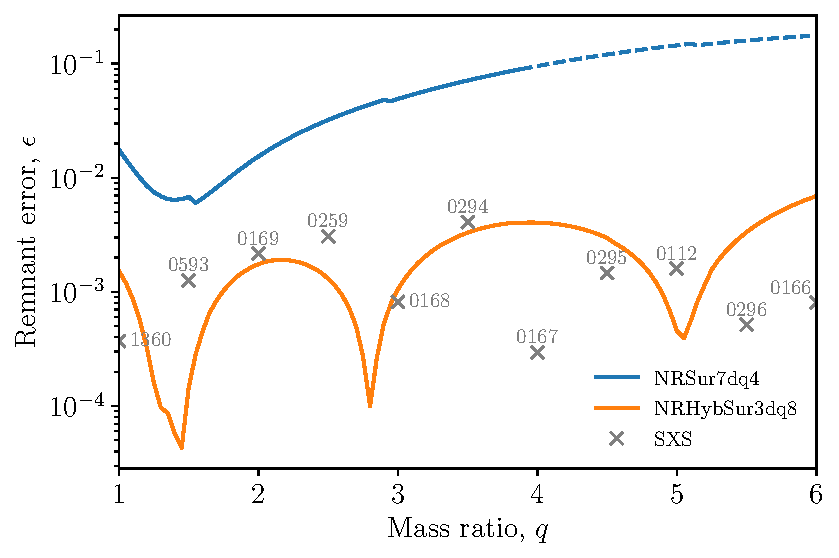
\includegraphics[width=0.8\columnwidth]{ModellingTheRingdownFromPrecessingBlackHoleBinaries/surrogate_epsilon_and_mass_ratio.pdf}
    \caption[Comparison of the error on measured remnant mass and spin from two surrogate models and a selection of SXS simulations.]{
    Comparison of the remnant error $\epsilon$ from two surrogate models and a selection of SXS simulations. All are zero initial spin. The fits were performed on the $h_{22}$ mode with the $N=7$ overtone model, Eq.~\ref{GieslerRD}, starting from the time of peak strain. The labels on each cross correspond to the SXS ID. The dashed line indicates where we are outside the training range of NRSur7dq4.
    }
    \label{surrogate_epsilon_vs_q}
\end{figure} 

To investigate the performance of NRSur7dq4 ringdown waveforms, a series of simulations with zero initial spin with increasing mass ratio $q$ from 1 to 6 were used. 
The $N=7$ overtone model (Eq.~\ref{GieslerRD}) was fitted to the $h_{22}(t)$ mode of each starting from the peak strain (as in section \ref{aligned-spin-section})
and the remnant error $\epsilon$ (Eq.~\ref{eq:epsilon}) was calculated for each.
The results are shown in Fig.~\ref{surrogate_epsilon_vs_q}, along with the results for similar fits performed directly on 11 zero-spin SXS simulations at discrete values of the mass ratio. 
The fits to the NRSur7dq4 surrogate produce values for $\epsilon$ that are 1-2 orders of magnitude higher than for the equivalent SXS simulations. 
Also shown are the results from a similar analysis with the more restrictive aligned-spin surrogate NRHybSur3dq8 \cite{Varma:2018mmi}; this was found to be in close agreement with the SXS simulations.

Residuals and mismatches can also be computed between surrogate and NR waveforms (taking care to align the waveforms in both time and phase).
For SXS:BBH:0168, the $q=3$, zero-spin simulation used in Fig.~\ref{surrogate_epsilon_vs_q}, we find $\sim 2\%$ residuals in the ringdown when comparing to the NRSur7dq4 surrogate with the same parameters. 
This leads to a mismatch between the surrogate and SXS:BBH:0168 of $3.7 \times 10^{-4}$, when integrating over the ringdown. For comparison, we have a $\sim 10^{-6}$ mismatch between the ringdown model Eq.~\eqref{GieslerRD} and the SXS simulation. The relatively high mismatch between the NRSur7dq4 and SXS waveforms translates to the relatively high values of $\epsilon$ seen in Fig.~\ref{surrogate_epsilon_vs_q}. 

It seems that the high-dimensional precessing surrogate NRsur7dq4 is not yet sufficiently accurate in the ringdown for the purposes of QNM overtone studies that, by virtue of their large number of free parameters, fit the ringdown with very small mismatches. 
By contrast, the lower-dimensional aligned-spin surrogate NRHybSur3dq8 does appear to be sufficiently accurate for such studies.


\section{Discussion} \label{sec:discussion}

This paper has made a first systematic attempt at using QNMs to model the ringdown of BHs formed from BBHs with misaligned component spins in the inspiral.
Previously, for aligned-spin systems, it has been found that the ringdown can be modelled with low mismatch and low remnant errors using a model that includes overtones of the fundamental QNM \cite{Giesler:2019uxc}. For seven overtones, the ringdown can be reliably modelled from the peak of the $h_{22}(t)$ strain for a range of SXS simulations.
Additionally, the inclusion of mirror modes can allow the ringdown to be modelled from even earlier times \cite{Dhani:2020nik}.
In this paper, which generalised these studies to precessing systems, we find that while QNM models can reliably achieve small mismatches, in the worst cases the remnant errors are more than a factor of 10 higher.
This is the case even when choosing to start the ringdown at the more conservative (i.e.\ later) peak in GW energy flux. 
The inclusion of higher harmonics reduces the remnant error in some cases, perhaps a sign that mode mixing in the ringdown is generally more important in precessing systems. However, in other cases, a bias remains in the recovered remnant properties.
We conclude that it is not possible to reliably model the ringdown from the peak in the flux, or indeed from the peak in the strain. 

We end by sounding a brief note of caution to any who attempt to construct a QNM model starting at or before the peak flux or strain. 
While such a model will work in some cases, it risks biased results in others. 
This risk is subtle because QNM models can give small mismatches even when they fail to adequately describe the remnant.


\section{Overtone Model Fits to a Variety of Precessing NR Simulations}\label{appendix_a}

\begin{figure}[h]
    \centering
    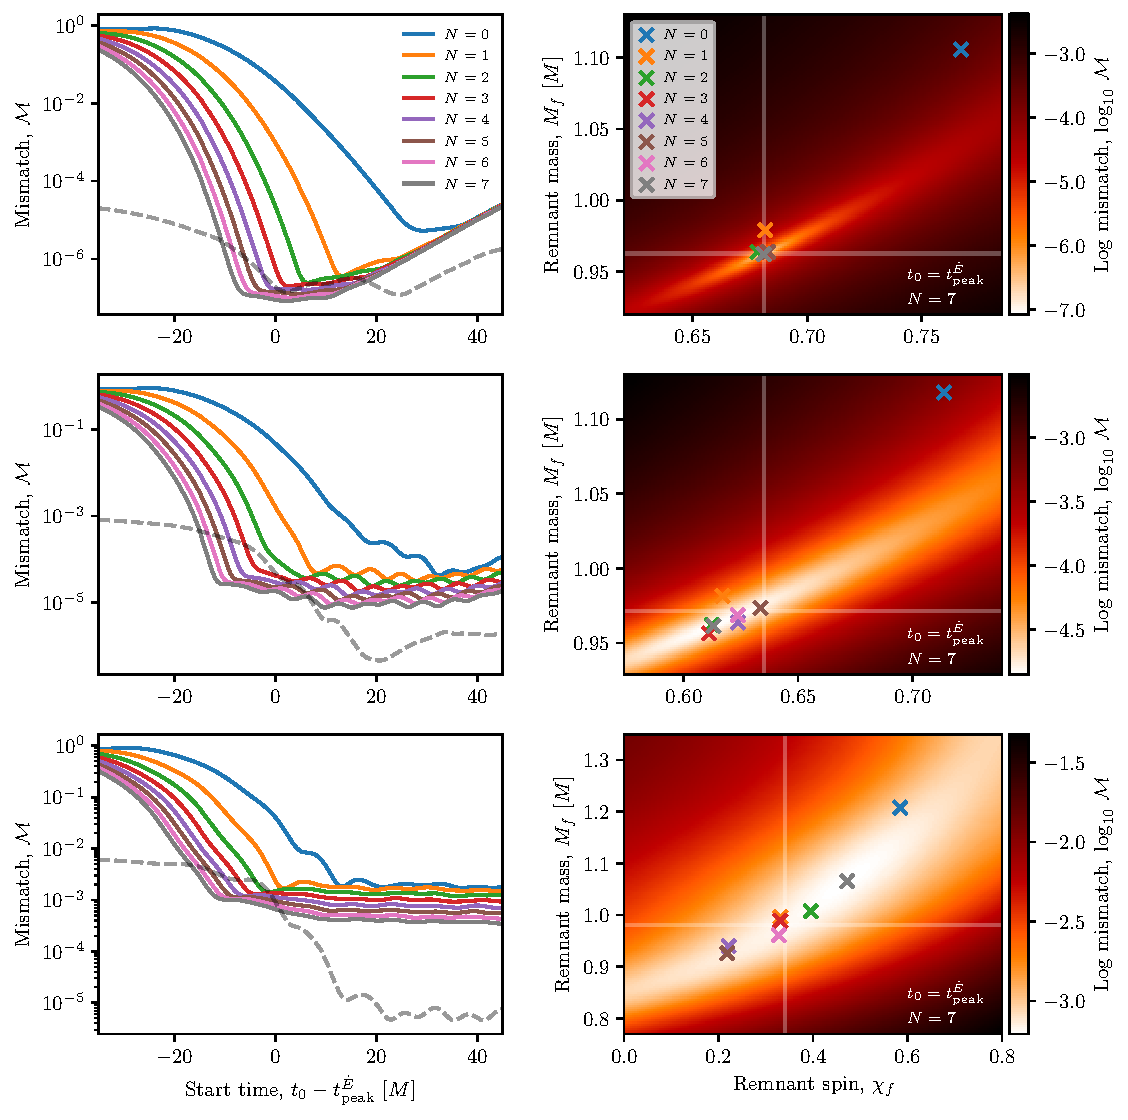
\includegraphics[width=\textwidth]{ModellingTheRingdownFromPrecessingBlackHoleBinaries/appendix_plot_with_error_edit.pdf}
    \caption[Selection of results for modelling the ringdown of misaligned-spin SXS simulations using the overtone model]{ 
    A selection of results for modelling the ringdown of precessing NR simulations from the SXS catalog \cite{Boyle:2019kee, Mroue:2013xna,sxs_catalog} using the overtone model in Eq.~\ref{GieslerRD}.
    These plots show the results for the three systems described in the table that have been chosen to illustrate the wider range of behaviours that occur for precessing systems, from good at the top to bad at the bottom.
    The left-hand column of plots also shows the difficulty in identifying a general start time for the ringdown as mismatch is minimised for a range of different times and sometimes there isn't even a clear first minimum.
    }
	\label{misaligned_spin_variation}
\end{figure}

\begin{footnotesize}
\begin{center}
\begin{tabular}{ c|c|c|c|c|c } 
%\hline
$\;$SXS:BBH ID $\;$ & $\;$Figure row$\;$ & $\;$Remnant error $\epsilon$$\;$ ($\epsilon_{\mathrm{NR}}$) &  $\;$Mass ratio $q$$\;$ & Component spins $\vb*{\chi}_1$, $\vb*{\chi}_2$  & $\;$Remnant spin $\vb*{\chi}_f$$\;$ \\
\hline
1677 & top & $8.1 \cross 10^{-4}$ ($1.8 \cross 10^{-4}$) & 2.64 & $(-0.06,\,0,\,0.27)$, $(-0.49,\,-0.55,\,0.06)$ & $(-0.05,\,0,\,0.68)$ \\ 
%\hline
1768 & middle & $2.6 \cross 10^{-2}$ ($8.0 \cross 10^{-4}$) & 3.49 & $(0.65,\,0.03,\,0.01)$, $(-0.3,\,0.05,\,0.47)$ & $(0.31,\,-0.02,\,0.56)$ \\ 
%\hline
1789 & bottom & $1.6 \cross 10^{-1}$ ($4.8 \cross 10^{-4}$) & 3.72 & $(0.46,\,0.08,\,-0.52)$, $(-0.43,\,-0.28,\,-0.17)$ & $(0.14,\,0.01,\,0.31)$ \\ 
%\hline
\end{tabular}
\end{center}
\end{footnotesize}


\section{Overtone Model Fits to a Population of Precessing NR Systems Starting Before the Peak Flux}\label{misaligned_spin_fits_appendix}

The analysis on the population of misaligned-spin simulations performed in section \ref{misaligned-spin-section} (results plotted in Fig.~\ref{misaligned_spin_epsilon_hist}) is repeated here using an earlier start time for the ringdown: $t_0=t^{\dot{E}}_{\rm peak}-10M$.
This was done to check whether a poor choice of start time was responsible for some of the poor fits obtained using the overtone model in Eq.~\ref{GieslerRD}.
The new results are plotted in Fig.~\ref{misaligned_spin_epsilon_hist_m10}.
We find that the $N=7$ model results do not significantly change with the new start time.
The $N=3$ and $N=0$ model results do change and generally give a worse fit with the earlier start time, as might be expected. This analysis shows that the overtone model (with or without mirror modes) cannot be reliably applied to precessing systems at early times. 

\begin{figure*}[h]
    \centering
    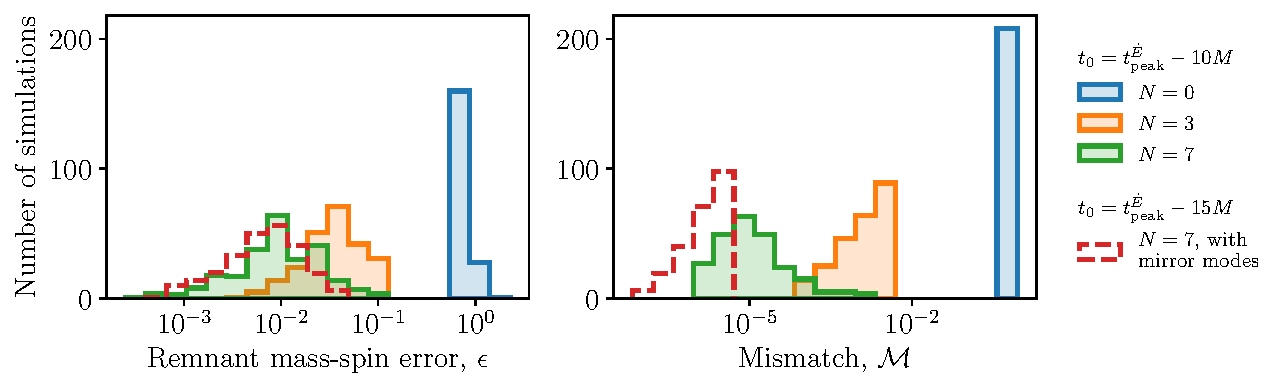
\includegraphics[width=\columnwidth]{ModellingTheRingdownFromPrecessingBlackHoleBinaries/misaligned_spin_epsilon_M_hist_m10.pdf}
    \caption[Remnant error and mismatches for fits to misaligned-spin SXS simulations using the overtone model starting from $10M$ before the peak of the $h_{22}$ strain]{
    Left: histograms of the mass-spin remnant error $\epsilon$ from an overtone model fit to the rotated $h'_{22}$ mode of 252 misaligned-spin SXS simulations for several different overtone numbers $N$. 
    Right: histograms of the mismatch from a fit with the true remnant mass and spin parameters, with the same overtone models and SXS simulations as in the left histogram.
    %
    These results are similar to those in Fig.~\ref{misaligned_spin_epsilon_hist} in the main text, but use a start time that is earlier by $10M$.
    %
    The solid histograms show results from fits performed starting $10M$ before the peak of the energy flux with $N$ overtones of the fundamental $\ell = m = 2$ mode.
    The red dashed line shows results from a $N=7$ model that also includes mirror modes and was fitted with a ringdown starting $15M$ before the peak in the energy flux.
    }
    \label{misaligned_spin_epsilon_hist_m10}
\end{figure*} 


\section{Numerical Relativity Errors}\label{NR_error_appendix}

It is important to remember the finite accuracy of the NR simulations used in ringdown studies.
This is particularly true when using models with many QNMs which, by their very nature, use a large number of free parameters and regularly achieve very small ($\sim 10^{-6}$) mismatches.
If care is not taken, we risk fitting our models to the numerical noise. 
In this appendix we describe the numerical checks performed on the 5 individual simulations used in this paper: SXS:BBH:0305, 1856, and the three simulations shown in Fig.~\ref{misaligned_spin_variation}.
In each case the numerical errors were estimated by comparing results obtained using data from the two highest resolutions (levels) available in the SXS catalog. 

First, we quantify the numerical error in the mismatch.
This was done by calculating the mismatch between the two NR resolutions from a time $t_0$ to a time $T = t_0 + 100M$, for a range of $t_0$. For each start time, we optimally align the two waveforms in time (taking the absolute value in the mismatch automatically optimises the mismatch over phase). The alignment in time can be done by matching the time of peak strain, for example, or by numerically rolling the waveform to find the optimal time shift for each mismatch calculation.
The results are shown by the grey dashed lines in the mismatch vs start time plots in Figs.~\ref{305_mismatch_vs_t0}, \ref{1856_mismatch_vs_t0} (duplicated in Fig.~\ref{1856_mirror_mode_mismatch_vs_t0}) and the 3 panels of Fig.~\ref{misaligned_spin_variation}.
Generally, we see numerical error estimates at or below the model mismatches, particularly at late times, indicating that we are not fitting to the numerical noise.
The main exception is Fig.~\ref{1856_mirror_mode_mismatch_vs_t0} where the mirror mode model is applied to a precessing system. This is expected; precessing NR simulations, and those with high mass ratios are generally expected to have larger numerical errors. Additionally, the mirror mode and harmonic models have the highest numbers of free parameters making them more likely to reach the accuracy of the NR simulation. 

Second, we investigate the numerical error on the remnant mass and spin.
We quantify the numerical error with $\epsilon_{\mathrm{NR}}$, the Euclidean distance (Eq.~\ref{eq:epsilon}) between the remnant properties reported in the two highest resolution levels of the NR simulation.
The $\epsilon_{\mathrm{NR}}$ values are reported in the main text and in the table in appendix \ref{appendix_a}.
In all cases $\epsilon_{\mathrm{NR}} < \epsilon$. This supports the conclusions in the main text and indicates they are likely to be robust against numerical noise in the underlying NR simulations used.
 
% Chapter 3

\chapter{Frequency-domain Analysis of Black-hole Ringdowns}

\label{Chapter3}

\section{Introduction}\label{ch3:sec:introduction}

A key motivation of the NR ringdown studies discussed in the previous chapter is to understand what to expect from nature. 
This is the subject of the next two chapters: testing our expectations with real GW data.

As discussed in the previous chapter, theoretical studies using catalogs of BBH simulations suggest the ringdown typically starts early in the merger process, i.e.\ at or even slightly before the time of peak strain amplitude. 
This is only possible if the ringdown modelling includes overtones ($n \geq 1$), and possibly a combination of mirror modes and/or higher harmonics ($\ell \geq 3$).
This early start time is good for the prospects of observing QNMs because it means the signal amplitude is still large when the ringdown starts and consequently the SNR in the ringdown is large.

Once QNMs have been correctly identified in an observed signal, they provide an exciting opportunity for testing GR, the Kerr metric hypothesis, and the no-hair theorem. 
The idea of using QNM frequencies for such tests predates the detection of GWs, and so experimental QNM tests of GR started immediately with the first GW observation.
% Ref.~\cite{LIGOScientific:2016lio} found that the data following the peak of GW150914 was consistent with the least-damped QNM of the expected remnant.
% Subsequently, several groups reanalysed the ringdown of GW150914 with the aim of identifying additional QNMs for use in spectroscopic tests~\cite{Carullo:2019flw, Isi:2019aib, Brito:2018rfr}. 
% With the second and third GW catalogs, similar analyses are now routinely performed on all suitable events~\cite{LIGOScientific:2020tif, LIGOScientific:2021sio}.
Despite the difficulties discussed in Section~\ref{ch1:sec:limitations}, detecting and characterising QNMs is a key goal in GW astronomy. 
GW data analysis is almost universally performed in the frequency domain, where it is most natural to characterise the noise.
To satisfy the periodicity requirements of the Fourier transform and avoid spectral leakage, the data is windowed before and after the GW signal.
However, to perform a ringdown-only analysis, a sharp cut must be applied in the time domain to isolate the ringdown signal. 
Applying any window functions would suppress the ringdown signal, or (if the analysis data is extended to earlier times) the inspiral-merger would contaminate the analysis.
See Ref.~\cite{Isi:2021iql} for a discussion.
This problem can be solved by instead working in the time domain, where the ringdown can be isolated cleanly from a chosen start time, $t_0$, and the noise is instead characterised by a non-diagonal covariance matrix.
However, as the particular segment of data to be analysed is chosen before the analysis begins, the ringdown start time (and consequently the source sky location) usually must be fixed in these analyses. 
Another drawback of working in the time domain is that, as the noise covariance matrix is no longer diagonal, the computational cost of the likelihood is increased. 
The covariance matrix is constructed with the autocovariance function, which characterises the noise in the time domain.
And, as discussed in Ref.~\cite{Isi:2021iql}, care must be taken when estimating the autocovariance to avoid corrupting the ringdown data. 
Therefore, there are additional subtleties in a time-domain analysis compared to a frequency-domain analysis.

This time-domain approach is not the only way to formulate a robust ringdown analysis.
Ref.~\cite{Capano:2021etf} proposed an alternative approach which is expressed in the frequency domain, but uses a modified form of the likelihood (involving ``in-painting'' the data before the start of the ringdown in such a way as to remove its contribution to the likelihood).
However, it has been shown that this method is formally equivalent to the standard time-domain approach~\cite{Isi:2021iql} and suffers from the same limitations.
It should also be noted that Ref.~\cite{Capano:2021etf} applied their method to GW190521, where a higher harmonic was identified in the ringdown.
This finding is apparently in contradiction with the earlier results of Ref.~\cite{LIGOScientific:2020tif}, which use a time-domain approach.
That these two formally equivalent analyses~\cite{LIGOScientific:2020tif, Capano:2021etf} can come to different conclusions regarding the QNM content of GW190521 highlights some of the difficulties that come with this type of analysis, where important choices (that can affect the result) for the ringdown start time have to be made and care must be taken with the noise estimation.

Another approach~\cite{Brito:2018rfr} is to make use of the full GW signal, and perform the analysis with augmented effective-one-body~\cite{Buonanno:1998gg} waveforms.
By calibrating QNM amplitudes with NR simulations, QNM frequencies can be measured.
An additional QNM ``frequency-filter'' method has also been proposed~\cite{Ma:2022wpv}, which targets particular QNMs and removes them from the data.
How consistent the remaining data is with noise can be used to infer remnant properties without requiring any knowledge of the QNM amplitudes, and to estimate when the linear ringdown regime begins.
These approaches are a valuable way of investigating the QNM content of GW data. 
But, although advantageous in some ways, the lack of measurements on QNM amplitude means there is one less way to quantify the presence of the modes.
The latter QNM filter method requires a fixed sky location in order to align data from multiple detectors.

In this chapter, we present a new approach to performing ringdown analyses in the frequency domain. 
We employ a flexible sum of truncated wavelets to model the inspiral-merger signal (inspired by \textsc{BayesWave}~\cite{Cornish:2014kda, Cornish:2020dwh}) and QNMs to model the ringdown.
The general idea behind our approach is illustrated in Fig.~\ref{fig:demo}.
By working in the frequency domain, we can use the standard, and now very mature, GW data analysis pipelines (our analysis pipeline borrows from the public \textsc{Bilby} package~\cite{Ashton:2018jfp}).
Also, working in the frequency domain makes it trivial to search and marginalise over the sky position the ringdown start time, $t_0$. 
We hope this approach can complement existing time-domain analyses.
The code associated with this work is available at Ref.~\cite{fdringdown}, and a complete set of posterior samples from this work are made available at Ref.~\cite{finch_eliot_2021_5569759}.

\begin{figure}[t!]
    \centering
    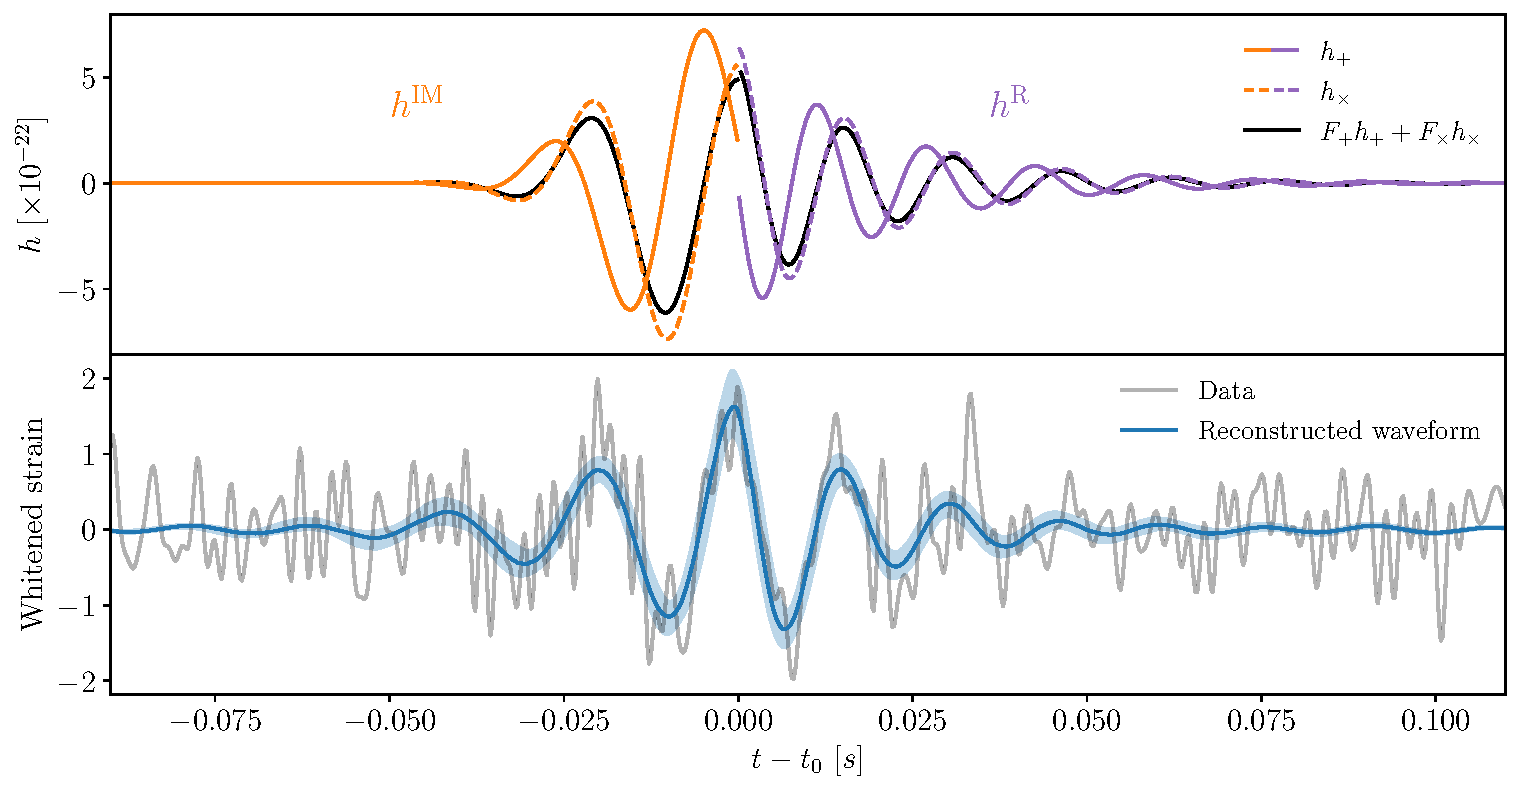
\includegraphics[width=0.9\columnwidth]{FrequencyDomainAnalysisofBlackHoleRingdowns/demo.pdf}
    \caption[Illustration of the frequency-domain ringdown analysis method]{ 
    This figure is intended to illustrate the idea behind our approach for analysing the ringdown in the frequency domain.
    The grey line in the bottom panel shows the whitened and band-passed Livingston time-series data around GW190521. % ; this loud GW signal comes from a high-mass BBH merger and exhibits a clear ringdown.
    For the purpose of illustration, we use the simplest version of our model where a single, truncated sine-Gaussian wavelet is used to model the inspiral-merger part of the signal and the fundamental $\ell=m=2$, $n=0$ QNM is used to model the ringdown.
    The ringdown start time, $t_0$, is allowed to vary as part of a Bayesian analysis which also searches over different values of wavelet parameters, the source sky position, the QNM amplitude and phase, and over the remnant BH mass and spin. 
    Full details of this analysis will be presented elsewhere.
    The top panel shows the maximum likelihood waveform broken down into its wavelet ($h^{\rm IM}$, orange) and ringdown ($h^{\rm R}$, purple) parts as well as into plus (solid) and cross (dashed) polarisations. 
    The discontinuity in our model can be clearly seen in the coloured lines. 
    However, when these polarisations are combined and projected (see Eq.~\ref{eq:projection_antenna}) onto the interferometer (black line) the result is nearly continuous; we emphasise that this continuity has not been imposed by the model but is rather ``learnt'' from the data. When the projected maximum likelihood waveform is whitened according to the detector noise curve it becomes completely continuous, this is plotted as the central blue line in the bottom panel.
    In the bottom panel we also plot the uncertainty (90\% credible region; blue shaded band) on the recovered signal.
    }
    \label{fig:demo}
\end{figure}

The details of our method are described in Section~\ref{sec:methods}, where we compare and contrast the time- and frequency-domain likelihood functions before introducing our frequency-domain approach.
In Section~\ref{sec:injection_study} we present the results of a series of analyses on simulated GW signals where we test the performance of our approach and compare it with time-domain methods.
We present our conclusions in Section~\ref{ch3:sec:discussion}.
A complete set of posterior samples from this work are made available at Ref.~\cite{finch_eliot_2021_5569759}.


\section{Methods}\label{sec:methods}

This section describes the details of the proposed frequency-domain approach to the analysis of BH ringdowns. 
Section~\ref{subsec:data_analysis} describes the GW likelihood function and its implementation in both the time and frequency domains.
Section~\ref{subsec:motivation} motivates our frequency-domain approach by describing an extreme limit in which it becomes equivalent to the standard, time-domain approach.
Finally, Section~\ref{subsec:model} describes the combination of truncated wavelets and QNMs that comprise our waveform model.


\subsection{Time- and frequency-domain likelihoods}\label{subsec:data_analysis}

Most GW data analysis is done in the frequency domain because, with the usual assumptions of stationary zero-mean Gaussian noise, the instrumental noise is fully described by the (one-sided) noise power spectral density (PSD), $S_n(f)$.
In the literature, the most commonly encountered expression for the log-likelihood in one interferometer is the integral
\begin{align} \label{eq:logL_FD_continuous}
	\log\mathcal{L}(d|\pvec{\theta}) = -2\int_{0}^{\infty}\!\mathrm{d}f\;\frac{|\tilde{d}(f)-\tilde{h}(f;\pvec{\theta})|^2}{S_n(f)} + \mathrm{norm},
\end{align}
where $d(t)$ is the observed data, and $h(t;\pvec{\theta})$ is the signal model (projected onto the interferometer) described by parameters $\pvec{\theta}$.
The normalisation constant in the likelihood is unimportant for our purposes and will be dropped in all following equations.
A tilde denotes the Fourier transform of a time series.
Because the noise is uncorrelated between two well separated interferometers, the log-likelihood for a network is obtained by summing the independent contributions from each instrument.

In practice, it is necessary to work with discretely sampled time series; $d_j = d(t_j)$, where $t_j=j\delta t$ for $j=0,1,\ldots, J-1$, and where $1/\delta t$ is the sampling frequency.
The discrete Fourier transform $\tilde{d}_k = \tilde{d}(f_k)$ is sampled at (positive) frequencies $f_k=k/(J\delta t)$ for $k=0,1,\ldots,K-1$, where $K=\left \lfloor (J+2)/2\right \rfloor$.
The log-likelihood in terms of the discretely sampled frequency series is given by the following sum,
\begin{align} \label{eq:logL_FD_discrete}
	\log\mathcal{L}(d|\pvec{\theta}) = \frac{-2}{J\delta t}\sum_{k}\frac{|\tilde{d}_k-\tilde{h}_k(\pvec{\theta})|^2}{S_n(f_k)},
\end{align}
which can be compared to Eq.~\ref{eq:logL_FD_continuous}.
The noise PSD is usually estimated from off-source data using a Welch periodogram~\cite{1161901}.
The frequency-domain expression for the log-likelihood involves a single sum; the noise covariance matrix is diagonal in the frequency domain.
Although, for finite duration time series there can be small correlations between frequency bins~\cite{Talbot:2021igi}.

The log-likelihood can also be expressed in the time domain via
\begin{align} \label{eq:logL_TD_discrete}
	\log\mathcal{L}(d|\pvec{\theta}) = -\frac{1}{2}\sum_{jj'}\qty[d_j-h_j(\pvec{\theta})] C^{-1}_{jj'} \qty[d_{j'}-h_{j'}(\pvec{\theta})],
\end{align}
where $C_{jj'}$ is the noise covariance matrix.
The time-domain expression for the log-likelihood involves a double sum over a dense covariance matrix which is computationally more costly to evaluate than the frequency-domain expression [$\mathcal{O}(J^2)$ as opposed to $\mathcal{O}(J)$].

Because the noise is assumed to be stationary, $C_{jj'}$ has the Toeplitz structure
\begin{align} \label{eq:Toeplitz}
	C_{jj'} = \rho_{|j-j'|},
\end{align} 
where $\rho_j$ is the noise autocovariance. 
This can also be estimated from off-source data using the following two-point expectation:
\begin{align} \label{eq:autocovariance}
	\rho_j = \frac{1}{\mathcal{J}}\sum_{j'=0}^{\mathcal{J}-1}n_{j'}n_{(j'+j)}.
\end{align}
Here, $\mathcal{J}$ is the length of some off-source data segment, which is usually chosen to be longer than the analysis data (i.e.\ $\mathcal{J} \gg J$)~\cite{Isi:2021iql}.
It is also necessary to treat the ``edges'' of the data segment (i.e.\ where $j + j' > \mathcal{J}-1$) either by zero-padding or imposing periodicity: $\rho_j = \rho_{\mathcal{J}-j}$.
Although these different treatments result in an autocovariance that differs for large $j$, if $\mathcal{J}$ is sufficiently large then the autocovariance will be consistent for $j < J$ (which is what enters the calculation of the likelihood).

The two expressions for the log-likelihood are equivalent.
The noise autocovariance (which appears in the time-domain log-likelihood) is related to the PSD (in the frequency-domain log-likelihood) via a discrete Fourier transform (Wiener-Khinchin theorem), when imposing the circularity condition~\cite{Isi:2021iql}:
\begin{align} \label{eq:WKtheorem}
	\frac{1}{2}S_n(f_k) = \delta t \sum_{j}\rho_j \exp\left(\frac{-2\pi ijk}{J}\right).
\end{align}
We use the inverse of Eq.~\ref{eq:WKtheorem} to estimate the autocovariance, which comes with the requirement that the off-source segment length used in the PSD estimate is much longer than the analysis length~\cite{Isi:2021iql}.

The time-domain expression for the log-likelihood has hitherto been considered more suitable for ringdown analyses.
This is because in the time-domain expression no Fourier transform of the data or model is required, and so no periodicity has to be ensured.
The abrupt start of ringdown models means they do not satisfy this periodicity condition, which leads to spectral leakage upon Fourier transforming. 
When performing Fourier transforms of the GW data, periodicity is ensured by applying window functions to taper the data.
This makes it difficult to isolate the ringdown region of a GW signal in some data; a sharp cut at the ringdown start time would introduce a discontinuity, whereas a smooth window would either suppress the ringdown signal or risk contamination of the ringdown by including unwanted parts of the inspiral-merger (see Fig.~7 in Ref.~\cite{Isi:2021iql} for an illustration of this). These problems are naturally avoided in the time domain. 
In the following sections we describe how these problems can also be overcome in a frequency-domain analysis.


\subsection{Marginalising over the inspiral-merger}\label{subsec:motivation}

We now motivate our approach to analysing the ringdown by first discussing a special case in which it becomes formally equivalent to the standard time-domain approach. 

Consider first the case of a single interferometer.
The observed data is a discretely sampled time series:
\begin{align}
	\ldots,\ d_{-2},\ d_{-1},\ d_{0},\ d_{1},\ d_{2},\ \ldots
\end{align}
We assume that the ringdown has been identified as starting at the time of $d_0$.
The GW signal has a large amplitude around $d_0$, but decays to zero at early and late times.

The standard approach to analysing the ringdown is to cut the data at the start time where the signal amplitude is large and take only the data after that time (i.e.\ $d_{0},\ d_{1},\ d_{2},\ \ldots$) and to model this using a superposition of QNMs described by parameters $\pvec{\theta}$ (e.g.\ the remnant mass, spin, amplitudes and phases for each QNM).
The likelihood is written as
\begin{align} \label{eq:motivation_A}
	\mathcal{L}(d_{0}, d_{1}, d_{2}, \ldots|\pvec{\theta}),
\end{align}
and, because we have cut the signal where the amplitude is large, this must be expressed in the time domain (Eq.~\ref{eq:logL_TD_discrete}) to avoid problems of spectral leakage.

We could instead extend our analysis segment backwards by starting at $d_{-1}$, and then analyse this longer data stream with a new model that treats the value of the signal at $d_{-1}$ as being a completely free parameter. 
The model is otherwise unchanged at later times and is now described by parameters $(\hat{d}_{-1}, \pvec{\theta})$.
Note that the new model for $d_{-1}$ is entirely unphysical and is also discontinuous in the sense that there is no requirement that the model takes similar values at times $-1$ and 0.
The likelihood for this new model
\begin{align} \label{eq:motivation_B}
	\mathcal{L}(d_{-1}, d_{0}, d_{1}, d_{2}, \ldots|\hat{d}_{-1}, \pvec{\theta}),
\end{align} 
is also given by Eq.~\ref{eq:logL_TD_discrete}, only with a slightly larger covariance matrix.
If we marginalise this with respect to the ``inspiral-merger parameter'' $\hat{d}_{-1}$ 
(adopting a flat, improper prior on $\hat{d}_{-1}$ ranging between $\pm\infty$)
then we recover the original likelihood in Eq.~\ref{eq:motivation_A}, i.e.\
\begin{equation} \label{eq:motivation_C}
    \mathcal{L}(d_{0}, d_{1}, d_{2}, \ldots|\pvec{\theta}) = \int_{-\infty}^{\infty} \mathrm{d}\hat{d}_{-1}\; \mathcal{L}(d_{-1}, d_{0}, d_{1}, d_{2}, \ldots|\hat{d}_{-1}, \pvec{\theta}).
\end{equation}
This follows from well-known properties of the Gaussian distribution.

We can of course include more early-time data in a similar way. 
If we treat the value of the GW signal at each of the times $d_{-2},\ d_{-3},\ \ldots$ as free parameters and marginalise over all of them then we recover the original likelihood in Eq.~\ref{eq:motivation_A}.
The point of doing this is that it allows us to start the analysis at early times when the amplitude of the GW signal in the data is small.
This means we can apply windowing, aka tapering, operations to the data without fear of suppressing the signal, and we can therefore transform the likelihood into the frequency domain without encountering spectral leakage problems.

The extension of this argument to multiple interferometers is straightforward. 
The values of the model at each early time in each interferometer must all be treated independently as free parameters and marginalised over in the manner of Eq.~\ref{eq:motivation_C}.

The point we wish to emphasise is that an analysis of only the ringdown data (usually done in the time domain to avoid problems of spectral leakage) is equivalent to an analysis of all the data (which can be done in the frequency domain using standard GW data analysis techniques) if the inspiral-merger part of the signal is suitably marginalised out. 
This requires the use of an unphysical and discontinuous model for the inspiral-merger signal.
For the equivalence to be exact, the inspiral-merger model should include an extremely large number of free parameters (one for each time stamp in each interferometer), but we will argue below that in practice it is sufficient to use a smaller number of parameters provided a sufficiently flexible model is used.

This discussion motivates the model we describe in Section~\ref{subsec:model}. Once the likelihood is expressed in the frequency domain, several extensions of the analysis (such as treating the ringdown start time as a parameter of the model; see Section~\ref{subsec:t0}) become natural.


\subsection{Model}\label{subsec:model}

As it is clearly impractical to model the data at each time stamp as a free parameter, we propose to use a continuous (but very flexible) inspiral-merger model instead. 
We choose a sum of sine-Gaussian wavelets, which are then truncated at the ringdown start time and attached to a ringdown QNM model. 
With this method, we aim to model the full inspiral-merger-ringdown signal.

The ringdown model is zero for early times, and after a start time $t_0$ takes the form
\begin{equation}\label{ch3:eq:hr}
    h^\mathrm{R}(t) = h_+^\mathrm{R}(t) - ih_\times^\mathrm{R}(t) = \sum_{\ell m n} A_{\ell m n} e^{-i[\omega_{\ell m n}(t-t_0) - \phi_{\ell m n}]}, \quad t \geq t_0,
\end{equation}
where the complex QNM frequencies $\omega_{\ell m n} = 2\pi f_{\ell m n} - i/\tau_{\ell m n}$ are functions of the remnant BH mass $M_f$ and dimensionless spin magnitude $\chi_f$. Here, $f_{\ell m n}$ is the oscillation frequency, and $\tau_{\ell m n}$ is the damping time.
Each QNM is further described by an amplitude, $A_{\ell m n}$, and phase parameter, $\phi_{\ell m n}$. 
It is possible to analytically take the Fourier transform of this expression and thereby write the ringdown model in the frequency domain as
\begin{equation}
    \Tilde{h}^{\mathrm{R}}(f) = \int_{-\infty}^\infty \dd{t} \qty[h_+^\mathrm{R}(t) - ih_\times^\mathrm{R}(t)] e^{-2\pi i f t} = \sum_{\ell m n} \frac{A_{\ell m n} e^{-i[2\pi ft_0 - \phi_{\ell m n}]}}{i(\omega_{\ell m n} + 2\pi f)}.
\end{equation}

We model the inspiral-merger part of the signal as a truncated sum of $W$ wavelets.
The inspiral-merger model is zero for late times, but before the start time $t_0$ takes the form
\begin{align}
	h^\mathrm{IM}(t) &=  h_+^\mathrm{IM}(t) - ih_\times^\mathrm{IM}(t) \nonumber \\
	&= \sum_{w=1}^{W} \mathcal{A}_w \exp \Bigg[-2\pi i \nu_w(t-\eta_w) - \qty(\frac{t-\eta_w}{\tau_w})^2 + i\varphi_w \Bigg], \quad t < t_0.
\end{align}
The limit on time is equivalent to a model which is multiplied by a Heaviside step function, $H(t_0 - t)$. Each wavelet is described by five parameters: $\mathcal{A}_w$ and $\varphi_w$ are the wavelet amplitudes and phases, $\tau_w$ are the wavelet widths, $\nu_w$ are the wavelet frequencies, and $\eta_w$ are the wavelet central times. Again, it is possible to analytically take the Fourier transform of this expression and thereby write the inspiral-merger model in the frequency domain as
\begin{align}
	\Tilde{h}^\mathrm{IM}(f) &= \int_{-\infty}^\infty \dd{t} \qty[h_+^\mathrm{IM}(t) - ih_\times^\mathrm{IM}(t)] e^{-2\pi i f t} \\
	&= \sum_{w=1}^{W} \mathcal{A}_w \exp[-2\pi i\nu_w \eta_w -\pi^2(f+\nu_w)^2\tau_w^2 +i\varphi] \nonumber\\
	&\quad\times \frac{\sqrt{\pi}}{2}\tau_w \left(1 + \mathrm{erf} \left[ \frac{t_0-\eta_w}{\tau_w} + \pi i(f+\eta_w)\tau_w \right] \right).\nonumber
\end{align}

The full IMR model is simply given by
\begin{equation}
	h(t) = h^\mathrm{IM}(t) + h^\mathrm{R}(t).
\end{equation}
We refer the reader to Fig.~\ref{fig:demo}, which provides an illustration of this model with a single QNM and a single wavelet ($W=1$).

If $N$ QNMs are used, then the ringdown part of the model is described by $2N+2$ parameters.
The inspiral-merger part of the model is described by $5W$ parameters (these numbers do not include $t_0$).
Additionally, there are two sky position angles ($\alpha$ and $\delta$) and a polarisation angle ($\psi$) which enter the detector response described below.
Finally, the ringdown start time ($t_0$) can also be treated as a model parameter in our frequency-domain approach.
For a typical choice of these parameters, our IMR model is discontinuous at $t_0$.
The inspiral-merger part of the model contains no information of the physics of the source and no attempt is made to enforce continuity between the two parts; this helps to decouple the ringdown inference from the inspiral-merger parts of the data and thereby ensure that we are really performing a ringdown analysis. 

To complete the description of our model, the detector response is given by projecting the waveform polarisations onto each interferometer (IFO) with the appropriate antenna patterns, $F^\mathrm{IFO}_{+,\times}$.
For a given sky location and GW polarisation angle the detector response for each ${\mathrm{IFO}\in \{\mathrm{H}, \mathrm{L}, \mathrm{V} \}}$ is given by
\begin{equation} \label{eq:projection_antenna}
    h^\mathrm{IFO}(t) = F^\mathrm{IFO}_+(\alpha, \delta, \psi) ~ h_+(t + \Delta t_\mathrm{IFO}) + F^\mathrm{IFO}_\times(\alpha, \delta, \psi) ~ h_\times(t + \Delta t_\mathrm{IFO}).
\end{equation}
Here, $\Delta t_\mathrm{IFO}(\alpha, \delta)$ accounts for the different signal arrival times at the detectors and is also a function of sky location.
By definition, $h_+(t) = \Re\{ h(t) \}$, and $h_\times(t) = -\Im \{ h(t) \}$.
Note, the frequency-domain waveforms presented here are Fourier transforms of the complex polarisation sum $h_+(t) - ih_\times (t)$. This means the separation into the plus and cross polarisations is not as simple as for the time-domain waveforms. Instead, the property that $\Tilde{h}^*_{+,\times}(-f) = \Tilde{h}_{+,\times}(f)$ for a real time-series implies that
\begin{equation}
    \Tilde{h}_+(f) = \frac{\Tilde{h}(f) + \Tilde{h}^*(-f)}{2}, \quad \Tilde{h}_\times(f) = -\frac{\Tilde{h}(f) - \Tilde{h}^*(-f)}{2i}.
\end{equation}


\section{Injection study}\label{sec:injection_study}

We use the NR surrogate NRHybSur3dq8~\cite{Varma:2018mmi} to simulate the full inspiral, merger and ringdown signal from GW190521-like and GW150914-like sources. 
We use these two sources to test our frequency-domain approach on the analysis of the ringdown and compare the results with a standard, time-domain analysis.
Results from the GW190521-like analyses are shown here while the results from the GW150914-like analyses are shown in Section~\ref{app:GW150914}.

For all the GW190521-like injections, the surrogate was initialised with a total mass of $271\,M_\odot$ (all masses are given in the detector frame) and a mass ratio of $1.27$. 
For simplicity, all of the component spins were set to zero and the inclination angle was also chosen to be zero (i.e.\ the source was injected ``face-on'').
The simulated sky location and GW polarisation angle were taken to be the maximum likelihood values from the NRSur7dq4 analysis in Refs.~\cite{LIGOScientific:2020ibl, gwtc2datarelease} ($\alpha = 0.164$, $\delta = -1.14$, $\psi = 2.38$).
The distance to the binary was chosen so that it gives a particular value of the optimal SNR in Livingston; this was usually chosen to be 15 (corresponding to a distance of $4016\,\mathrm{Mpc}$) so that it would likely be possible to detect multiple QNMs (in particular overtones), but several smaller values are also considered in Section~\ref{subsec:overtones}.
We perform zero-noise injections (i.e. analysing simulated data with a noise realisation of zero) into a three-interferometer H-L-V LIGO-Virgo network (except in Section~\ref{subsec:t0} where a two-interferometer H-L injection is performed for comparison) and use the average PSDs from the first three months of O3 (available at Ref.~\cite{o3psd}).

Although an important advantage of our approach is that it allows for easy marginalisation over the source sky position and ringdown start time, we first apply it to the case where these are fixed. 
This allows us to compare our results more directly to those from a time-domain analysis.
The sky position and polarisation angles $\alpha$, $\delta$ and $\psi$ are fixed to their injected values and the ringdown start time $t_0$ is fixed to be $12.7\,\mathrm{ms}$ ($\sim 10\,M_f$ in geometric units) after the peak of the strain (this choice follows the analysis of the real GW190521 signal in Ref.~\cite{LIGOScientific:2020iuh}).

\begin{figure}[t!]
    \centering
    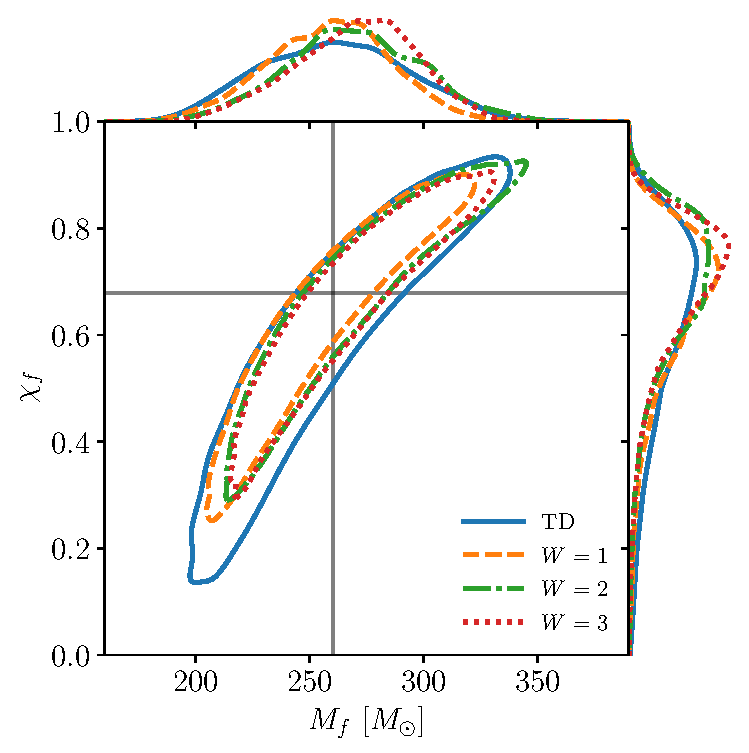
\includegraphics[width=0.6\columnwidth]{FrequencyDomainAnalysisofBlackHoleRingdowns/mass_spin_corner_fixed_sky.pdf}
    \caption[Posteriors on the remnant mass and spin for a GW190521-like injection analysed with a fixed sky location and ringdown start time, for different numbers of wavelets]{ 
    Posteriors on the (detector frame) remnant mass and dimensionless spin for the GW190521-like injection using a single QNM and analysed with a fixed sky position, GW polarisation angle and ringdown start time.
    The main panel shows the $90\%$ confidence contour while the side plots show the one-dimensional marginalised posteriors.
    The solid blue line shows the results of a time-domain (TD) analysis.
    The other dashed and dotted lines show the results of frequency-domain analyses using different numbers of wavelets, $W$.
    The vertical and horizontal lines indicate the true values.
    }
    \label{fig:mass_spin_corner_fixed_sky}
\end{figure}

First, for reference, an analysis using the time-domain expression for the log-likelihood was performed on this injection searching for the fundamental QNM (i.e.\ $\ell = m = 2$ and $n=0$).
Only the ringdown data $t\geq t_0$ was analysed; the time series in each interferometer was shifted to geocenter time using the injected sky position, then cut to include $0.1\,\mathrm{s}$ of data from the start of the ringdown.
For each interferometer, the PSD was converted into an autocovariance function using the inverse of the transformation in Eq.~\ref{eq:WKtheorem} and this was used to construct the covariance matrix with Eq.~\ref{eq:Toeplitz}.
We sample over the remnant mass ($M_f$, using a flat prior between $100\,M_\odot$ and $400\,M_\odot$), the dimensionless remnant spin ($\chi_f$, using a flat prior between $0$ and $0.99$), the QNM phase ($\phi_{220}$, using a flat, periodic prior between $0$ and $2\pi$), and the QNM amplitude ($A_{220}$, using a flat prior between 0 and $5 \times 10^{-21}$).
As modes beyond the fundamental will likely have amplitude posteriors consistent with zero, we use a flat prior (as opposed to a log-uniform prior) on the amplitudes; we have checked the choice of prior has minimal influence on the results.
We emphasise that $t_0$ is fixed in this analysis; i.e.\ using a delta-function prior.
The resultant posterior on the remnant parameters is shown in Fig.~\ref{fig:mass_spin_corner_fixed_sky}.
The posterior is consistent with the true remnant properties indicated by the vertical and horizontal lines. 
The true values were obtained with the NRSur3dq8Remnant model~\cite{Varma:2018aht} which, provided with the injection parameters, can estimate the remnant properties.

Second, the corresponding frequency-domain analyses using $W=1$, 2 and 3 truncated wavelets were also performed on the same injection but now using $4\,\mathrm{s}$ of data centred on the signal.
The same ringdown parameters and priors as before were used. 
In addition, we now sample over the wavelet amplitudes ($\mathcal{A}_w$, using a flat prior between 0 and $5 \times 10^{-21}$), phases ($\varphi_w$, using a flat, periodic prior between $0$ and $2\pi$), widths ($\tau_w$, with flat priors between $5\,\mathrm{ms}$ and $100\,\mathrm{ms}$, or in geometric units between $\sim 4\,M_f$ and $\sim 80\,M_f$) and frequencies ($\nu_w$, with flat priors between $30\,\mathrm{Hz}$ and $100\,\mathrm{Hz}$, or in geometric units between $\sim 0.04\,M_f^{-1}$ and $\sim 0.13\,M_f^{-1}$). 
The label-switching ambiguity among the wavelets was removed by enforcing the ordering $\mathcal{A}_w\leq\mathcal{A}_{w+1}$ via the hypertriangulation transformation described in Ref.~\cite{Buscicchio:2019rir}.
We also sample over the wavelet central times ($\eta_w$) using a Gaussian prior with a width of $50\,\mathrm{ms}$ ($\sim 40\,M_f$) centred on the ringdown start time; this choice was empirically found to be sufficiently flexible, whilst also encouraging the wavelets to accurately model the signal near the peak.
Recall that, for the moment, we are fixing the parameters $\alpha$, $\delta$, $\psi$ and $t_0$.
The resultant posteriors on the remnant parameters are shown in Fig.~\ref{fig:mass_spin_corner_fixed_sky}.

From Fig.~\ref{fig:mass_spin_corner_fixed_sky} we see that our frequency-domain approach gives posteriors on the remnant properties that are consistent with both the true values and the time-domain analysis.
We see slight variations in the results of the frequency-domain analyses depending on the number of wavelets used.
This is a high-mass injection with a short inspiral-merger in-band, so it would be expected that a small number of wavelets would be sufficient.
In all cases our frequency-domain approach yields slightly more precise measurements of the remnant properties than the time-domain approach.
We speculate that this is because of some coupling between the ringdown and inspiral-merger parts of the model, which leads to information from the early-time data informing our measurement of the remnant properties.
Indeed, the inspiral-merger model with finite $W$ is only an approximation to the maximally flexible model described in Section~\ref{subsec:motivation}.

It is also possible to visually check the performance of the frequency-domain approach by plotting the whitened waveform reconstructions.
These reconstructions, which are the relevant time series that enter the frequency-domain log-likelihood, were found to be in excellent agreement with the injected data. 
Examples of such reconstructions are shown for the GW150914-like injection in Chapter~\ref{app:GW150914}.

\begin{figure}[t!]
    \centering
    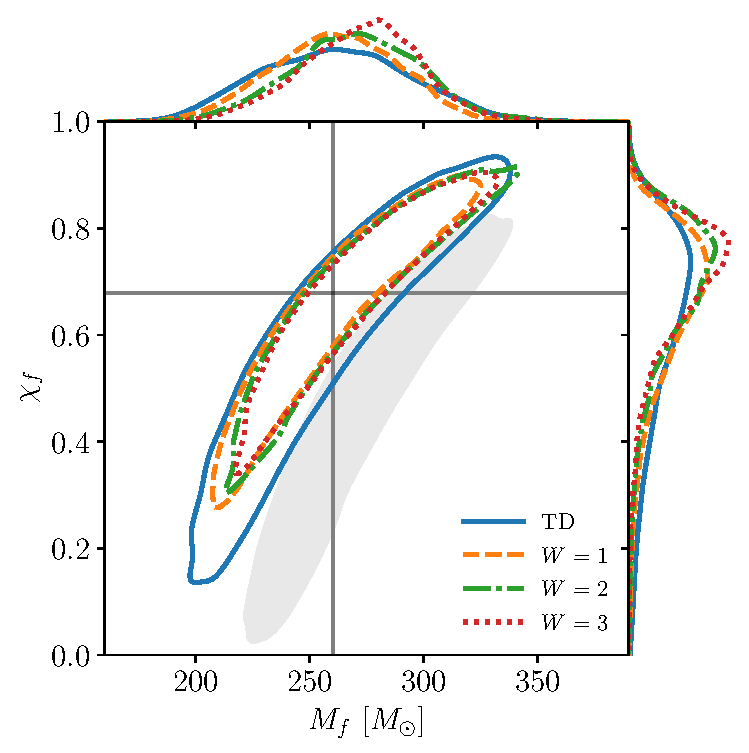
\includegraphics[width=0.6\columnwidth]{FrequencyDomainAnalysisofBlackHoleRingdowns/mass_spin_corner.pdf}
    \caption[Posteriors on the remnant mass and spin for a GW190521-like injection analysed while marginalising over the sky location and ringdown start time, for different numbers of wavelets]{ 
    Similar to Fig.~\ref{fig:mass_spin_corner_fixed_sky}, posteriors on the remnant mass and dimensionless spin for the GW190521-like injection using a single QNM while marginalising over the sky position, polarisation angle and ringdown start time.
    Also shown in the grey shaded region is the result of a frequency-domain analysis that does not include any wavelets (i.e.\ $W=0$); as expected, since this model has an abrupt discontinuity at $t_0$, this analysis yields severely biased estimates of the remnant mass and spin. 
    This $W=0$ analysis is included here to highlight the important role the wavelets play in our frequency-domain approach.
    }
    \label{fig:mass_spin_corner_zero_spin}
\end{figure}

\begin{figure}[t!]
    \centering
    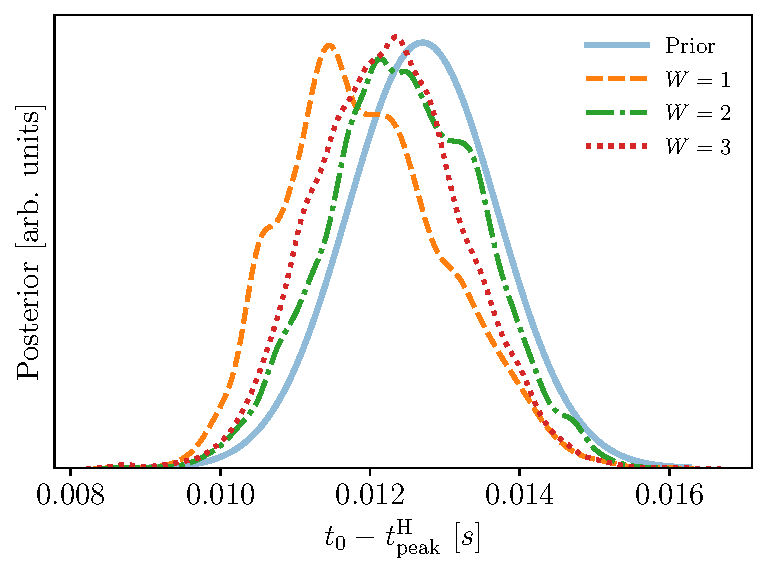
\includegraphics[width=0.6\columnwidth]{FrequencyDomainAnalysisofBlackHoleRingdowns/t0_prior_posterior.pdf}
    \caption[Posteriors on the ringdown start time for the same analyses as in Fig.~\ref{fig:mass_spin_corner_zero_spin}]{ 
    The prior and posterior distributions on the ringdown start time in the Hanford frame for the same frequency-domain analyses as in Fig.~\ref{fig:mass_spin_corner_zero_spin}. 
    The prior (solid blue line) is a Gaussian centred $12.7\,\mathrm{ms}$ after the time of peak strain in Hanford, with a standard deviation of $1\,\mathrm{ms}$. 
    This prior has been chosen to be informative; the posterior distributions do not differ significantly from the prior.
    It is necessary to use such an informative prior because we find that the ringdown start time cannot be reliably inferred solely from the data (see discussion in Section~\ref{subsec:t0}).
    We observe a slight preference for an early start time when using a small number of wavelets; we speculate that this is due to the wavelet model being less flexible than the maximally flexible model described in Section~\ref{subsec:motivation}.
    }
    \label{fig:t0_prior_posterior}
\end{figure}

We now turn to the case where the source sky position, polarisation angle and the ringdown start time are treated as free parameters in the frequency-domain analysis.
We use a uniform prior over the sphere of the sky and a flat, periodic prior on $\psi$ between $0$ and $\pi$.
As the sky position is now allowed to vary in the analysis, the time delay between the different interferometers and the geocenter is not constant. 
Therefore, for the ringdown start time, we choose to place a Gaussian prior on the start time in one of the detectors where the ringdown is clearly visible (we choose Hanford). 
The Gaussian prior was centred on the fixed value used in the time-domain analysis and has a relatively narrow width of $1\,\mathrm{ms}$ ($\sim 0.8\,M_f$).
This choice of prior is quite restrictive (i.e.\ assuming good prior knowledge of $t_0$) and the reasons for this are discussed further in Section~\ref{subsec:t0}; although, we note here that this is still more flexible than the delta-function prior used above.
The resultant posteriors on the remnant parameters are shown in Fig.~\ref{fig:mass_spin_corner_zero_spin}, and we see that the performance of our frequency-domain approach is not significantly degraded when the searching over $\alpha$, $\delta$, $\psi$ and $t_0$.
Shown in Fig.~\ref{fig:t0_prior_posterior} are the posteriors on the ringdown start time, $t_0$ which are discussed in more detail in the next section.

Stochastic sampling was performed using the \textsc{dynesty}~\cite{Speagle:2019ivv} implementation of the nested sampling algorithm~\cite{doi:10.1063/1.1835238, Skilling:2006gxv}.
For the sampling method, we used random walks with fixed proposals.
Typically, the minimum number of steps used in the random walk was 2000, and the number of live points was 4000.
We note that our frequency-domain ringdown analysis has many more parameters than a time-domain analysis due to the $5W$ parameters used in the wavelet sum.
Posteriors on these inspiral-merger parameters are not presented here, but we note that as the number of wavelets is increased strong degeneracies develop among these parameters.
This is expected, and is desirable in this context, as the wavelet part of the model is designed to be extremely flexible. 
These degeneracies in the inspiral-merger part of the model are not a problem for our present purpose as they do not inhibit our ability to measure the QNMs or the remnant properties. 
All posterior samples, including those for the wavelet parameters, are available at Ref.~\cite{finch_eliot_2021_5569759}.


\subsection{Determining the ringdown start time}\label{subsec:t0}

The ringdown start time, $t_0$, appears as a model parameter in our frequency-domain approach.
This raises two interesting questions: what prior should be placed on $t_0$, and how well can $t_0$ be measured from the data?
The possibility of determining $t_0$ from the data is particularly enticing because the ringdown start time is theoretically uncertain and its choice is crucial for any ringdown analysis.

\begin{figure}[t!]
    \centering
    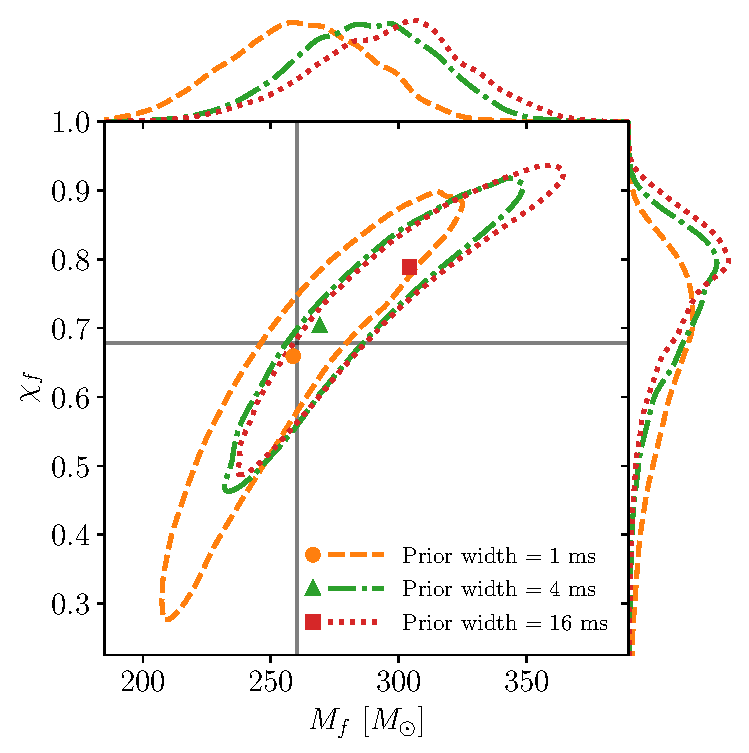
\includegraphics[width=0.6\columnwidth]{FrequencyDomainAnalysisofBlackHoleRingdowns/mass_spin_corner_widths.pdf}
    \caption[Posteriors on the remnant mass and spin for a GW190521-like injection, for different choices of ringdown start-time prior]{ 
    Similar to Fig.~\ref{fig:mass_spin_corner_zero_spin}, posteriors on the remnant mass and spin for the GW190521-like injection using a single wavelet ($W=1$) and a single QNM, but using different priors on $t_0$.
    The markers indicate the maximum likelihood values.
    The dashed orange curve is identical to that in Fig.~\ref{fig:mass_spin_corner_zero_spin}.
    }
    \label{fig:start_time_prior}
\end{figure}

\begin{figure}[t!]
    \centering
    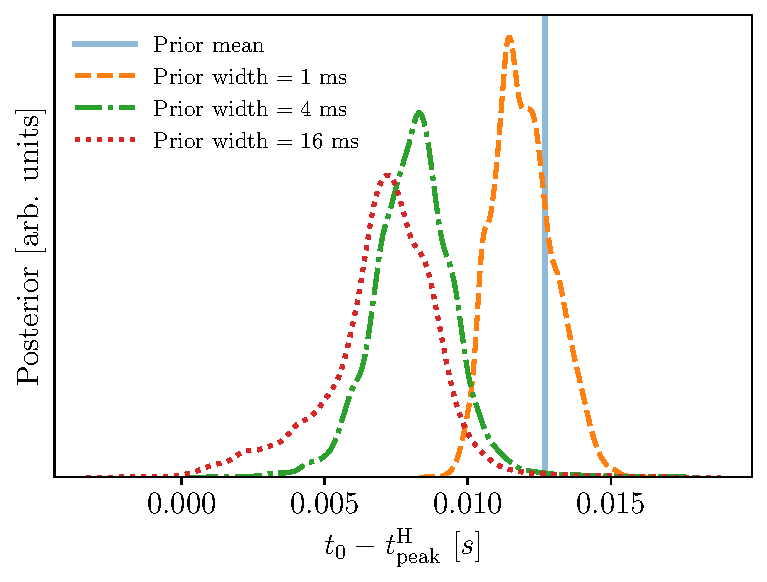
\includegraphics[width=0.6\columnwidth]{FrequencyDomainAnalysisofBlackHoleRingdowns/t0_prior_posterior_widths.pdf}
    \caption[Posteriors on the ringdown start time for the same analyses as in Fig.~\ref{fig:start_time_prior}]{ 
    Posteriors on the ringdown start time corresponding to Fig.~\ref{fig:start_time_prior}. 
    For each, the prior is a Gaussian centred on the vertical line, with widths given in the legend.
    It can be seen that a wider prior causes earlier ringdown start times to be favoured (this is the case even when additional wavelets are included). 
    As a result of the earlier start time, a bias appears in the recovered remnant parameters and higher values of both $M_f$ and $\chi_f$ are favoured.
    }
    \label{fig:start_time_posterior}
\end{figure}

Unfortunately, we find that when using wide priors on $t_0$, early ringdown start times are generally favoured and this leads to a bias in the recovered remnant mass and spin.
This can be seen in the results in Fig.~\ref{fig:start_time_prior}, where the $W=1$ analysis previously shown in Fig.~\ref{fig:mass_spin_corner_zero_spin} is repeated with increased values of the $t_0$ prior width.
The posterior on $t_0$ is also affected by the number of wavelets used;
as can be seen from the Fig.~\ref{fig:start_time_posterior}, larger values of $W$ tend to favour later ringdown start times. 
We have repeated the analyses in Fig.~\ref{fig:start_time_prior} with larger values of $W$ to see if this counteracts the preference for an early start time (and hence removes biases in the remnant parameters), however, this was found not to be the case.
These calculations show that the posterior obtained on the parameter $t_0$ in our approach depends on the prior and on the number of wavelets used in the (unphysical) model of the inspiral-merger signal.
Therefore, it does not seem to be possible to reliably measure the ringdown start time from the data alone.
It is for this reason that a narrow, informative, $t_0$ prior must be used in the analyses described in the previous section.
Although not desirable, this is still an improvement over the fixed $t_0$ routinely used in most time-domain analyses.

\begin{figure}[t!]
    \centering
    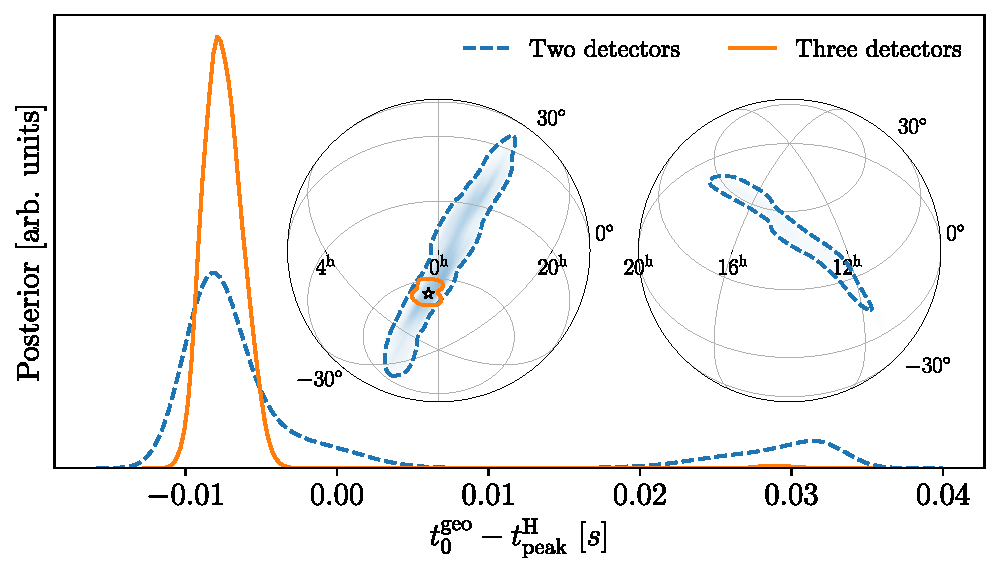
\includegraphics[width=0.9\columnwidth]{FrequencyDomainAnalysisofBlackHoleRingdowns/t0_geocent_posterior.pdf}
    \caption[Posteriors on the ringdown start time in the geocentric frame for a GW190521-like injection, for two- and three- detector networks]{ 
    \emph{Main panel:} posterior on the ringdown start time in the geocentric frame. The orange line corresponds to the $W=1$ model applied to the three-detector network injection (this is the same analysis presented in Figs.~\ref{fig:mass_spin_corner_zero_spin} and \ref{fig:start_time_prior}, which was plotted with a dashed orange line). 
    The dashed blue line corresponds to a similar analysis on a two-detector network injection (with Virgo removed). This is to motivate the choice to parameterise $t_0$ in the frame of a detector; in the geocentric frame, a multimodal structure appears as a result of different possible sky locations. This makes it harder to place a sensible prior.
    \emph{Left inset plot:} the sky location posterior on the southern hemisphere (orthographic projection). This contains the injected source location (indicated by the star) which is correctly recovered with sky area $\sim 77\ \mathrm{deg}^2$ (90\% confidence) for the three-detector network, and $\sim 1800\ \mathrm{deg}^2$ for the two-detector network.
    \emph{Right inset plot:} the northern hemisphere of the sky contains a secondary mode when using the two-detector network, which correlates with $t_0^\mathrm{geo}$. Both modes of the sky posterior are elongated along the circle of constant time delay between the two detectors.
    }
    \label{fig:t0_geocent_posterior}
\end{figure}

Finally, we discuss the choice that was made in the previous section to place the prior on $t_0$ in the frame of one of the interferometers.
Because the sky position is allowed to vary, using the geocenter time is inappropriate due to coupling with the sky position.
The orange curve in Fig.~\ref{fig:t0_geocent_posterior} shows the posterior on $t_0$ transformed into the geocenter frame from the $W=1$ frequency-domain analysis using the narrow $1\,\mathrm{ms}$ prior on the ringdown start time. 
Also shown in the blue-dashed line is a posterior from an identical injection into a two-interferometer H-L network.
Due to the multimodal sky posterior, the posterior on $t_0$ in the geocenter frame can also be multimodal (this is present in the three-detector analysis to a smaller extent but is most clear in the two-detector analysis).
This makes choosing a suitable prior for the ringdown start time more difficult in the geocenter frame.
It is for this reason that for the analyses described above, the prior was specified in the frame of one of the detectors.
The results in Fig.~\ref{fig:t0_geocent_posterior} also show that our frequency-domain approach yields a posterior on the source sky position as a by-product of the ringdown analysis. However, it should be stressed that this is not a ringdown-only result; the entire IMR model, including the unphysical wavelet part, is contributing to this sky localisation.


\subsection{Detecting additional QNMs}\label{subsec:overtones}

A key goal in the analysis of BH ringdowns is the detection of additional QNMs beyond the fundamental $\ell=m=2$, $n=0$ mode.
This has already been achieved; see, for example, Ref.~\cite{Isi:2019aib} where the $\ell=m=2$, $n=1$ overtone was identified in GW150914 using a time-domain analysis.
In this section we show, using our GW190521-like injection, that our frequency-domain approach is also able to identify additional QNMs.

\begin{figure}
    \centering
    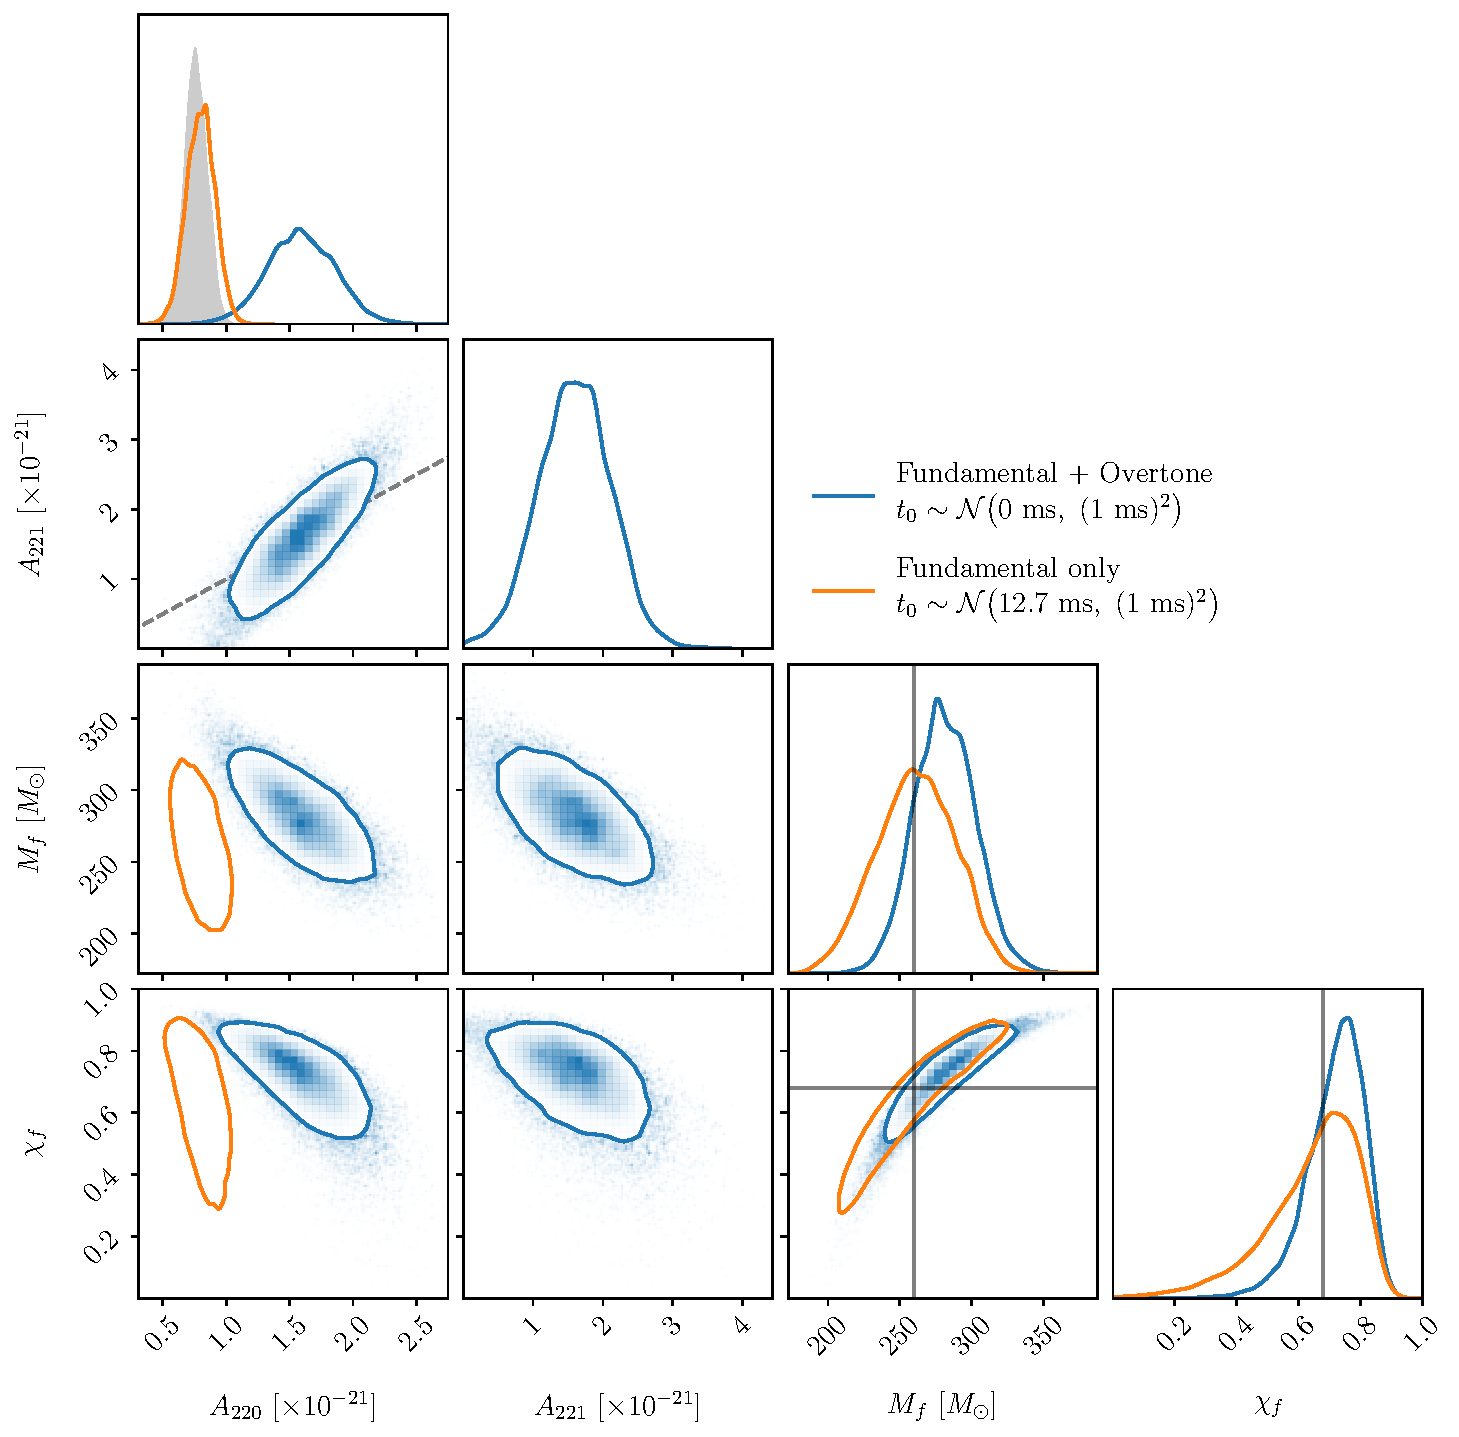
\includegraphics[width=0.9\columnwidth]{FrequencyDomainAnalysisofBlackHoleRingdowns/overtone_corner.pdf}
    \caption[Posteriors on the remnant mass and spin and on the quasinormal-mode amplitudes for a GW190521-like injection, for analyses with and without an overtone]{ 
    Posteriors on the QNM amplitudes and remnant mass and spin for one- and two-mode analyses (1QNM and 2QNM respectively) of the GW190521-like injection, performed in the frequency domain.
    The results in blue are for the recovery using two QNMs [the fundamental $(\ell,m,n)=(2,2,0)$ and its first overtone $(2,2,1)$] which are both detected with non-zero amplitudes using a $t_0$ prior centred on the time of the peak strain and with a width of $1\,\mathrm{ms}$.
    %
    Also shown in orange for comparison are the results using one QNM [the fundamental $(2,2,0)$ only] with a prior centred $12.7\,\mathrm{ms}$ after the peak, again with a width of $1\,\mathrm{ms}$.
    %
    The vertical and horizontal solid grey lines indicate the true values of the remnant mass and spin and the diagonal dashed grey line indicates $A_{220}=A_{221}$.
    %
    The difference in the $A_{220}$ amplitude between the two analyses can be explained by the different ringdown start times and the decay of the $(2,2,0)$ QNM.
    Over a time $\sim 12.7$ ms, we expect the $A_{220}$ amplitude to decay by a factor $\sim \exp[-12.7\,\mathrm{ms}/\tau_{220}] \sim 0.5$; this is shown in the shaded grey posterior in the top-left panel where the 2QNM posterior is used to predict the value of the amplitude at the later start time.
    % This is shown in the shaded grey posterior in the top-left panel where the results of the 2QNM analysis are used to predict the value of the amplitude at the later start time used by the 1QNM analysis.
    }
    \label{fig:overtone_corner}
\end{figure}

As a first step towards testing our model we search for the $n=1$ overtone of the fundamental QNM.
It would also be possible to search for higher harmonics (e.g.\ modes with $\ell\geq 3$); however, the results of previous investigations on NR simulations (see, e.g.\ Refs.~\cite{Giesler:2019uxc, Ota:2019bzl, Dhani:2020nik, Finch:2021iip}) suggest that overtones are generally more prominent than harmonics in the ringdown and are therefore a natural first target for any search.

We reanalyze the GW190521-like injection in the frequency domain using the $W=1$ inspiral-merger model but this time including an overtone in the ringdown (the choice to use a single wavelet is motivated by the previous results; it is sufficient to model the inspiral-merger for this high-mass injection, and we see no significant improvements with additional wavelets).
When using overtones, it is appropriate to start the ringdown analysis at an earlier time. 
For the frequency-domain analyses a Gaussian prior with a standard deviation of $1\,\mathrm{ms}$ centred at the time of the peak strain was used (this is $12.7\,\mathrm{ms}$ earlier than was used above).
The results of this ``2QNM'' analysis are shown in Fig.~\ref{fig:overtone_corner}, along with the fundamental only ``1QNM'' analysis for comparison.
Posteriors are plotted for the QNM amplitudes and the remnant mass and spin parameters. 
We see that the overtone can be confidently detected with non-zero amplitude.
The 2QNM analysis yields more precise measurements of the remnant mass and spin due to a combination of the earlier ringdown start time (which gives a larger ringdown SNR) and the improved ringdown model.

We now turn our attention to the resolvability of this additional QNM as a function of the injected SNR and compare the sensitivities of the time- and frequency-domain approaches.
The GW190521-like source was re-injected at a series of lower SNRs: 12, 9, and 6 (in the Livingston detector).
A $W=1$ frequency-domain analysis was re-performed on this sequence of injections, along with a time-domain analysis for comparison. 
Following the use of an earlier ringdown start time in the frequency-domain analysis, for the time-domain analysis the ringdown start time was fixed to the peak of the strain.
The posteriors on the amplitude $A_{221}$ of the overtone are shown in Fig.~\ref{fig:A221_posterior}.
As the SNR is decreased, the overtone becomes increasingly difficult to detect and the posteriors become consistent with $A_{221}=0$.
This is the case for both the time- and frequency-domain analyses which give similar results.
This suggests the time- and frequency-domain approaches are equally sensitive to additional QNMs.

\begin{figure}[t]
    \centering
    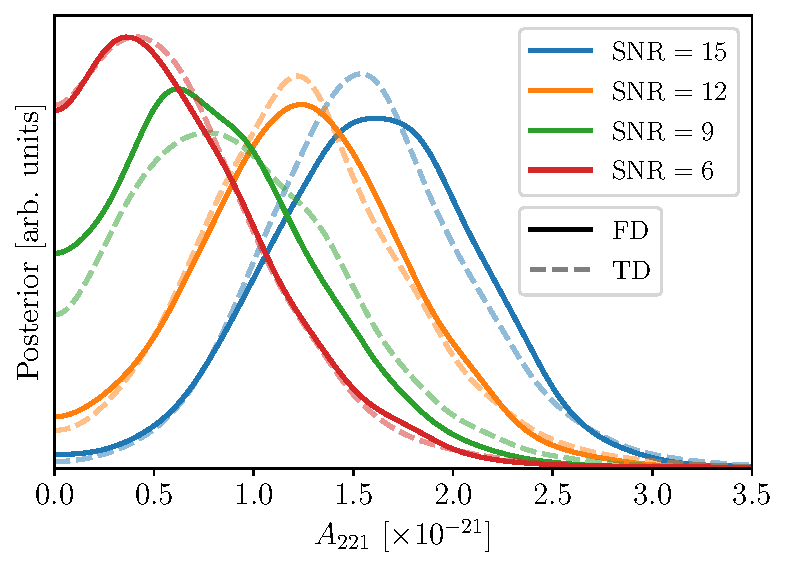
\includegraphics[width=0.6\columnwidth]{FrequencyDomainAnalysisofBlackHoleRingdowns/A221_posterior.pdf}
    \caption[Posteriors on the overtone amplitude for GW190521-like injections at a selection of signal-to-noise ratios, for both time- and frequency-domain analyses]{ 
    Overtone amplitude posteriors from a $W=1$ frequency-domain (FD) analysis, where the fundamental $(\ell,m,n) = (2,2,0)$ QNM and its first overtone $(2,2,1)$ are included in the ringdown model. 
    For comparison, the overtone amplitudes from a time-domain (TD) analysis are shown with the dashed lines. 
    The injected SNR in Livingston is controlled by changing the injection luminosity distance: $D_L = \{4016.3,\ 5020.4,\ 6693.9,\ 10040.8\}$ Mpc for $\mathrm{SNR} = \{15,\ 12,\ 9,\ 6\}$ respectively. 
    The maximum likelihood values scale as $D_L^{-1}$.
    }
    \label{fig:A221_posterior}
\end{figure}

Further evidence supporting this conclusion comes from the odds ratios (aka Bayes' factors) in favour of the overtone.
The Bayes' factors $\mathcal{B}^{2\mathrm{QNM}}_{1\mathrm{QNM}}$ (computed with equal prior odds) in favour of the second QNM were computed from both the time- and frequency-domain analyses. 
In order to do this, we perform an additional set of analyses on the series of injections used in Fig.~\ref{fig:A221_posterior} with the same ringdown start time (fixed at the peak for the time-domain analysis, and a Gaussian prior centred on the peak in Hanford for the frequency-domain) but without the overtone included.
We can then compute the evidence, $\mathcal{B}_{1\mathrm{QNM}}^{2\mathrm{QNM}}$, in favour of the 2QNM analysis (with an overtone) over the 1QNM analysis (fundamental mode only) keeping every other part of the analysis identical. 
The log-Bayes' factors for each of the different SNR injections are shown in Table.~\ref{tab:bayes_factors} where it can be seen that the time- and frequency-domain approaches are equally sensitive to the overtone mode.

\begin{table}[h!]
    \centering
    \begin{tabular}{c|cccc}
    SNR & 15   & 12   & 9   & 6  \\ \hline
    TD & $~ 1.1 ~$ & $0.3$ & $-0.3$ & $-0.7$ \\
    FD & $~ 1.1 ~$ & $~ 0.4 ~$ & $~ -0.4 ~ $ & $~ -0.6 ~$   
    \end{tabular}
    \caption[The log-Bayes' factors in favour of an overtone for the series of GW190521-like injections at different SNRs, for both time-domain and $W=1$ frequency-domain analyses]{ 
    The log-Bayes' factors $\log_{10}\mathcal{B}^{2\mathrm{QNM}}_{1\mathrm{QNM}}$ in favour of an overtone for the series of GW190521-like injections at different SNRs, for both time-domain (TD) and $W=1$ frequency-domain (FD) analyses. 
    The uncertainties on these Bayes' factors are all $\pm (0.1$ -- $0.2)$, with errors on the evidences estimated from within a single nested sampling run.
    }
    \label{tab:bayes_factors}
\end{table}


\section{GW150914-like injection}\label{app:GW150914}

In this chapter we test the frequency-domain approach further by analysing a GW150914-like injection, which will set up the analysis in the final chapter.

The surrogate was initialised with a total mass of $72.2\,M_\odot$ and a mass ratio of $1.16$. 
As before, all of the component spins were set to zero for simplicity. 
The simulated sky location and GW polarisation angle were taken to be $\alpha = 1.95$, $\delta = -1.27$, and $\psi = 0.82$. These are consistent with the GW150914 posterior and were chosen to match the values used in Ref.~\cite{Isi:2019aib}.
The distance to the binary was set to $471.4\,\mathrm{Mpc}$, which gave an optimal SNR in Hanford of 25.

The inclination angle was chosen to be $\pi$ (i.e\ the source is injected ``face-off'') which is consistent with the GW150914 posterior.
The source inclination affects the GW polarisation, and this is handled via the introduction of a ``ellipticity parameter'' $\epsilon$ which has the effect of transforming $h_\times(t) \rightarrow \epsilon h_\times(t)$.
For the ``face-on'' injections in the main text $\epsilon=1$ was used, while for the ``face-off'' injections considered here $\epsilon=-1$.
A more general analysis would allow $\epsilon$ to vary as a free parameter, such as what was done in Ref.~\cite{Isi:2021iql}.

We perform zero-noise injections into the two-interferometer H-L LIGO network that was operating at the time of the first detection. 
We use the PSDs associated with the data surrounding GW150914 (available at Ref.~\cite{gwtc1psds}).
These different parameters (particularly the lower total mass) result in a signal with a longer inspiral.
This is an important test case for our model as there is a much larger fraction of the SNR in the inspiral-merger (compared to the GW190521-like injection) which has to be ``marginalised out'' in the analysis.

\begin{figure}[t!]
    \centering
    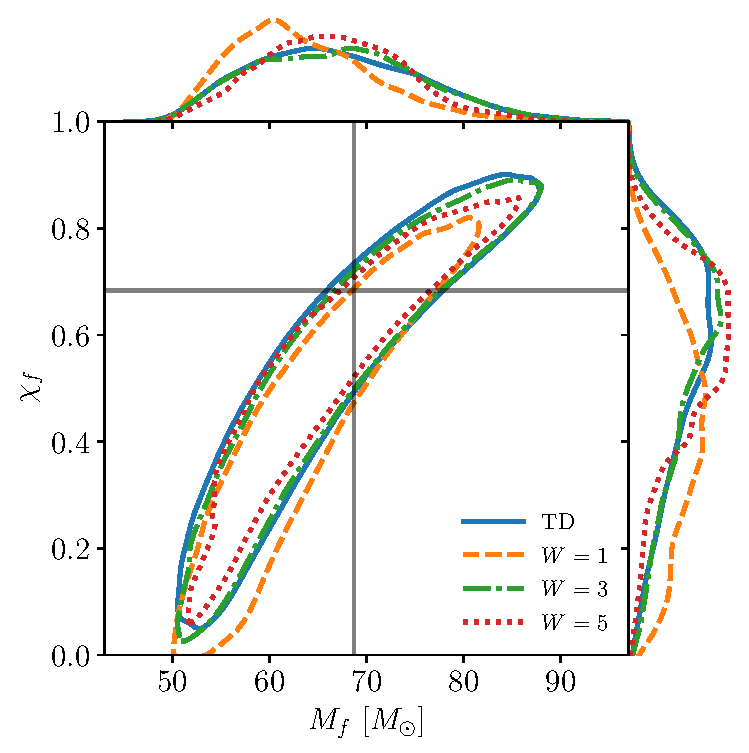
\includegraphics[width=0.6\columnwidth]{FrequencyDomainAnalysisofBlackHoleRingdowns/GW150914_mass_spin_corner.pdf}
    \caption[Posteriors on the remnant mass and spin for a GW150915-like injection]{ 
    Similar to Fig.~\ref{fig:mass_spin_corner_fixed_sky}, posteriors on the recovered remnant mass and spin for the GW150914-like injection using the fundamental QNM and a varying numbers of wavelets. 
    Also shown for comparison is the result of a time-domain analysis (solid blue line).
    }
    \label{fig:GW150914_mass_spin_corner}
\end{figure}

As was done initially for the GW190521-like injection, we fix the sky location and polarisation angle to the injected values to simplify the problem and aid comparison to the time-domain analysis.
The ringdown start time is also fixed to $3\,\mathrm{ms}$ after the time of the peak strain ($\sim 10\,M_f$ in geometric units).

Following the same procedure as in Section~\ref{sec:injection_study}, a time-domain analysis was first carried out to recover the fundamental QNM. 
The prior on the remnant mass was adjusted to reflect the lower injected value (flat between $50\,M_\odot$ and $100\,M_\odot$), but otherwise the analysis was unchanged from the time-domain analyses described in the main text.
The resultant remnant mass and spin posterior is shown by the blue solid line in Fig.~\ref{fig:GW150914_mass_spin_corner}.

Secondly, a series of frequency-domain analyses were carried out using an increasing number of wavelets.
Results for $W=1$, 3, and 5 are shown in Fig.~\ref{fig:GW150914_mass_spin_corner}.
We found a slightly more restrictive prior on the wavelet central times, $\eta_w$, was required to aid the inference; the Gaussian width was reduced to $10\,\mathrm{ms}$ ($\sim 30\,M_f$).
This encouraged the wavelets to fit near the ringdown start time, which is the part of the signal we are most interested in.
The upper bound on the wavelet frequencies was also increased to $500\,\mathrm{Hz}$ ($\sim 0.17\,M_f^{-1}$), as the lower binary mass means the merger-ringdown occurs at a higher frequency.
We see that a single wavelet is not quite sufficient to avoid bias in the remnant parameters, which may be expected when working with a longer inspiral.
As the number of wavelets is increased the bias disappears, and the remnant posteriors seem to converge to a solution that is stable against the inclusion of additional wavelets. 
As was the case for the GW190521-like analysis, we find the frequency-domain model achieves tighter constraints on the remnant parameters in comparison to the time-domain analysis. 

\begin{figure}[t!]
    \centering
    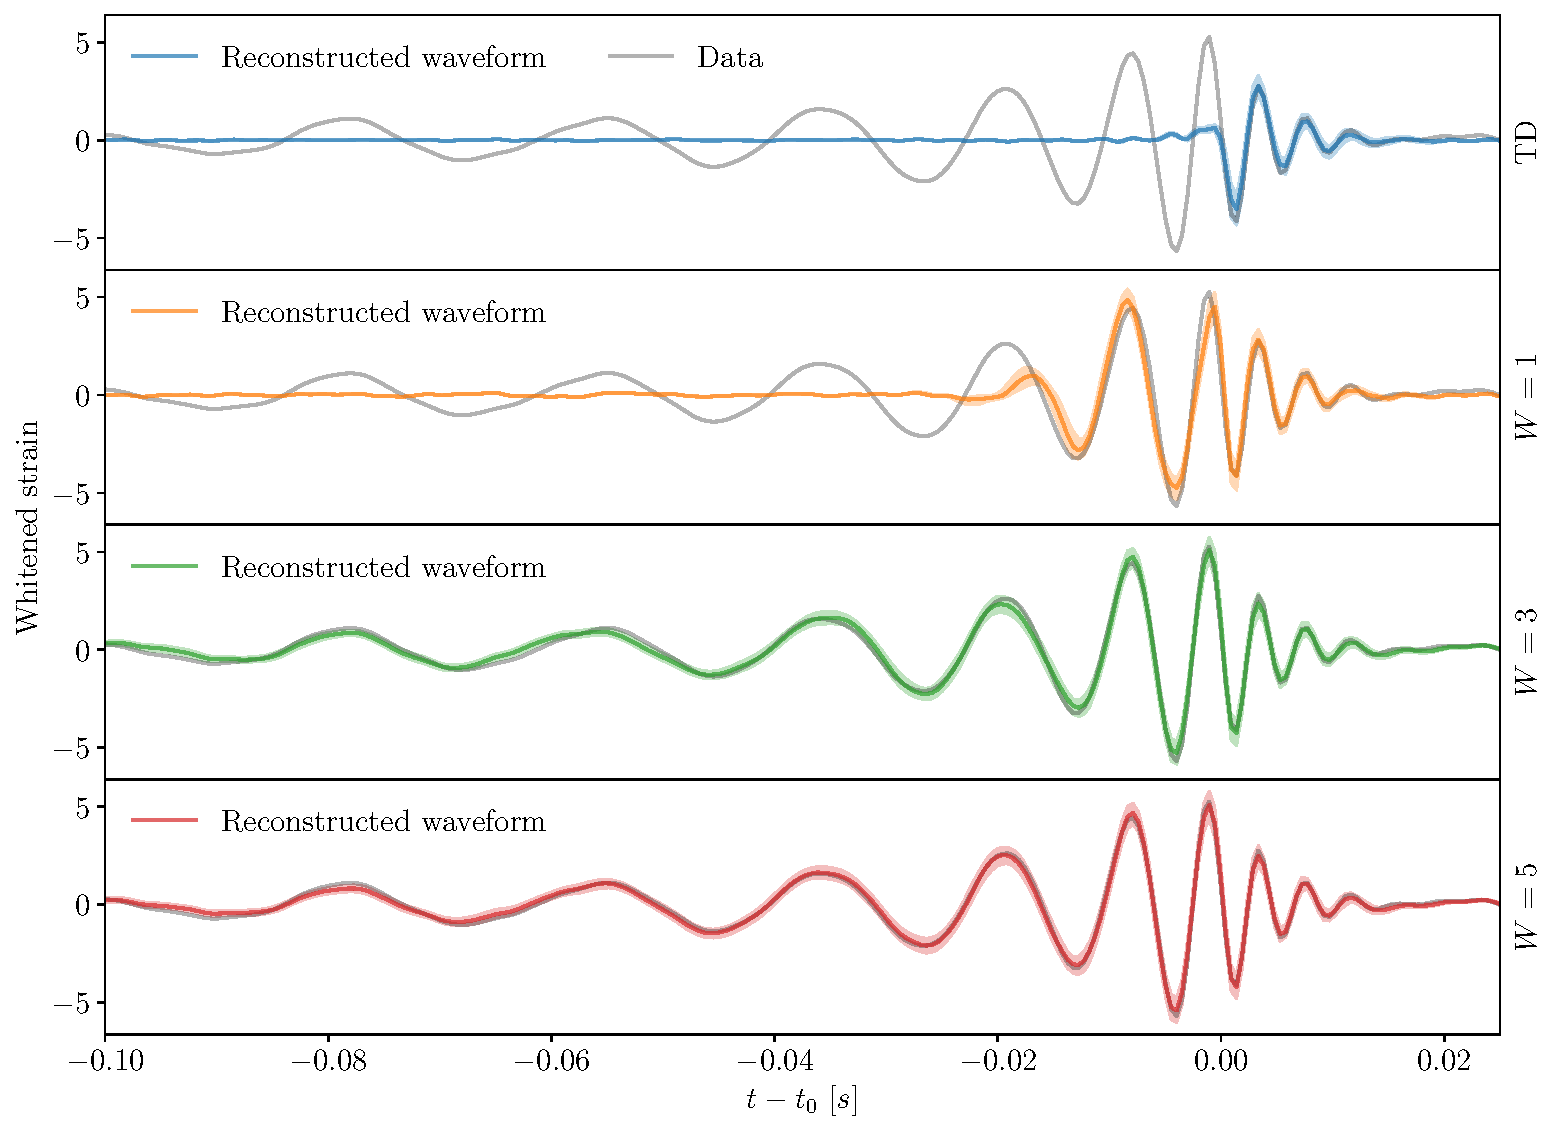
\includegraphics[width=0.9\columnwidth]{FrequencyDomainAnalysisofBlackHoleRingdowns/GW150914_whitened_waveforms.pdf}
    \caption[Whitened waveform reconstructions for the same analyses as in Fig.~\ref{fig:GW150914_mass_spin_corner}]{ 
    Whitened waveform reconstructions (in Hanford) corresponding to the results of Fig.~\ref{fig:GW150914_mass_spin_corner}. 
    The top panel shows the waveform from a time-domain analysis. 
    In the time-domain approach the data before the ringdown start time is excluded, but here the waveform is plotted for all times.
    This highlights one of the problems with using a ringdown-only model in the frequency domain: the abrupt start of the model leads to spectral leakage when Fourier transforming (visible as oscillations before the ringdown start time).
    The following panels show waveforms from the frequency-domain approach.
    Problems with spectral leakage are avoided, due to the wavelets smoothly connecting to the ringdown part of the model.
    Just a single wavelet fails to model the full GW150914-like inspiral-merger, which is to be expected because of its longer duration in-band.
    As more wavelets are included in the model, more of the inspiral-merger is captured by the model.
    The difference in the reconstruction for three and five wavelets is minimal, showing the model is converging on the signal.
    }
    \label{fig:GW150914_whitened_waveforms}
\end{figure}

Finally, we inspect the whitened waveform reconstructions for all four analyses shown in Fig.~\ref{fig:GW150914_mass_spin_corner}.
We focus on the waveform in the Hanford detector.
We take samples from the posterior of each run and use these to compute the projected waveform $F^\mathrm{H}_{+} h_+(t+\Delta t_\mathrm{H})+F^\mathrm{H}_{\times} h_\times(t+\Delta t_\mathrm{H})$, see Eq.~\ref{eq:projection_antenna}. This quantity is always discontinuous for both the time- and frequency-domain analyses.
We then whiten this waveform (and the data) using the Hanford PSD. After whitening, the projected waveform is continuous.
In Fig.~\ref{fig:GW150914_whitened_waveforms} we plot the median and $5\%-95\%$ credible region of the whitened waveform reconstructions.
The figure highlights the problem of spectral leakage, which occurs when taking Fourier transforms of discontinuous models. 
The time-domain model (top panel) has a discontinuity at the ringdown start time and this causes oscillations to appear before the start time in the whitened waveform.
The following panels, which include wavelets to model the inspiral-merger signal, remove this discontinuity and prevent Fourier transform artifacts.
A single wavelet is not sufficient to capture the full inspiral-merger signal, which likely causes the bias seen in Fig.~\ref{fig:GW150914_mass_spin_corner}. 
Increasing the number of wavelets makes the model flexible enough to model the inspiral-merger signal, and also to remove bias in the mass-spin posterior.



\section{Conclusions}\label{ch3:sec:discussion}

BH ringdown and QNMs are a key area of study in the burgeoning field of GW astronomy and are particularly important for testing GR.
Ringdown analyses are usually performed in the time domain as this provides a natural way to work with discontinuous models and to apply sharp cuts to the data. 
However, in these analyses the ringdown start time and sky position usually have been fixed beforehand.
The log-likelihood is also more computationally expensive than in the frequency domain.

We have presented a novel approach for analysing the ringdown in the frequency domain. 
Our approach uses a flexible combination of sine-Gaussian wavelets, truncated at the start of the ringdown, to effectively marginalise over the inspiral and merger parts of the signal. 
The benefits of performing the analysis in the frequency domain include being able to easily vary the source sky position and ringdown start time model parameters as part of the analysis.
As virtually all other GW data analysis is already performed in the frequency domain, a further benefit of our approach is that it allows us to utilise standard, and now very well-tested, GW analysis software packages for performing the Bayesian inference and also for estimating the noise properties.

We have tested our frequency-domain approach by analysing a series of NR surrogate injections and by comparing our results with those from a time-domain analysis. 
We find that our frequency-domain approach is equally sensitive to additional QNMs compared to the time-domain approach.
However, we find that it generally yields more precise measurements of the remnant BH mass and spin parameters which we speculate is due to some small coupling with the inspiral and merger signal.
We also paid particular attention to the choice of prior on $t_0$; although this appears as a model parameter in our approach it was found that, unfortunately, it was not possible to reliably determine it solely from the data.

In the next chapter we apply this method to real GW data.
Specifically the first GW event, GW150914, in a search for a ringdown overtone.

% Chapter 4

\chapter{Searching for a Ringdown Overtone in GW150914}

\label{Chapter4}

\section{Introduction}\label{ch4:sec:introduction}

The very first GW event, GW150914~\cite{LIGOScientific:2016aoc}, remains probably the best candidate for studying the ringdown.
This is a result of several factors, including its large SNR of $\rho\sim 24$ and its total mass of $M\sim 70\,M_\odot$ which places the merger and ringdown in the center of the LIGO~\cite{LIGOScientific:2014pky} sensitive frequency band at $\sim 200\,\mathrm{Hz}$. 
Additionally, GW150914 is by now the most well-studied GW event and therefore the signal and the properties of the noise in the surrounding data are extremely well understood.

The first tests of GR performed using GW150914 included an investigation of the ringdown~\cite{LIGOScientific:2016lio}. 
The ringdown signal, after a fixed starting time $t_0$, was modelled using a single damped sinusoid; the parameters of which were checked for consistency with the predicted least-damped QNM of the remnant BH.
This first attempt at a ringdown analysis was performed using the standard Whittle frequency-domain log-likelihood~\cite{10.2307/2983994}, commonly used in GW data analysis.
The ringdown was isolated by choosing a lower limit of $\sim 130\, \mathrm{Hz}$ in the frequency integral, effectively cutting the data mid-signal.
This approach suffers from several shortcomings. 
Firstly the frequency-domain cut at $\sim 130\, \mathrm{Hz}$ only approximately separates the ringdown from the early-time signal due to the breakdown of the stationary phase approximation near merger. 
Secondly the nonzero amplitude at the start of the signal model breaks the assumption of circularity for the Fourier transform, thereby introducing contamination in the form of spectral leakage. 
Therefore, this approach does not scale well to higher SNRs where noise will no longer dominate over the systematic errors introduced by the sharp frequency-domain cut.
Despite these drawbacks, this approach was successfully used in Ref.~\cite{LIGOScientific:2016lio} to identify the fundamental QNM in the GW150914 signal.

Since this initial attempt, several groups have developed new time-domain frameworks specifically for ringdown analyses~\cite{Carullo:2019flw, Isi:2019aib, Capano:2021etf}.
The principle motivation for working in the time domain is that it is easy to impose sharp cuts on the data at specific times (without any spectral leakage) and to analyse only data after a chosen start time (see Ref.~\cite{Isi:2021iql} for details of time-domain analysis methods).
These approaches have also enabled going beyond the fundamental mode. 
Generically, the ringdown can be modelled as a superposition of QNMs with complex frequencies $\omega_{\ell m n} = 2\pi f_{\ell m n} - i/\tau_{\ell m n}$, labelled with angular indices $\ell\geq 2$, $\abs{m}\leq\ell$, and an overtone index $n \geq 0$ [the fundamental mode has $(\ell, \abs{m}, n) = (2, 2, 0)$].
Detecting additional QNMs beyond the fundamental increases the scientific potential of ringdown studies, especially for fundamental tests of the Kerr metric, the no-hair theorems, and the BH area law~\cite{Dreyer:2003bv, Berti:2005ys, Gossan:2011ha, Brito:2018rfr, Carullo:2019flw, Isi:2019aib, Isi:2020tac}.

Outside of the testing-GR catalog papers mentioned previously~\cite{LIGOScientific:2020tif, LIGOScientific:2021sio}, other groups have attempted to identify additional QNMs in the ringdown data and perform tests of the no-hair theorem. 
This includes claims of detection of the $(2,2,1)$ overtone in GW150914~\cite{Isi:2019aib}, and claims of detection of the $(3,3,0)$ harmonic in GW190521~\cite{Capano:2021etf}. 
By allowing the QNM frequency of the secondary mode to deviate from the GR Kerr prediction, the above works found the measured spectrum to be in agreement with the no-hair hypothesis to within $\sim 20\%$ ($68\%$ credibility) and $\sim 1\%$ ($90\%$ credibility) respectively.

An early application of the time-domain framework was in Ref.~\cite{Isi:2019aib}, where Isi et al. claimed a detection of the first overtone of the fundamental QNM in the GW150914 signal [that is, the $(2, 2, 1)$ mode]. 
This was quickly followed by a separate detection claim of the $(3,3,0)$ harmonic mode in the signal of the $\sim 150M_\odot$ binary merger GW190521~\cite{LIGOScientific:2020iuh} by Capano et al.~\cite{Capano:2021etf} (this was done using an equivalent formulation of the time-domain method, although expressed in the frequency domain).
The claimed detection of an overtone was made possible partly because, compared to earlier studies, the authors chose to use an earlier start time for the ringdown; this was motivated by contemporary numerical relativity studies~\cite{Giesler:2019uxc} (see also Refs.~\cite{Bhagwat:2019dtm, Ota:2019bzl, Cook:2020otn, JimenezForteza:2020cve, Dhani:2020nik, Finch:2021iip, Forteza:2021wfq, Dhani:2021vac, MaganaZertuche:2021syq}) that demonstrated that when overtones are included the ringdown can be considered to start as early as the time of peak strain amplitude. 

However, a recent paper by Cotesta et al.~\cite{Cotesta:2022pci} reanalysed the GW150914 signal using very similar methods and found no significant evidence for an overtone.
It was also suggested that the earlier detection claims of Ref.~\cite{Isi:2019aib} were noise dominated.
(This prompted a response from Isi et al.~\cite{Isi:2022mhy} where they restated their claim to have detected an overtone in GW150914.) 
Ref.~\cite{Bustillo:2020buq} also found weaker evidence for an overtone using an analysis method closer to that of Ref.~\cite{LIGOScientific:2016lio}.
Similarly, the claim in Ref.~\cite{Capano:2021etf} that a harmonic had been detected in GW190521 has also been debated and no evidence for a harmonic was found by Ref.~\cite{LIGOScientific:2021sio}.
Amid this confusion, it is particularly concerning that the supposedly identical analyses in Refs.~\cite{Isi:2019aib, Isi:2022mhy}, and~\cite{Cotesta:2022pci} come to such different conclusions concerning which QNMs are in the data. 
Discrepancies of this sort risk jeopardising the science that can be done using future ringdown observations.

These discrepancies highlight some of the difficulties inherent in time-domain ringdown analysis, where important choices (that affect the results) for fixed quantities such as the ringdown start time have to be made and care must be taken with the noise covariance estimation.
If ringdown studies are to be used to make precision measurements of BH properties or as reliable tests of GR we must first be able to make reliable and reproducible determinations of the QNM content.
This is also not a problem that will be removed in the future with observations at higher SNR. Even if an event has a higher SNR that is sufficient for a clear detection of the first QNM overtone, the focus will then simply shift to trying to identify the next overtone (or else the next QNM harmonic) in the countably infinite ringdown sum~\cite{Bustillo:2020buq}.

To complement the time-domain analysis frameworks, in the last chapter we proposed a new method for ringdown analyses which works in the frequency domain.
A flexible sum of sine-Gaussian wavelets, truncated at the ringdown start time, is used to effectively marginalise over the inspiral-merger (i.e.\ pre-ringdown) part of the signal.
The model is completed by attaching this to the usual sum of QNMs which model the ringdown.
No continuity is enforced between the two parts of the model in order to keep the ringdown inference independent from the rest of the signal.
However, we find the continuity is effectively learned from the data, and any remaining discontinuities disappear entirely when the signal is ``whitened’’ according to the instrumental noise.
In a particular limit, this approach can be shown to be formally equivalent to the time-domain analyses described above.
However, this frequency-domain approach can be generalised and offers several advantages over time-domain approaches:
well-established GW data analysis methods and pipelines can be used (which are all built in the frequency domain), 
the inspiral-merger data informs the noise estimation at the start of the ringdown (improving parameter estimation accuracy), 
and the ringdown start time and the source sky position can be easily treated as free parameters and marginalised over as part of a Bayesian analysis (instead of being fixed).
We note, however, that (as discussed in Chapter~\ref{Chapter3}) a narrow and informative prior on the ringdown start time must be used.
Reweighting techniques can be employed to investigate different ringdown start time prior choices computationally efficiently in post processing (see Section~\ref{subsec:reweighting}) obviating the need for the large number of analyses performed in Refs.~\cite{Cotesta:2022pci, Isi:2022mhy}.

In this chapter the new frequency-domain method is applied to reanalysing the ringdown of GW150914 paying particular attention to the presence (or absence) of an overtone. 
We perform analyses with and without an overtone and investigate different choices of the ringdown start time. 
We also perform additional analyses with varying data sampling frequencies and integration limits to verify the stability of our results. Finally, a mock injection study into real detector noise is also performed to further assess the significance of any overtone detection.
Section~\ref{sec:analysis} describes the signal model, the data, and the analysis methods used in this chapter.
Section~\ref{sec:results} presents our main results including posteriors on the remnant BH properties and overtone amplitude, and Bayes' factors for the overtone model.
The results are discussed further in Section~\ref{ch4:sec:discussion}.
Throughout this chapter we make use of natural units where $G=c=1$.

All data products and plotting scripts used to make the figures in this chapter are made publicly available at Ref.~\cite{finch_eliot_2022_6949492}.


\section{Methods}\label{sec:analysis}

This section briefly describes the frequency-domain method for analysing BH ringdowns introduced in Chapter~\ref{Chapter3}:
the wavelet-ringdown model is described in Section~\ref{sec:model}; the data, likelihood and priors are described in Section~\ref{sec:details}; and our approach for dealing with changes to the ringdown start time is described in Section~\ref{subsec:reweighting}.


\subsection{Wavelet-ringdown model}\label{sec:model}

Our model consists of two parts: one for early times before $t_0$ which is referred to here as the \emph{inspiral-merger}, and another for the \emph{ringdown} after the start time $t_0$.

First, we describe the ringdown part of the model.
After a ringdown start time $t_0$, which is itself a parameter in the model, the model takes the form
\begin{equation}\label{eq:ringdown_model}
    h^\mathrm{R}(t) = h_+^\mathrm{R}(t) + ih_\times^\mathrm{R}(t) = \sum_{n=0}^N A_n e^{-i[\omega_{22n}(t-t_0) + \phi_{n}]}, \quad t \geq t_0. 
\end{equation}
Because our focus in this chapter is on the presence of an overtone, we fix the angular indices to $\ell = m = 2$ and vary only the number of QNM overtones, $N$, in the model ($N$ is always taken to be either 0 or 1 in this chapter). 
Note that the form of this equation differs slightly from Eq.\ref{ch3:eq:hr} in Chapter~\ref{Chapter3}. 
This is because the source inclination angle is fixed to be ``face-off'' (i.e.\ $\iota=\pi$).
In the notation of (for example) Refs.~\cite{Dhani:2020nik, Finch:2021iip, MaganaZertuche:2021syq}, this is equivalent to using the $\ell = -m = 2$ mirror modes. 
Or, in notation of Ref.~\cite{Isi:2021iql}, using an ellipticity of $\epsilon = -1$.
The complex QNM frequencies, $\omega_{\ell m n} = 2\pi f_{\ell m n} - i/\tau_{\ell m n}$, are functions of the remnant BH mass $M_f$ (detector frame) and dimensionless spin $\chi_f$.
Additionally, each QNM is further described by an amplitude, $A_{n}$, and a phase, $\phi_{n}$. 

Second, we describe the inspiral-merger part of the model.
This is modelled as a truncated sum of $W$ wavelets.
At early times the model takes the form
\begin{align}\label{eq:wavelets}
	h^\mathrm{IM}(t) &=  h_+^\mathrm{IM}(t) + ih_\times^\mathrm{IM}(t) \nonumber \\
	&= \sum_{w=1}^{W} \mathcal{A}_w \exp \Bigg[-2\pi i \nu_w(t-\eta_w) - \qty(\frac{t-\eta_w}{\tau_w})^2 - i\varphi_w \Bigg], \quad t < t_0. 
\end{align}
Again, the minor differences in sign conventions compared to Chapter~\ref{Chapter3} come from fixing the inclination angle to be face-off. 
The wavelets are each described by five parameters: $\mathcal{A}_w$ and $\varphi_w$ are the wavelet amplitudes and phases, $\tau_w$ are the wavelet widths, $\nu_w$ are the wavelet frequencies, and $\eta_w$ are the wavelet central times. 
In this chapter we use $W=3$ (three wavelets) in our model.
This number was empirically found to be sufficient (see Section~\ref{app:GW150914}, where the number of wavelets was varied for a GW150914-like injection).

The full signal model is given by discontinuously joining the inspiral-merger to the ringdown at $t_0$,
\begin{equation}
	h(t) = h^\mathrm{IM}(t) + h^\mathrm{R}(t).
\end{equation}

Finally, the detector response must be considered.
We project the waveform polarisations onto each interferometer (IFO) with the antenna patterns, $F^\mathrm{IFO}_{+,\times}$.
The detector response for each ${\mathrm{IFO}\in \{\mathrm{H}, \mathrm{L}\}}$ is given by
\begin{align} \label{ch4:eq:projection_antenna}
	h^\mathrm{IFO}(t) = F^\mathrm{IFO}_+(\alpha, \delta, \psi) ~ &h_+(t + \Delta t_\mathrm{IFO}) \nonumber \\
	+ F^\mathrm{IFO}_\times(\alpha, \delta, \psi) ~ &h_\times(t + \Delta t_\mathrm{IFO}),
\end{align}
where $\alpha$, $\delta$ are the source right ascension and declination, and $\psi$ is the GW polarisation angle.
The time delay $\Delta t_\mathrm{IFO}(\alpha, \delta)$ accounts for the different signal arrival times at the detectors and is also a function of the source sky location.
Throughout this chapter we quote times in the Hanford frame.
So, in particular, $t_0$ refers to the ringdown start time in Hanford.
By definition, $h_+(t) = \Re\{ h(t) \}$, and $h_\times(t) = \Im \{ h(t) \}$.


\subsection{Data and priors}
\label{sec:details}

We use the GW150914 strain data sampled at $4096\, \mathrm{Hz}$ for both the Hanford and Livingston interferometers, which was obtained from Refs.~\cite{gwosc, LIGOScientific:2019lzm}.
A total of $4096\,\mathrm{s}$ of data around the event was downloaded, from which the mean was subtracted (this is effectively equivalent to applying a $\sim 1\, \mathrm{Hz}$ highpass filter). 
Pre-computed power spectral densities (PSDs) associated with GW150914 from the GWTC-1 release were used~\cite{gwtc1psds}. 
It has been verified our results are insensitive to the exact noise PSD used; for example, our results are unchanged when using a PSD estimated from a length of off-source data.
The analysis data consists of $4\,\mathrm{s}$ of data centred on the event GPS time ($1126259462.4\,\mathrm{s}$), and a Tukey window with an alpha parameter of 0.2 was applied to this analysis data.
The Bayesian analysis used the standard frequency-domain log-likelihood function (see, e.g., Eq.~\ref{eq:logL_FD_continuous}), with the limits of the frequency integration between $20$ and $1000\, \mathrm{Hz}$.
The choices of sampling rate and upper limit of frequency integration are discussed further in Section~\ref{subsec:noise}.

All the model parameters described in Section~\ref{sec:analysis} were sampled over as part of a Bayesian analysis.
For the wavelet parameters, uniform priors are used for the amplitudes $(\mathcal{A}_w \in [0,10^{-20}])$, phases $(\varphi_w \in [0,2\pi])$, frequencies $(\nu_w \in [20,200]\, \mathrm{Hz})$, and widths $(\tau_w \in [4,80]\, \tilde{M_f}$, or equivalently $\sim[1.4,27]\, \mathrm{ms})$.
Here, $\tilde{M_f}=68.779M_\odot=0.33875\,\mathrm{ms}$ is a fixed point estimate of the final, detector-frame mass (obtained using the median value from Ref.~\cite{LIGOScientific:2018mvr}) and should not be confused with the varying model parameter $M_f$.
The label-switching ambiguity among the wavelets was removed by enforcing the ordering 
$ \nu_w \leq \nu_{w+1} $ via the hypertriangulation transformation described in Ref.~\cite{Buscicchio:2019rir}.
We sample over the wavelet central times ($\eta_w$) using a Gaussian prior in the Hanford frame with a width of $50\,\tilde{M_f}$ ($\sim 17\,\mathrm{ms}$) centred on $t_\mathrm{ref} = 1126259462.423\,\mathrm{s}$.
This choice was found to be sufficiently flexible, whilst at the same time encouraging the wavelets to accurately model the signal near the peak (see the discussion in Section~\ref{app:GW150914}).

For the ringdown, uniform priors are used for the amplitudes $(A_n \in [0,10^{-19}])$, phases $(\phi_n \in [0,2\pi])$, remnant mass $(M_f \in [40,100]\,M_\odot )$, remnant spin $(\chi_f \in [0,0.99])$ and ringdown start time $(t_0-t_\mathrm{ref} \in [-15, 15]\,\tilde{M_f},$ which in SI units corresponds to $\sim[-5.1,5.1]\, \mathrm{ms})$.
We use a uniform prior on $t_0$ so that the samples can be easily reweighted in post-processing (see Section~\ref{subsec:reweighting}). 
For the remaining parameters, we used a uniform prior over the sphere of the sky (parameterised using $\alpha$ and $\delta$) for the source location and a flat, periodic prior on the polarisation angle $\psi$ in the range $0$ to $\pi$.

The nested sampling~\cite{Skilling:2006gxv} algorithm as implemented in \textsc{dynesty}~\cite{Speagle:2019ivv} was used to sample the posterior with 4000 live points and using the random walk sampling method with a walk length parameter of 2000.


\subsection{Reweighting} \label{subsec:reweighting}

An ever present issue in ringdown analyses is the choice of ringdown start time, $t_0$, and this choice is closely related to the issue of the presence of an overtone.
To address this issue, previous time-domain analyses~\cite{Isi:2019aib, Cotesta:2022pci, Isi:2022mhy} perform large numbers of Bayesian analysis runs with different choices of start time.

One key conceptual benefit of the frequency-domain approach of Chapter~\ref{Chapter3} is that the ringdown start time enters as a parameter of the model and can therefore be easily marginalised over, instead of simply being fixed (although, see Ref.~\cite{Carullo:2019flw} where the ringdown start time was varied in a time-domain analysis). 
However, it is necessary to choose an informative (narrow) prior for the parameter $t_0$.

A related computational benefit of our approach is that we can do a single Bayesian analysis run with a broad uniform prior on $t_0$. 
We can then explore different, narrower priors by reweighting the results in post processing. 
This is an example of importance sampling (see, for example, Ref.~\cite{RobertChristian2013MCsm}) and is the approach adopted here.
This removes the need to perform the large number of runs used to explore the effect of varying the ringdown start time when performing time-domain ringdown analyses.

Given a model that depends on parameters $\params$, a likelihood $\mathcal{L}(\mathrm{data}|\params)$, and a prior $\pi(\params)$, nested sampling can be used to draw a large number of samples $\params_i$ from the posterior, which is given by Bayes' theorem $P(\params|\mathrm{data})\propto \mathcal{L}(\mathrm{data}|\params) \pi(\params)$.
Samples from the posterior have associated weights $w_i$ (samples may often be equally weighted with $w_i=1$, but we do not require this to be the case). 
Such samples can be used to approximate integrals via a Monte-Carlo sum; $\int \mathrm{d}\params\,P(\params|\mathrm{data})f(\params)=\sum_{i}w_i f(\params_i)/W$, where $W=\sum_{i}w_i$.
If we choose a new prior $\hat{\pi}(\params)$, then the Bayesian posterior is given instead by $\hat{P}(\params|\mathrm{data})\propto \mathcal{L}(\mathrm{data}|\params) \hat{\pi}(\params)$.
We can define the new weights via
\begin{align}
	\hat{w}_i = w_i \frac{\hat{\pi}(\params_i)}{\pi(\params_i)}.
\end{align}
The same samples can then be used to approximate integrals of the form $\int \mathrm{d}\params\,\hat{P}(\params|\mathrm{data})f(\params)$ via the Monte-Carlo sum $\sum_{i}\hat{w}_i f(\params_i)/\hat{W}$, where $\hat{W}=\sum_{i}\hat{w}_i$.

It is also possible to reweight the Bayesian evidence for the new choice of prior.
In a GW context this approach has been used previously for inference with higher-order modes~\cite{Payne:2019wmy}.
The Bayesian evidence (i.e.\ the normalisation denominator in Bayes' theorem) under the original prior is given by $Z=P(\mathrm{data})=\int\mathrm{d}\params\,\mathcal{L}(\mathrm{data}|\params)\pi(\params)$.
The Bayesian evidence under the new prior, $\hat{\pi}(\params)$, is $\hat{Z}=\int\mathrm{d}\params\,\mathcal{L}(\mathrm{data}|\params)\hat{\pi}(\params)$. Using the reweighted samples to approximate the integral, it can be shown that the new evidence is given by
\begin{align}\label{eq:new_evidence}
	\hat{Z} = Z\frac{\hat{W}}{W}.
\end{align}

\begin{figure}[t]
    \centering
    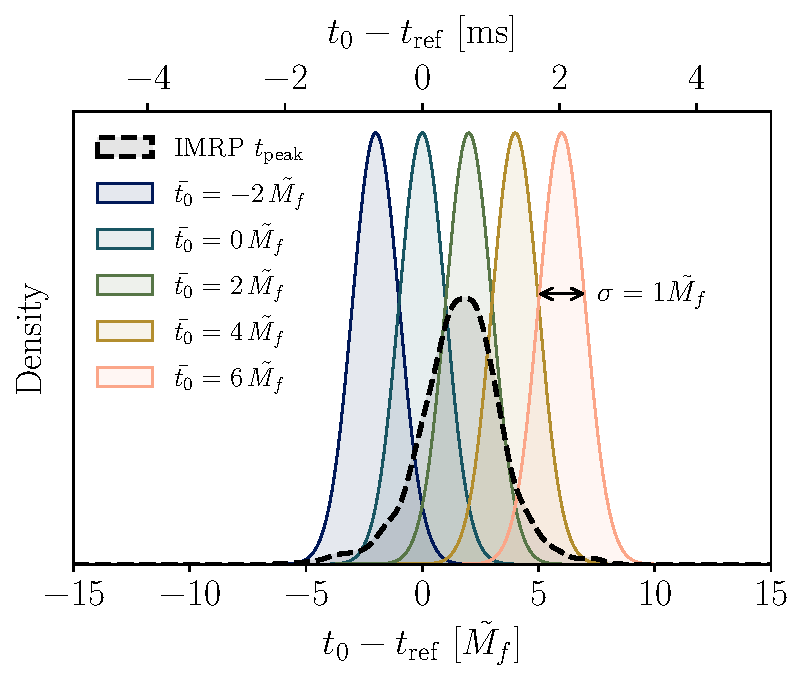
\includegraphics[width=0.6\columnwidth]{SearchingforaRingdownOvertoneinGW150914/start_time_plot.pdf}
    \caption[Different prior choices for the ringdown start time used for the GW150914 analysis]{ 
    Our ringdown inference is run initially using a flat, uniform prior on the ringdown start time, $t_0$, over the plot range $\pm 15 \tilde{M_f}$ relative to $t_\mathrm{ref}$ (Hanford frame).
    In post processing, the posterior samples can be reweighted to a different choice of prior on $t_0$ (see Section~\ref{subsec:reweighting}). 
    The different prior choices used in this chapter are shown in this figure. 
    We use a sequence of narrow Gaussian priors (with different means $\bar{t_0}$ defined relative to $t_\mathrm{ref}$ and fixed standard deviation, $\sigma=1\tilde{M_f}$) as well as using the posterior on the time of peak strain from a full IMR analysis as a prior.
    }
    \label{fig:start_time}
\end{figure}

The process of reweighting to the new, target prior reduces the effective number of posterior samples available.
For this not to be a problem, we require the original prior to have significant support across the target prior.
Here, we reweight on just a single parameter, the ringdown start time $t_0$.
As described above, we use a uniform prior on $t_0$ as the original prior, $\pi$, in our analyses.
For the target prior we use a variety of different choices, this removes the need for performing a large number of runs with different start times. 
Our prior choices are plotted in Fig.~\ref{fig:start_time}.
Narrow Gaussians centred at different start times are used to explore the start time dependence on the results, and we use the notation $\bar{t_0}$ to indicate the mean of the Gaussian relative to $t_\mathrm{ref}$. 
For more details on the $t_0$ reweighting, see Section~\ref{app:t0_posterior_prior}.

We also use the posterior on $t_\mathrm{peak}$ from a full inspiral-merger-ringdown (IMR) analysis from Ref.~\cite{Isi:2022mhy}, obtained with the \textsc{IMRPhenomPv2} (IMRP) waveform model~\cite{Hannam:2013oca}, as another prior on $t_0$. 
Our aim in doing this is to marginalise over our uncertainty on the ringdown start time, $t_0$. 
We emphasise that this is achieved here by using the posterior on the time of peak strain as a prior on $t_0$; this is motivated by the observations of Refs.~\cite{Giesler:2019uxc, Bhagwat:2019dtm, Ota:2019bzl, Cook:2020otn, JimenezForteza:2020cve, Dhani:2020nik, Finch:2021iip, Forteza:2021wfq, Dhani:2021vac, MaganaZertuche:2021syq} described above, which show that generically the ringdown can be considered to start at around this time.


\section{Results}\label{sec:results}

There are several ways to investigate and quantify the evidence for additional QNMs in the ringdown.
Section~\ref{subsec:overtone} contains the results of a series of analyses designed to study the presence of a possible overtone in GW150914.
Section~\ref{subsec:verify} contains the results of a series of analyses designed to test whether or not what has been detected really is an overtone and is not the accumulation of other effects.
Section~\ref{subsec:noise} describes further checks on the stability of the results, and Section~\ref{subsec:other_results} contains some additional results that further demonstrate the capabilities of the frequency-domain approach to ringdown analysis.

Throughout Secs.~\ref{subsec:overtone} and \ref{subsec:verify}, we compare our results with those in Refs.~\cite{Cotesta:2022pci} and~\cite{Isi:2022mhy}. 
This is done in the hope of helping to resolve the controversy over the evidence for a ringdown overtone in GW150914. 
However, it should be stressed that our results are produced using a very different method and care should therefore be taken in making direct comparisons.
Although the frequency-domain analysis is formally equivalent to the time-domain analysis in a particular limit (as discussed in the introduction, and in more detail in Section~\ref{subsec:motivation}) we do not take this limit in a practical analysis. Furthermore, the frequency-domain analysis is further generalised with respect to the time-domain analysis in that it marginalises over parameters such as the sky position and ringdown start time (which are fixed in the analyses of Refs.~\cite{Cotesta:2022pci, Isi:2022mhy}).
Results from our frequency-domain analyses should therefore not be expected to agree perfectly with those from previous time-domain analyses.

\subsection{Presence of an overtone}\label{subsec:overtone}

In order to investigate the presence of an overtone in the GW150914 ringdown, we initially perform two analyses using the model described in Section~\ref{sec:model}: one analysis uses only the fundamental QNM ($N=0$) and the other includes the first overtone ($N=1$).
Aside from the inclusion of the overtone in the ringdown (which introduces two additional parameters: an amplitude and a phase), these two analyses are otherwise identical.

\begin{figure}[t]
    \captionsetup[subfigure]{labelformat=empty}
    \centering
    \;\subfloat{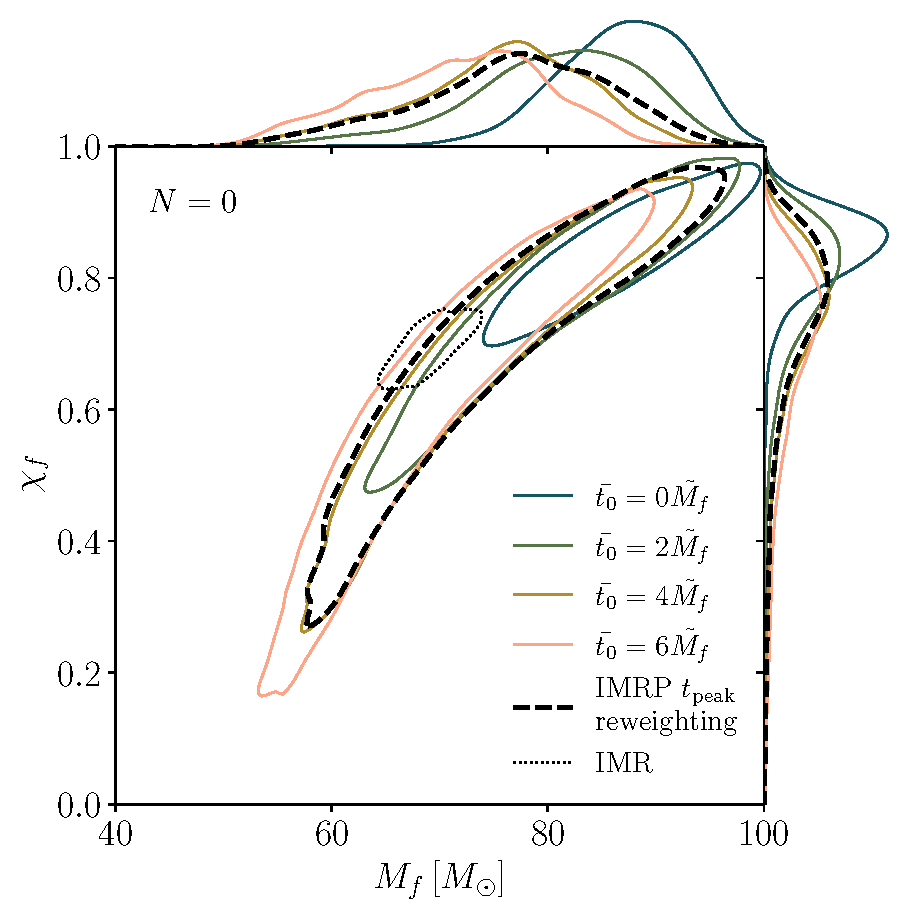
\includegraphics[width=.49\linewidth]{SearchingforaRingdownOvertoneinGW150914/220_mass_spin_plot.pdf}}
    \;\subfloat{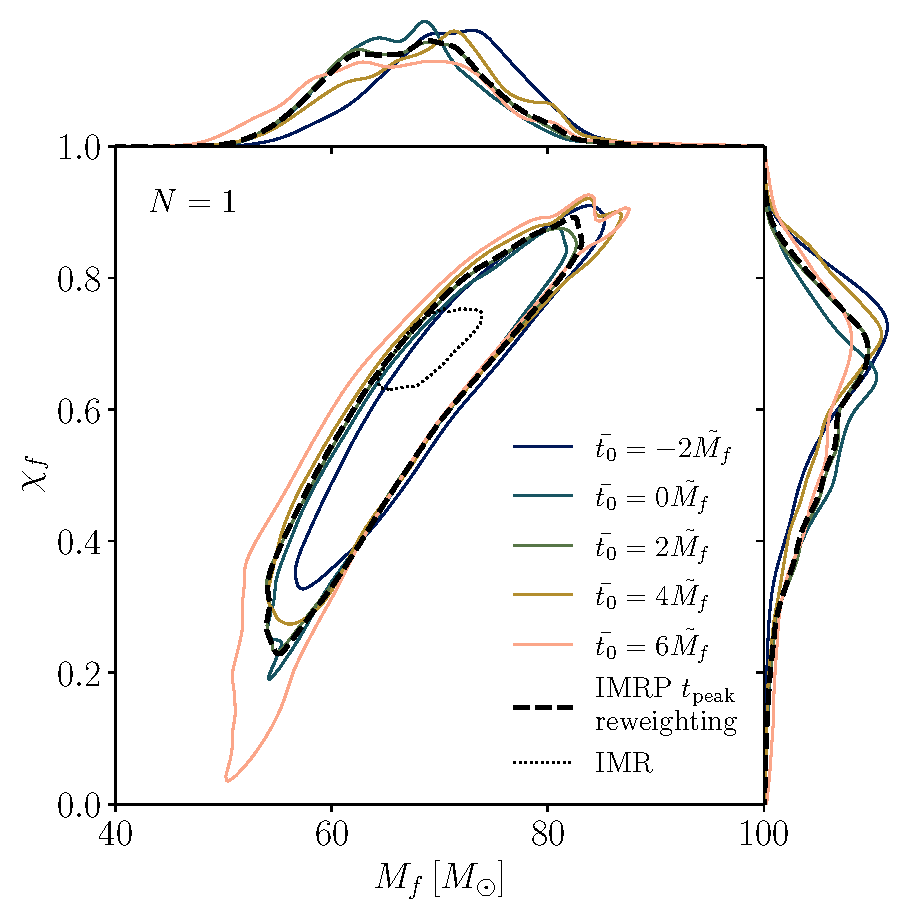
\includegraphics[width=.49\linewidth]{SearchingforaRingdownOvertoneinGW150914/220221_mass_spin_plot.pdf}}
    \caption[Posterior distributions on GW150914's remnant mass and dimensionless spin for different choices of $t_0$ prior]{  
    Posterior distributions on the remnant mass, $M_f$, and dimensionless spin, $\chi_f$, for different choices of $t_0$ prior (the colours and line styles correspond to those used in Fig.~\ref{fig:start_time}). 
    \emph{Left:} the results from the $(2,2,0)$ fundamental-mode-only analysis (i.e.\ $N=0$).
    \emph{Right:} the results from the overtone analysis including the $(2,2,0)$ and $(2,2,1)$ modes (i.e.\ $N=1$).
    Each line corresponds to a different choice of $t_0$ prior. 
    Coloured lines correspond to Gaussians with widths of $1 \tilde{M_f}$ and means $\bar{t_0}$ (see Fig.~\ref{fig:start_time}).
    The dashed black line corresponds to using the posterior on time of peak strain (from a full IMR analysis) as our prior, which marginalises over uncertainty on the time of peak strain.
    Also shown for reference (dotted line) is the posterior from a full IMR analysis. 
    The main panel shows the 90\% confidence contours while the side panels show the one-dimensional marginalised posteriors.
    }
    \label{fig:mass_spin_post}
\end{figure}

In Fig.~\ref{fig:mass_spin_post} we plot the posterior distributions on the remnant BH mass, $M_f$, and dimensionless spin, $\chi_f$, for both of these analyses.
Results are shown for the different choices of the prior on the ringdown start time shown in Fig.~\ref{fig:start_time} (these results were obtained by reweighting the samples obtained with a flat prior using the approach described in Section~\ref{subsec:reweighting}).
The earliest start time ($\bar{t_0}=-2\tilde{M_f}$) is omitted from the fundamental-only ($N=0$) plot in the left-hand panel of Fig.~\ref{fig:mass_spin_post} because of a low number of posterior samples at these time (see Section~\ref{app:t0_posterior_prior}).
Also shown for comparison are the much tighter constraints resulting from the full IMR analysis.
These IMR posterior samples were obtained from Ref.~\cite{maximiliano_isi_2022_5965773}, which (as detailed in Refs.~\cite{Isi:2019aib,Isi:2022mhy}) are obtained from applying fitting formulas to the samples available at Ref.~\cite{gwtc1datarelease}. 
When only the fundamental QNM is used ($N=0$), and when the analysis is started at early times (e.g.\ $t_0 - t_\mathrm{ref}\lesssim -2\tilde{M_f}$) our posteriors on the remnant parameters are biased towards high values of $M_f$ and $\chi_f$.
This behaviour is expected; a single QNM is only able to model the ringdown signal starting well after the time of peak strain.
Including an overtone ($N=1$) allows the ringdown analysis to start at earlier times, as can be seen by the removal of the bias in the right panel. 
This improvement is suggestive that the data supports the inclusion of an overtone.
Additionally, using an earlier ringdown start time increases the SNR in the ringdown and reduces the posterior width; this effect can be seen in both the $N=0$ and $N=1$ analyses.

\begin{figure*}[t!]
    \centering
    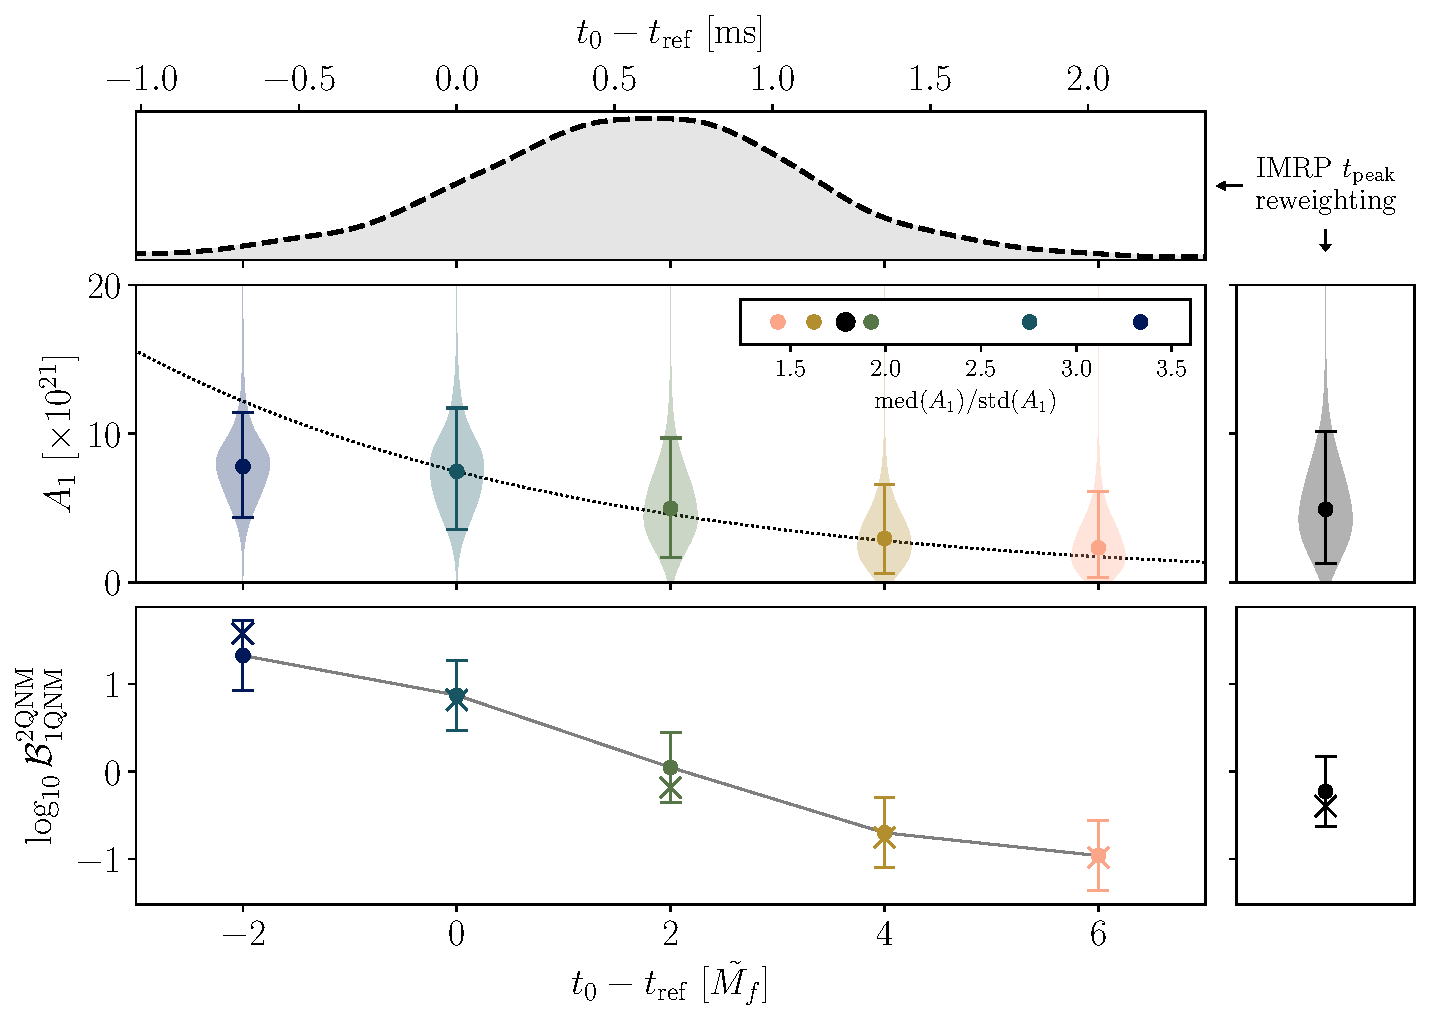
\includegraphics[width=0.9\columnwidth]{SearchingforaRingdownOvertoneinGW150914/overtone_amplitude_plot.pdf}
    \caption[Posteriors on the GW150914 overtone amplitude and Bayes' factors in favour of the overtone model for different choices of ringdown start time prior]{ 
    Posteriors on the overtone amplitude, and Bayes' factors in favour of the overtone model for different choices of $t_0$ prior (the colours and line styles correspond to those used in Fig.~\ref{fig:start_time}).
    \emph{Top:} posterior on the time of peak strain in the Hanford frame, from a \textsc{IMRPhenomPv2} analysis, as in Fig.~\ref{fig:start_time} (and originally from Ref.~\cite{Isi:2022mhy}). 
    \emph{Middle:} overtone amplitude posteriors for different choices of $t_0$ prior. The left panel corresponds to Gaussian priors with standard deviation $1\tilde{M_f}$, centred at the time they are plotted.
    The dotted line indicates the expected exponential decay of the $A_1$ mode; this is included merely to guide the eye and was produced using the median mass and spin values from the full IMR analysis and the median value of $A_1$ from the $\bar{t_0} = 0$ prior.
    The right panel corresponds to using the \textsc{IMRPhenomPv2} time of peak strain as a prior.
    For earlier start times the posteriors on the amplitude are peaked further away from zero; this is quantified in the inset plot where the ratio of the median to the standard deviation of the $A_1$ posterior is plotted.
    \emph{Bottom:} the Bayes' factor in favour of the overtone model for each prior choice; circles with error bars show the Bayes' factor calculated from nested sampling (with errors estimated by the sampler) while the crosses show the results calculated using the Savage-Dickey density ratio.    
    }
    \label{fig:overtone_amplitude}
\end{figure*}

Our results in Fig.~\ref{fig:mass_spin_post} can be compared to the corresponding results of the time-domain analyses shown in Fig.~1 from Cotesta et al.~\cite{Cotesta:2022pci} and Figs.~4 and 5 from Isi \& Farr~\cite{Isi:2022mhy}.
In general terms, there is broad agreement between all three sets of results. 
In particular, all three sets of authors find that the overtone analyses ($N=1$) always gives results that are more consistent with the IMR result and get increasingly broader for later choices of the ringdown start time.
All sets of authors also find that for the fundamental-only analysis ($N=0$) starting at early times (i.e.\ $t_0  - t_\mathrm{ref}\lesssim 0$) leads to posteriors that are inconsistent with the IMR result.
However, there are subtle differences between the various results.
Our results with $N=0$ and early start times gives posteriors biased to large values of $M_f$ and $\chi_f$; this is also seen in Ref.~\cite{Isi:2022mhy}, but not in Ref.~\cite{Cotesta:2022pci} (where the posterior consistently reaches lower values of $\chi_f$).
Our results with $N=0$ and late start times (i.e.\ $t_0 - t_\mathrm{ref}\gtrsim 4\tilde{M_f}$) are partially consistent with the IMR results; this is also seen in Ref.~\cite{Cotesta:2022pci}, but not in Ref.~\cite{Isi:2022mhy} who never find consistency with the IMR result for any choice of start time.
Finally, when including the overtone ($N=1$) and starting at late times, Ref.~\cite{Cotesta:2022pci} find results that are consistent with $\chi_f=0$ (i.e.\ a Schwarzschild BH) at 90\% confidence, in stark disagreement with Ref.~\cite{Isi:2022mhy} who find $\chi_f\gtrsim 0.2$. 
Our results are in better agreement with those of Ref.~\cite{Isi:2022mhy}.

In the middle panel of Fig.~\ref{fig:overtone_amplitude} we investigate our $N=1$ overtone analysis further by plotting the one-dimensional marginalised posteriors for the amplitude, $A_1$, of the QNM overtone.
An amplitude posterior peaked away from zero has been suggested (particularly by Ref.~\cite{Isi:2019aib}) as one good indication for the presence of an overtone in the data.
As expected, the QNM overtone decays quickly and when starting at later times we find a small value for the amplitude.
The degree to which the $A_1$ posterior is peaked away from zero can be quantified using the ratio between the median and standard deviation; this is plotted in the inset of the middle panel of Fig.~\ref{fig:overtone_amplitude}.
For values of $\bar{t_0}$ between $-2\tilde{M_f}$ and $+6\tilde{M_f}$, we find posteriors on $A_1$ that are peaked away from zero at between $1.44$ and $3.34\sigma$.
If we reweight using the IMRP $t_{\rm peak}$ prior, we find a posterior peaked away from zero at $1.79\sigma$.

Our results in the middle panel of Fig.~\ref{fig:overtone_amplitude} can be compared to the corresponding results of the time-domain analyses shown in Fig.~1 of Ref.~\cite{Isi:2022mhy} and Fig.~2 of Ref.~\cite{Cotesta:2022pci}.
All three sets of authors find values of $A_1$ that are smaller at later times, consistent with the expected exponential decay of the overtone, but they disagree on the absolute value of the amplitude and the significance with which a zero amplitude can be excluded.
Refs.~\cite{Isi:2019aib, Isi:2022mhy} find the largest values; they report a posterior peaked $3.6\sigma$ away from zero.
Ref.~\cite{Cotesta:2022pci} finds much smaller values which are consistent with zero for many choices of start time.
These analyses use essentially the same method and should therefore agree exactly.
Our result, produced using a different method, lies somewhere in between; we do find nonzero values are preferred for a range of start times, but only with a modest significance of $\sim 1.79\sigma$ for our preferred IMRP $t_{\rm peak}$ prior which we consider to be the best description of our uncertainty on the ringdown start time.

The comparison of our results with those of Refs.~\cite{Isi:2019aib, Cotesta:2022pci, Isi:2022mhy} is complicated by the fact that we use subtly different definitions for the amplitude. 
The time-domain analyses naturally define the mode amplitudes at a fixed time, usually $t_0$.
Our frequency-domain analysis also defines the mode amplitudes at $t_0$, but this start time is then varied as part of the analysis, blurring the exact time at which the amplitude is defined.
This is a fairly small effect for the narrow Gaussian priors, but more significant for the wider IMRP $t_{\rm peak}$ prior.
We can correct for this effect by rescaling all the overtone amplitudes to any fixed reference time (here we use $t_{\rm ref}$) using the known decay rate for the QNMs;
\begin{align}
	A_{1,\mathrm{ref}} = A_1 \exp\left(\frac{t_0-t_{\mathrm{ref}}}{\tau_{221}(M_f,\chi_f)}\right),
\end{align}
where $\tau_{221}(M_f, \chi_f)$ is the exponential decay time of the $(2,2,1)$ QNM and is a function of the remnant mass and spin.
This rescaling can be done for any QNM and the resulting amplitude parameters $A_{\ell m n,\mathrm{ref}}$ are more directly comparable with the amplitudes used in time-domain analyses.
Posteriors on $A_{1,\mathrm{ref}}$ are shown in  
Fig.~\ref{fig:amp_at_tref}.

\begin{figure}[t]
    \centering
    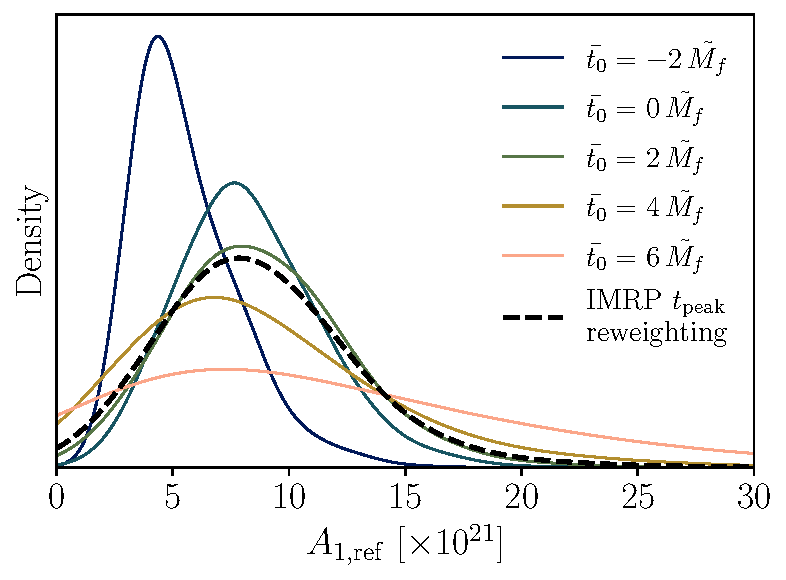
\includegraphics[width=0.6\columnwidth]{SearchingforaRingdownOvertoneinGW150914/overtone_amplitude_at_tref.pdf}
    \caption[Posteriors on the GW150914 overtone amplitude, rescaled to a fixed reference time]{ 
    Posteriors on the overtone amplitude from our $N=1$ overtone analysis, rescaled to a fixed reference time of $t_{\rm ref}$.
    The rescaling does not significantly affect the significance with which the posteriors are peaked away from zero.
    The colours and line styles indicate the prior used on $t_0$ and correspond to those used in Fig.~\ref{fig:start_time}.
    }
    \label{fig:amp_at_tref}
\end{figure}

In the bottom panel of Fig.~\ref{fig:overtone_amplitude} we plot the Bayes' factors between the fundamental only ($N=0$) and overtone ($N=1$) analyses.
This is defined as $\mathcal{B}_{\rm 1QNM}^{\rm 2QNM}=Z_{N=1}/Z_{N=0}$.
The Bayes' factor has been suggested (particularly by Ref.~\cite{Cotesta:2022pci}) as another good way for quantifying the support for an overtone in the data.
The Bayes' factor was computed in two different ways.
Firstly, \textsc{dynesty} was used to calculate the evidences $Z_{N=0}$ and $Z_{N=1}$ for both of the analyses described above, and these were reweighted to the desired $t_0$ prior using Eq.~\ref{eq:new_evidence}. 
Nested sampling also returns an estimate for the error on the evidences, and these are used to plot the error bars in Fig.~\ref{fig:overtone_amplitude}.
Secondly, exploiting the fact that the $N=0$ model is nested within the $N=1$ model, the Bayes' factors were computed using the posterior on $A_1$ from the $N=1$ analysis to find the Savage-Dickey density ratio~\cite{10.2307/2958475}. 

Our results in the bottom panel of Fig.~\ref{fig:overtone_amplitude} can be compared to the corresponding results of the time-domain analyses shown in Fig.~7 of Ref.~\cite{Isi:2022mhy} and Fig.~2 of Ref.~\cite{Cotesta:2022pci}.
Ref.~\cite{Cotesta:2022pci} computes the Bayes' factors using the ratio of evidences evaluated with nested sampling, whereas Ref.~\cite{Isi:2022mhy} computes Bayes' factors using Savage-Dickey density ratios.
All sets of authors find Bayes' factors that decrease for later ringdown start times, although they disagree on the exact value.
Ref.~\cite{Isi:2022mhy} finds the strongest log-evidence of $\sim 1.7$ at $t_0-t_{\rm ref} \sim 0$.
Ref.~\cite{Cotesta:2022pci} finds slightly negative log-evidence starting at this time.
Again, our result lies somewhere in between, we find a moderate log-evidence of $\sim 1.0$ when marginalising over a narrow prior on $t_0$ centred at this time.
If we instead marginalise over the time of peak strain using the broader IMRP $t_{\rm peak}$ prior, the evidence is slightly negative.
However, as discussed in Section~\ref{ch4:sec:discussion} below, we consider the actual values of the Bayes factors to be less important than their trend with varying start time.


\subsection{The nature of the overtone}\label{subsec:verify}

The results of the previous section show that there is tentative evidence for something beyond the fundamental $(2,2,0)$ mode in the GW150914 data. 
In the previous section it was assumed that this is the $(2,2,1)$ QNM overtone; this is motivated by our expectations from numerical relativity experiments (see, for example, Ref.~\cite{Giesler:2019uxc}). 
In this section, we address this assumption by measuring the frequency and amplitude of the QNM overtone and comparing with the expectations from GR.

Fig.~\ref{fig:delta_f} shows the results of a third ringdown analysis that also includes two QNMs.
In this analysis the complex frequency of the second QNM is allowed to deviate from the Kerr overtone value. 
This differs from the $N=1$ overtone analysis described above, where the frequency of the overtone was fixed by the remnant mass and spin to the Kerr value, $\omega_{221} = 2\pi f_{221} - i/\tau_{221}$.
Recovering a value of $\delta f$ consistent with zero has been suggested (particularly by Ref.~\cite{Isi:2022mhy}) as further evidence for the presence of an overtone; otherwise, it might be expected that the extra parameters would fit to the noise and would not recover the Kerr value.
We use the parameterisation from Ref.~\cite{Isi:2022mhy}; the complex frequency of the second QNM is now $\omega_{221} = 2\pi f-i/\tau$, where $f=f_{221}\exp(\delta f)$ and $\tau=\tau_{221}\exp(\delta \tau)$. 
This introduces the two new dimensionless parameters $\delta f$ and $\delta \tau$ into the model, for which we use uniform priors in the range $[-0.5,\, 0.5]$.
The $\delta \tau$ parameter is not well constrained, therefore we focus initially on $\delta f$.
We find posteriors on $\delta f$ consistent with zero for all choices of $t_0$ prior with standard deviations $\sim 0.2$. 
This is consistent with what was found in Ref.~\cite{Isi:2019aib} and can be viewed as a test of the no-hair theorem at the $\sim 20\%$ level.

\begin{figure}[t]
    \centering
    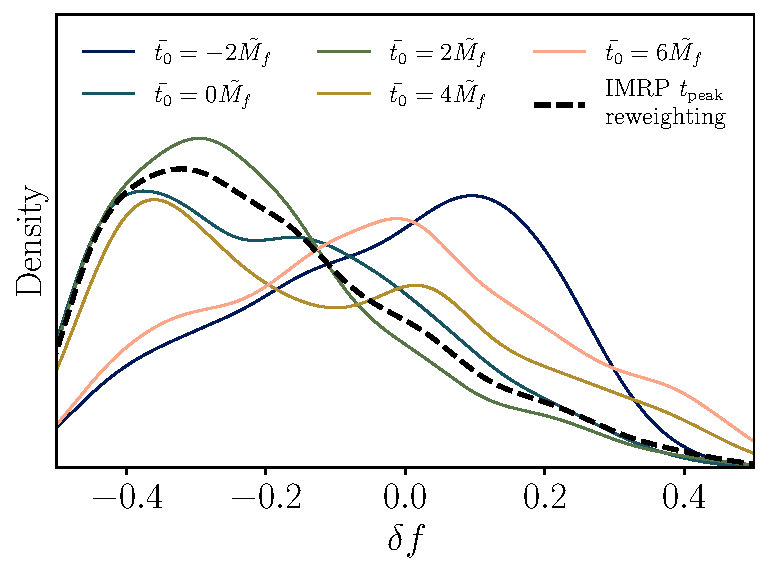
\includegraphics[width=0.6\columnwidth]{SearchingforaRingdownOvertoneinGW150914/220221_deviation_plot.pdf}
    \caption[Posteriors on the deviation from the Kerr for the real part of the GW150914 overtone frequency]{ 
    Posteriors on the deviation parameter from the Kerr value for the real part of the overtone frequency.
    The colours and line styles distinguish different choices for the $t_0$ prior and correspond to those used in Fig.~\ref{fig:start_time}.
    The mode frequency is given by $f_{221}^{\rm Kerr} \exp(\delta f)$, so that $\delta_f=0$ is the expected result for the Kerr metric.
    For all choices of $t_0$ prior the data is consistent with $\delta f=0$.
    }
    \label{fig:delta_f}
\end{figure}

Our results in Fig.~\ref{fig:delta_f} can be compared with Fig.~2 of Ref.~\cite{Isi:2022mhy}. 
Our preferred run, using the IMRP $t_{\rm peak}$ prior on $t_0$, is broadly consistent with that result.
However, what is notable about our results is that we do not find a significant broadening of the posterior for later choices of the start time. 
This was found by Ref.~\cite{Isi:2022mhy} and would be expected if an overtone was present, as both the overtone amplitude and ringdown SNR decaying with later ringdown start times.

\begin{figure}
    \centering
    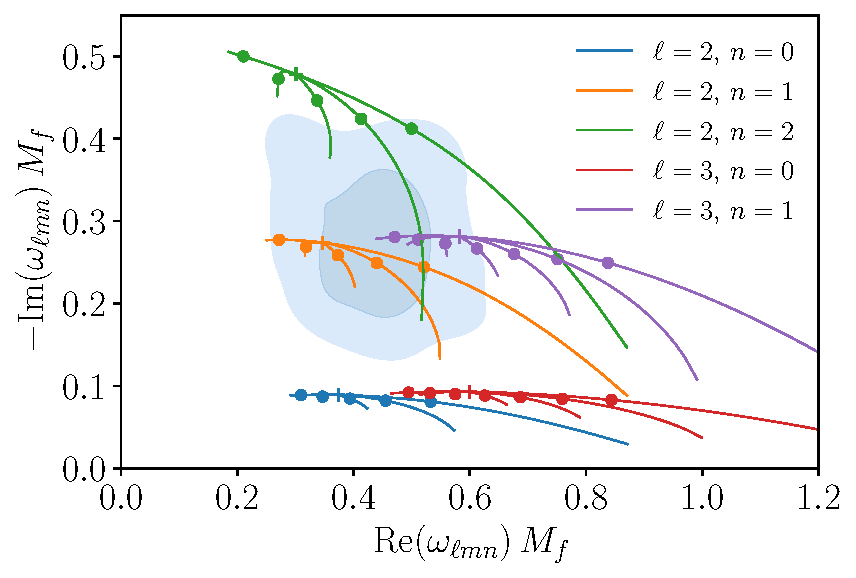
\includegraphics[width=0.6\columnwidth]{SearchingforaRingdownOvertoneinGW150914/kerr_spectrum_and_deviation.pdf}
    \caption[Posterior on the dimensionless complex frequency of the second GW150914 QNM assuming the first is the fundamental mode]{ 
    The posterior on the dimensionless complex frequency of the second QNM (50\% and 90\% regions), assuming the first is the fundamental $(\ell,|m|,n)=(2,2,0)$ mode.
    Lines indicate the Kerr frequencies parameterised by the remnant spin; dots and crosses indicate points with $\chi_f=0.7$ and $0$ respectively.
    Lines are coloured according to their $\ell$ and $n$ indices and the $m$ index increases left to right in each set.
    The frequency of the second QNM is consistent with the expected $(2,2,1)$ overtone, but also with several other modes.
    However, all fundamental modes (those with $n=0$) are excluded.
    }
    \label{fig:other_QNMs}
\end{figure}

\begin{figure}[t]
    \centering
    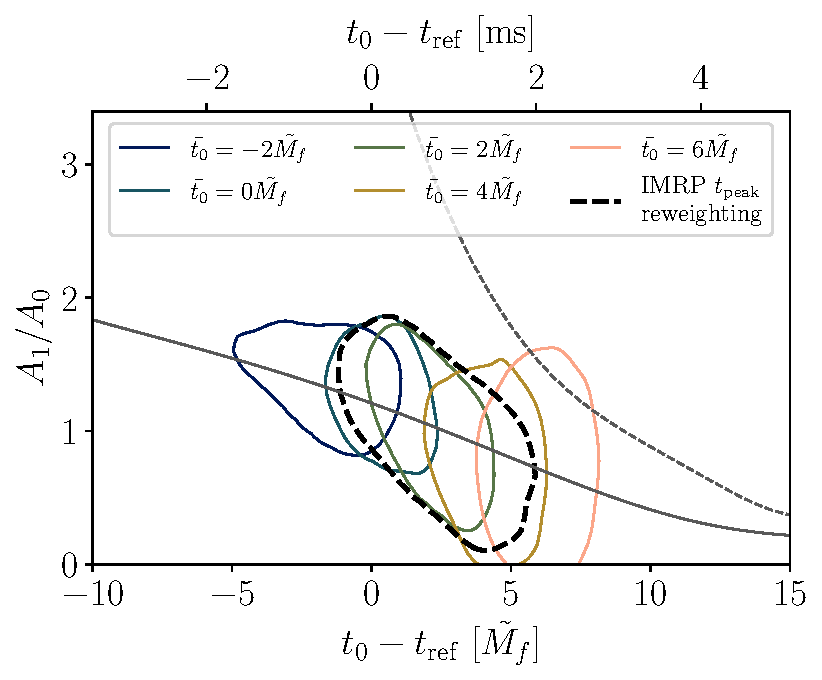
\includegraphics[width=0.6\columnwidth]{SearchingforaRingdownOvertoneinGW150914/amplitude_ratio.pdf}
    \caption[Posteriors on the amplitude ratio $A_1/A_0$ from the GW150914 overtone analysis]{ 
    Posteriors on the amplitude ratio $A_1/A_0$ from our $N=1$ overtone analysis. 
    The 90\% contours are plotted, with the colours and line styles indicating the $t_0$ prior and correspond to those used in Fig.~\ref{fig:start_time}.
    The solid grey curve shows the results of a two-QNM fit to the numerical relativity simulation SXS:BBH:0305 which has parameters consistent with GW150914.
    The dashed grey curve shows the results of a multi-QNM fit to SXS:BBH:0305 which follows closely the expected exponential decay rate for the amplitude ratio.
    }
    \label{fig:amp_ratio}
\end{figure}

To investigate this further, we use the results of the ringdown analysis where the frequency of the overtone is allowed to vary freely to address another important question. 
If the data does indeed contain a second QNM, can we determine which mode it is?
Theoretical studies of numerical relativity simulations suggest that the $(\ell,|m|,n)=(2,2,1)$ will be the next most prominent, especially for early start times~\cite{Giesler:2019uxc}. 
In Fig.~\ref{fig:other_QNMs} we plot the posterior on the dimensionless complex frequency (allowing both the real and imaginary parts to vary freely) of the second QNM, $\omega M_f$.
This plot uses the value for $M_f$ calculated from the complex frequency of the first QNM, assuming this is the expected $(2,2,0)$ fundamental mode of Kerr.
We find that we can confidently conclude that the second mode is an overtone ($n\geq 1$) but that it is not possible to say from the data alone exactly which overtone. 
For example, the modes $(2,2,1)$ and $(2,1,1)$ are both equally compatible with the data. 
In general, when searching for additional QNMs it is necessary to be guided by our prior expectations regarding which modes are expected to be excited with the highest amplitudes.

We now turn our attention to the measured amplitude $A_1$ and whether this matches the theoretical expectations for the $(2,2,1)$ overtone. 
For convenience, we choose to work with the amplitude ratio $A_1/A_0$ which eliminates factors common to all modes, such as the distance to the source. 
Because the two QNMs decay exponentially at different rates, the amplitude ratio depends strongly on the chosen ringdown start time.
Our two-dimensional posteriors on the amplitude ratio and ringdown start time are plotted in Fig.~\ref{fig:amp_ratio}.
As expected we find that the amplitude ratio decreases for later start times, and the error on the amplitude ratio increases for later start times because of the decreasing SNR in the ringdown.

In order to check whether this is consistent with the theoretical expectation for an overtone we compare with fits to the numerical relativity simulation SXS:BBH:0305~\cite{Lovelace:2016uwp} which has parameters consistent with GW150914.
Fixing the remnant mass and spin to the values reported in the simulation metadata, we perform QNM least-squares fits to this simulation for a range of ringdown start times using the code previously developed in Ref.~\cite{Finch:2021iip}.
Results are shown in Fig.~\ref{fig:amp_ratio} for two such fits. 
Firstly, we performed a two-QNM fit intended to mimic the analysis of the real GW150914 data described in Section~\ref{subsec:overtone} above. 
In this analysis the ${}_{-2}Y_{22}$ spherical harmonic mode of the simulation is modelled as a sum of the $(2,2,0)$ and $(2,2,1)$ QNMs and the amplitude ratio is recorded. 
The results from this two-QNM fit agree very well with what is seen in the real data giving us further confidence that there is nothing unexpected present in the data and that our results are not unduly affected by noise fluctuations (see also the discussion in Section~\ref{subsec:noise}). 
Secondly, we perform a full multi-QNM fit to all the spherical harmonic modes (up to and including $\ell = 8$) with a ringdown model that includes all QNMs (including both prograde and retrograde modes) up to $\ell = 8$ and $n = 7$ (1232 QNMs in total).
The ratio of the amplitudes of the $(2,2,0)$ and $(2,2,1)$ prograde modes from this fit behaves very differently; the ratio follows very closely a exponential time evolution which can be understood in terms of the difference between the two QNM decay times.

The fact that the two-QNM analysis gives a very different amplitude ratio compared to the full multi-QNM analysis for ringdown start times near the peak strain is related to the extreme destructive interference observed in the QNM overtone fits of Refs.~\cite{Giesler:2019uxc, Bhagwat:2019dtm, Ota:2019bzl, Cook:2020otn, JimenezForteza:2020cve, Dhani:2020nik, Finch:2021iip, Forteza:2021wfq, Dhani:2021vac, MaganaZertuche:2021syq} with large values of $N$.
This shows that the amplitude $A_1$ recovered from a two-QNM analysis is not purely the amplitude of the first overtone but also includes significant contributions from higher overtones and other harmonics. 
However, absorbing these contributions into the first overtone introduces a systematic bias in the remnant properties that is smaller than the statistical uncertainty; this can be seen in, for example, Fig.~\ref{fig:mass_spin_post} and Section IV\,C of Ref.~\cite{Giesler:2019uxc}. 
For this reason, it still makes sense to describe the results of the two-QNM analysis as a measurement of the overtone, even though there are undoubtedly other contributions present in the signal.


\subsection{The effect of noise and sampling frequency}\label{subsec:noise}

One of the key claims made in Ref.~\cite{Cotesta:2022pci} was the overtone detection was highly sensitive to noise fluctuations.
This was disputed by Ref.~\cite{Isi:2022mhy}.
In order to address this issue, we performed a noise injection study mirroring closely what was done in Ref.~\cite{Cotesta:2022pci}.
The results of this injection study are presented in Section~\ref{app:inj}.
As expected, the results of injecting into different noise realisations show some scatter.
However, this scatter is not larger than expected and we are unable to reproduce the claim in Ref.~\cite{Cotesta:2022pci} with our (very different) analysis method. 

It has been suggested~\cite{WillMaxTGRtelecon} that the results of ringdown analyses, in particular those including overtones, might be sensitive to aliasing effects when using downsampled strain data due to the reduced Nyquist frequency.
QNM overtones, $(\ell, m, n \geq 1)$, have roughly the same real part of the frequency as the corresponding fundamental, $(\ell, m, 0)$, mode, but they have a shorter damping time. 
See, for example, Fig.~\ref{fig:other_QNMs}. 
This means that if a single, isolated, mode is viewed in Fourier space, the power spectrum is broader and contains significant power at higher frequencies.

Early ringdown studies, including those in Refs.~\cite{LIGOScientific:2016lio, Isi:2019aib, Isi:2022mhy}, generally used strain data that had been downsampled to $2\,$kHz. 
This was done for convenience and computational speed and was not originally anticipated to be a problem because the merger of GW150914 occurs at $\sim 200\,\mathrm{Hz}$, safely below the Nyquist frequency.

In this chapter the $4\,$kHz data is used for all the analyses in the main text. 
Additionally, a frequency-domain log-likelihood with an upper integration limit of $f_{\rm high}=1000\,$Hz was used.
Our method is very different from the time-domain analyses, and do not expect our results to be sensitive to small changes in these choices.
To check that this is the case we have repeated the $N=1$ overtone analysis using the $16\,$kHz sampled data (obtained from Ref.~\cite{gwosc}) and we find no significant changes in our results.
Using reweighting techniques (this time applied to the likelihood) we have also investigated the effect of changing the upper limit of integration in the likelihood. 
By re-evaluating the $N=1$ posterior chain on a likelihood with $f_\mathrm{high}=1500\,$Hz and $2000\,$Hz, and then reweighting, we again find no significant changes in our results.


\subsection{Posteriors on the ringdown start time}\label{app:t0_posterior_prior}

As described in Section~\ref{subsec:reweighting}, we initially perform Bayesian inference on the ringdown using a broad, flat prior on the ringdown start time parameter $t_0$. 
The posteriors on $t_0$ from both the $N=0$ and $N=1$ analyses are shown in Fig.~\ref{fig:t0_posterior}.
We do not consider these posteriors to be physically meaningful results because they were obtained with a prior that does not correctly describe our state of knowledge about when the ringdown should start.
These results are produced merely as an intermediate step in our analysis, before the reweighting was applied, and are shown here only to further illustrate the reweighting procedure described in Section~\ref{subsec:reweighting}.

\begin{figure}[b!]
    \centering
    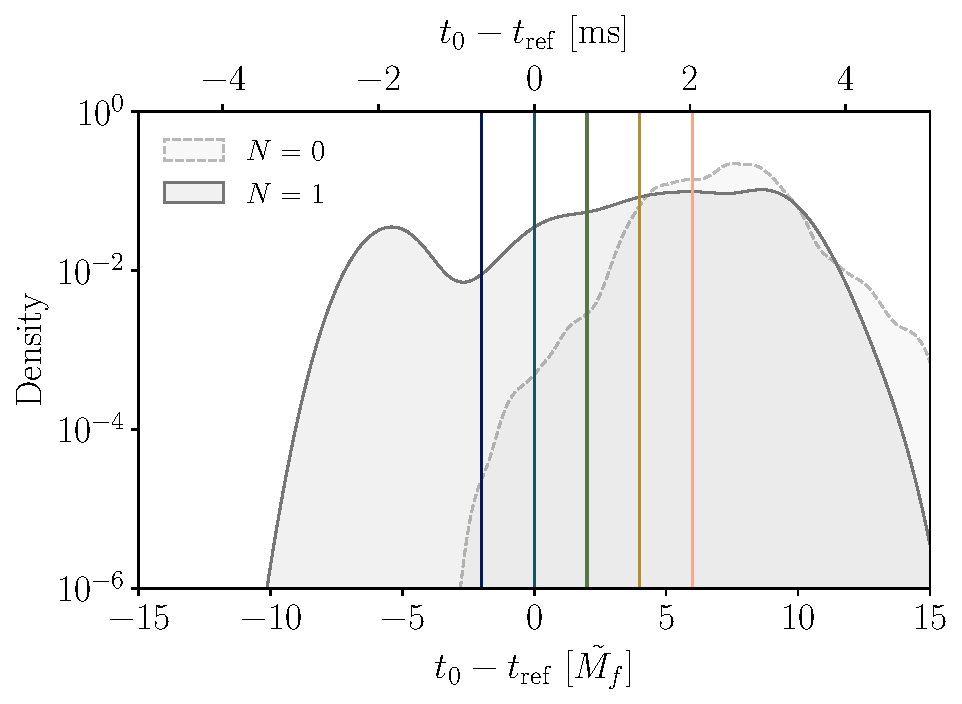
\includegraphics[width=0.6\columnwidth]{SearchingforaRingdownOvertoneinGW150914/unweighted_t0_posteriors.pdf}
    \caption[Posteriors on the GW150914 ringdown start time]{ 
    Posteriors on the ringdown start time obtained from our initial analysis using a flat prior over the range shown in the plot.
    Results are shown for the fundamental only ($N=0$) and overtone ($N=1$) analyses.
    Vertical coloured lines show the locations of the means $\bar{t_0}$ of the narrow Gaussian priors used for the subsequent reweighting (see Fig.~\ref{fig:start_time}).
    The $N=1$ posterior has ample support across the entire range of interest, as required for the reweighting to remain accurate.
    The $N=0$ posterior has enough support everywhere except the $\bar{t_0}=-2\ \tilde{M_f}$ prior.
    }
    \label{fig:t0_posterior}
\end{figure}

In order for the subsequent reweighting step to be accurate, it is necessary for the posterior chains (particularly for the $N=1$ overtone analysis) to contain samples across the range of start times that we consider. 
For this reason, the \textsc{dynesty} sampler settings described in Section~\ref{sec:details} were chosen to ensure a large number of posterior samples were produced; we obtained 203697 and 218882 posterior samples from the $N=0$ and $N=1$ analyses respectively. 
This is sufficient for the reweighting to remain accurate everywhere except for the earliest start time in the $N=0$ analysis. 
This is the reason why this result is omitted from Fig.~\ref{fig:mass_spin_post}.


\subsection{Injection study}\label{app:inj}

Closely following the injection study performed in Ref.~\cite{Cotesta:2022pci}, we inject GW150914-like signals in the instrumental noise surrounding the true GW150914 event and reperform our overtone analysis ($N=1$).

The $\ell=2$ spin-weighted spherical harmonic of the numerical relativity simulation SXS:BBH:0305~\cite{Lovelace:2016uwp} was used as the mock signal, scaled to a total mass of $72\,M_\odot$ and injected with a face-off orientation at a luminosity distance of $410\,\mathrm{Mpc}$. 
The sky position was taken to be $\alpha = 1.95\,\mathrm{rad}$, $\delta=-1.27\,\mathrm{rad}$.
This signal was injected into the data surrounding GW150914, such that the peak of the absolute value of the strain occurred at times $[-20, -15, -10, 5, 15, 20, 25, 30, 35, 40]\,\mathrm{s}$ relative to $t_\mathrm{ref}$.
These choices ensure the mock signal does not overlap with the real event.
Additionally, a zero-noise injection was performed for comparison. 

\begin{figure}[t]
    \centering
    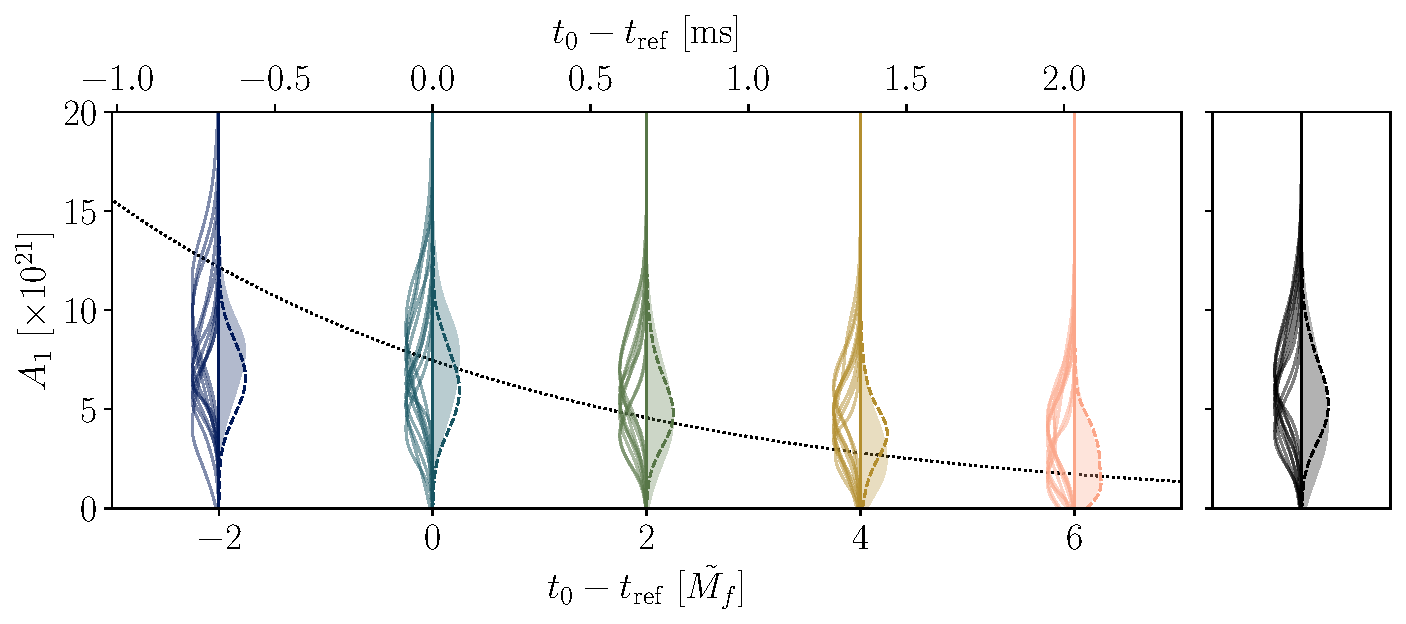
\includegraphics[width=0.9\columnwidth]{SearchingforaRingdownOvertoneinGW150914/injection_study_amps_only.pdf}
    \caption[Posteriors on the overtone amplitude from a noise injection study]{ 
    This is similar to the middle panel of Fig.~\ref{fig:overtone_amplitude} in the main text, but shows the posteriors on the overtone amplitude from the noise injection study.
    The different violin plots are for the different priors on the ringdown start time and the colours are the same as those used in Figs.~\ref{fig:start_time} and \ref{fig:overtone_amplitude}.
    On the right-hand side of each set of violin plots, the filled posterior shows the result obtained using the real GW150914 data (this is the same as what is plotted in Fig.~\ref{fig:overtone_amplitude}). 
    On the left-hand side are all the posteriors from the injection campaign, which indicate the spread in results due to different noise realisations.  
    Finally, the dashed lines on the right-hand side are the posteriors from the zero-noise injection.
    This plot is intended to be compared to Fig.~2 of Ref.~\cite{Cotesta:2022pci}, and Fig.~6 of Ref.~\cite{Isi:2022mhy}.
    }
    \label{fig:injection_study}
\end{figure}

We performed the frequency-domain ringdown analysis on these mock datasets using the same setup as was used for the real data and as described in Section~\ref{sec:details}.
This includes using the same PSD in the likelihood for all datasets.
We plot the resulting posteriors on the overtone amplitudes in Fig.~\ref{fig:injection_study}.
As with the real data, prior reweighting (see Section~\ref{subsec:reweighting}) has been used to show results for different choices of the ringdown start time prior.
We also investigated the Bayes' factors and found the same declining trend.

As expected, different noise realisations introduce some scatter into the results and we observe a spread in the locations of the maximum posterior values for the overtone amplitudes. 
However, this spread is consistent with the width of the posterior. 
The analysis described in the main text found only tentative evidence for the overtone, but there is no indication that this is overly effected by noise fluctuations.


\subsection{Wavelet posteriors}\label{app:W3}

The frequency-domain ringdown analysis method described in Chapter~\ref{Chapter3} and used here marginalises over the early-time inspiral-merger signal using a flexible combination of sine-Gaussian wavelets (see Eq.~\ref{eq:wavelets}).
In the GW150914 analyses presented in this chapter $W=3$ wavelets were used.
This choice was found empirically to be large enough to model the inspiral-merger signal without biasing the ringdown inference.
We have also verified that no strong correlations are observed between the wavelet and QNM parameters, and that further increasing the number of wavelets does not significantly affect the results for physically meaningful parameters (such as remnant parameters $M_f$ and $\chi_f$). 
These tests are described further in Section~\ref{app:GW150914}.

The whitened strain posterior on the sum of these wavelets, together with the QNMs, can be seen in the early-time signal in Fig.~\ref{fig:waveform} where the fit to the data is seen to be excellent.
The wavelet parameters themselves are not physical; the wavelets are being used here solely to marginalise out the inspiral-merger. 
Nevertheless, in this section we show some additional posterior plots on the wavelet parameters, see Fig.~\ref{fig:wavelet}.
As expected, in order to describe the ``chirping'' inspiral signal, the wavelets naturally order themselves with their amplitudes and frequencies increasing with time. 

\begin{figure}[t]
    \centering
    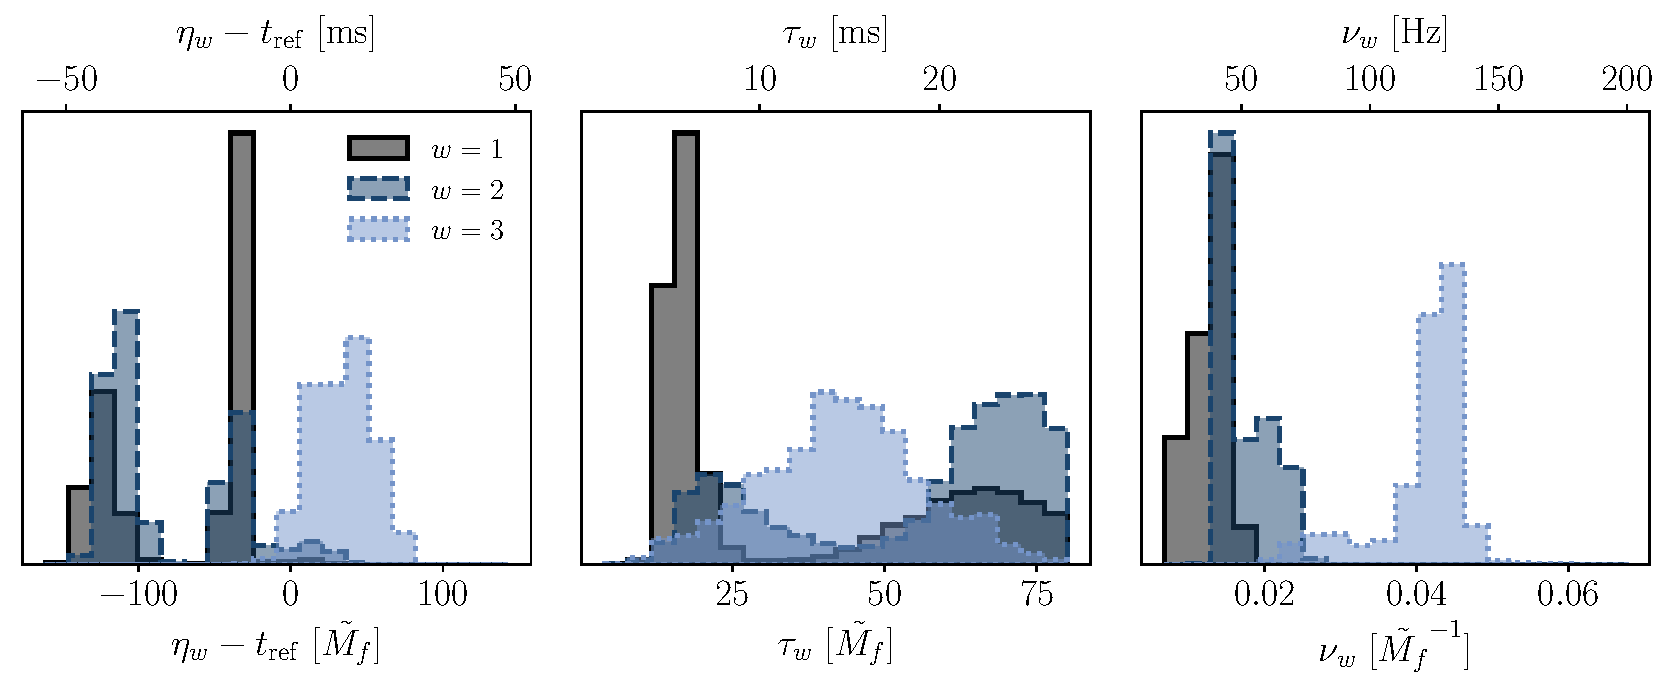
\includegraphics[width=0.9\columnwidth]{SearchingforaRingdownOvertoneinGW150914/wavelet_posterior_figure.pdf}
    \caption[Posteriors on selected wavelet parameters used in the GW150914 overtone analysis]{ 
    Posteriors on selected parameters for the $W=3$ wavelets used in the $N=1$ overtone analysis, reweighted using the IMRP $t_{\rm peak}$ prior on the ringdown start time.
    \emph{Left:} the wavelet central times, $\eta_w$.
    \emph{Middle:} the wavelet widths, $\tau_w$.
    \emph{Right:} the wavelet frequencies, $\nu_w$. 
    The index runs over values $w=1,\,2$ and $3$, where the numbering of the wavelets is chosen to enforce the ordering $\nu_{w}<\nu_{w+1}$.
    All plots use SI units on the upper $x$-axis and natural units on the lower $x$-axis. 
    }
    \label{fig:wavelet}
\end{figure}



\subsection{Other results}\label{subsec:other_results}

\begin{figure}[b!]
    \centering
    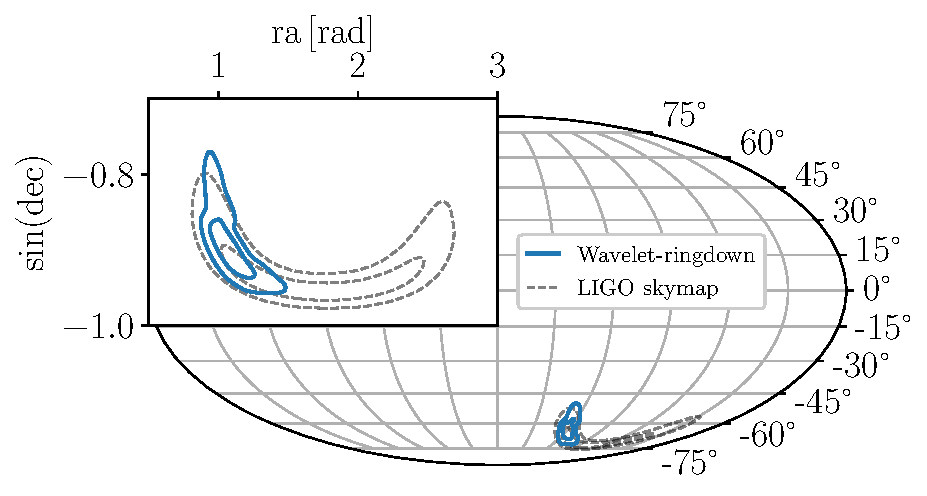
\includegraphics[width=0.9\columnwidth]{SearchingforaRingdownOvertoneinGW150914/skymap.pdf}
    \caption[Posterior on the GW150914 source sky position]{ 
    Posterior on the source sky position using geocentric coordinates in Mollweide projection.
    Shown in blue is the results from the $N=1$ overtone analysis using the IMRP $t_{\rm peak}$ reweighting for the prior on the ringdown start time.
    The LIGO skymap for this event is shown by the dashed black line for comparison.
    The inset plot shows a zoomed-in map plotted using right ascension and the sine of the declination.
    In both cases, 50\% and 90\% contours are plotted.
    }
    \label{fig:skymap}
\end{figure}

One important benefit of the frequency-domain approach to ringdown data analysis introduced in Chapter~\ref{Chapter3} and used here is that it naturally allows us to search (and hence to numerically marginalise) over source sky position and ringdown start time. 
This should be contrasted with the treatment of these parameters in most time-domain analyses where these parameters are fixed, potentially biasing the results. (Although it is technically possible to search over the sky in a time-domain analysis~\cite{Carullo:2019flw, Isi:2021iql}, this is rarely done in practice.)
To emphasise this, we plot the posterior on the sky location of GW150914 from our $N=1$ overtone analysis reweighted to the IMRP $t_{\rm peak}$ prior on the ringdown start time.
This can be compared with the publicly available LIGO sky posterior for GW150914 obtained using the samples from Ref.~\cite{skysamples}.
This is shown in Fig.~\ref{fig:skymap}.
As discussed in Chapter~\ref{Chapter3} (see the discussion around Fig.~\ref{fig:t0_geocent_posterior}), it should be emphasised that this sky posterior is not a ringdown-only result because much of the information is also coming from the wavelets used to model the inspiral-merger portion of the signal.

\begin{figure}[t]
    \centering
    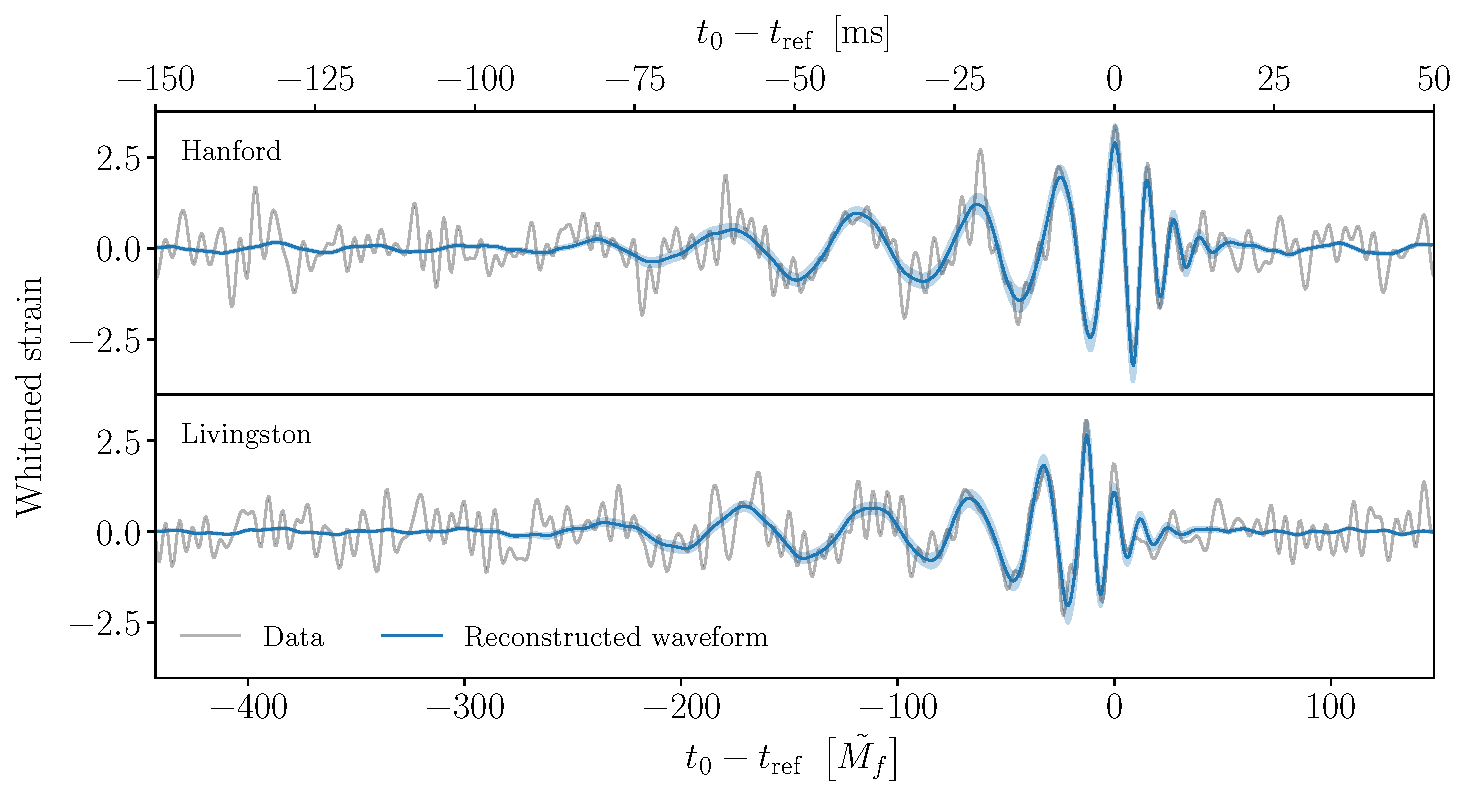
\includegraphics[width=0.9\columnwidth]{SearchingforaRingdownOvertoneinGW150914/waveform_plot.pdf}
    \caption[Posterior on the GW150914 reconstructed whitened waveform]{ 
    Posterior on the reconstructed whitened waveform.
    Shown in grey is the strain data from both LIGO interferometers (\emph{top}: Hanford, \emph{bottom}: Livingston) whitened according to the noise amplitude spectral density in the detector and bandpass filtered between 32 and $512\,\mathrm{Hz}$ for clarity.
    Shown in blue is the waveform reconstruction from the $N=1$ overtone analysis with the IMRP $t_{\rm peak}$ reweighting for the prior on the ringdown start time.
    The blue lines and shaded regions indicate median and the 90\% credible interval. 
    The signal is plotted as a function of time from $t_{\rm ref}$ using both SI and natural units on the upper and lower $x$-axis respectively.
    }
    \label{fig:waveform}
\end{figure}

Because the inspiral and merger parts of the signal are being modelled using truncated wavelets as part of the frequency-domain ringdown analysis, this allows us to plot a full waveform reconstruction from our results.
This reconstruction is shown in Fig.~\ref{fig:waveform} for our $N=1$ overtone analysis reweighted to the IMRP $t_{\rm peak}$ prior.
The full waveform model used in our analysis is discontinuous at $t_0$. However, as discussed in Chapter~\ref{Chapter3}, the whitened waveform reconstruction plotted here is smooth; this is a result of marginalising over the location of the discontinuity at $t_0$, the waveform model ``learning'' the continuity from the data, and the whitening process used to make the figure.
This waveform reconstruction uses the posterior on all of the model parameters, including those for the wavelets; more details on these parameters are given in Section~\ref{app:W3}.


\section{Conclusions}\label{ch4:sec:discussion}

The main motivation for this work comes from the ongoing discussion in the literature about whether a ringdown overtone can be confidently detected in the GW150914 data. 
In particular, the detection claim made in Ref.~\cite{Isi:2019aib} was disputed by Ref.~\cite{Cotesta:2022pci} where a nearly identical time-domain analysis was reperformed (see also the reply Ref.~\cite{Isi:2022mhy}).
Applying the frequency-domain ringdown analysis originally presented in Chapter~\ref{Chapter3}, we contribute to this discussion with a thorough reanalysis of the GW150914 data. 
This includes performing analyses with and without an overtone while considering different ringdown start times, as well as performing a noise injection study and studying the effects of different data sampling rates and frequency integration limits on our results.
Although the method used here differs significantly from previous time-domain analyses, we present our results in a way that makes it as easy as possible to compare with earlier work.
In conclusion, we do find tentative evidence for a ringdown overtone, but not at the high level of significance originally claimed in Ref.~\cite{Isi:2019aib}.

In order to be more quantitative, it is first necessary to be able to say clearly what it even means to ``detect a overtone''. 
Although intuitively obvious, it is not clear how to make this notion precise (this issue has previously been discussed in Ref.~\cite{Isi:2022mhy}). 
Several approaches have been suggested: looking to see if including the overtone improves the posterior on the remnant parameters (see Fig.~\ref{fig:mass_spin_post}); looking at the posterior on the overtone amplitude for a range of start times (see middle panel of Fig.~\ref{fig:overtone_amplitude}); computing the Bayes' factor in favour of an overtone (see bottom panel of Fig.~\ref{fig:overtone_amplitude}); and allowing the frequency of the second QNM to vary freely to see if the data prefers, or at least is consistent with, the expected Kerr value (see Figs.~\ref{fig:delta_f} and \ref{fig:other_QNMs}).
Although these are not all independent from one another, they all help shed light on which QNMs are present. 
The results of all of these tests can also be compared to results from a noise injection study.

As well as not being completely independent of each other, none of these tests are, by themselves, sufficient to justify a claim of a detection.
For example, one issue that has been raised is that the Bayes' factor can be made to take any value with a suitable adjustment to the prior range.
There are also conceptual problems regarding what it means to compare two models, neither of which is expected to fully describe the data. Here we are comparing the fundamental-only mode model (with a single QNM) to the overtone model (with two QNMs) when our firm prior belief is that the true signal should contain an infinite number of QNMs plus additional corrections (e.g.\ from nonlinearities in the merger, tails, and memory effects).

From the above discussion, it is clear that ringdown analyses are rather subtle. 
We think our frequency-domain method has some important advantages over what has been done before. 
For example, it marginalises over the ringdown start time and sky position which is preferable to fixing these parameters (which potentially introduces systematic biases). 
Ideally, we should also marginalise over the uncertainties in the noise power spectral density (see, e.g.,\ Ref.~\cite{Cornish:2020dwh}) and detector calibration (see, e.g.,\ Ref.~\cite{LIGOScientific:2017aaj}) as part of a ringdown analysis. 
The ability to do this is, in principle, another benefit of the frequency-domain analysis approach used here as this can be done using techniques that are standard in the field.

We stress that while our results have been compared with those of previous time-domain studies, our frequency-domain method is rather different and therefore we do not expect to find perfect agreement. 
In contrast, the results of Refs.~\cite{Isi:2019aib, Cotesta:2022pci, Isi:2022mhy} are produced using essentially identical methods and should therefore be expected to agree exactly. 
The reason for the disagreement that is seen there is currently unknown and the subject of an ongoing investigation by both sets of authors.
It is vitally important for QNM science that all results are reproducible. To that end we have made all our data products and plotting scripts publicly available at Ref.~\cite{finch_eliot_2022_6949492}.

If QNMs are going to fulfill their promise for testing GR, fundamental physics and the Kerr metric hypothesis, then the community must be able to agree on standards for what it means to detect them and to be able to robustly quantify their significance. 
This field is still very young, and that there is already significant controversy regarding the QNM content of GW150914 and GW190521 is concerning, and we risk the situation becoming more confused with many more suitable events expected in O4.
And, as discussed in the introduction, this is a conceptual issue that will not be resolved with more observations, even at higher SNRs.
This issue needs input from the whole community; however, we suggest that (as a minimum) future claims of an overtone detection are accompanied by the investigations in Fig.~\ref{fig:mass_spin_post}, both panels of Fig.~\ref{fig:overtone_amplitude} and Fig.~\ref{fig:delta_f}.
That is, posteriors on the remnant properties with and without the overtone, posteriors on the overtone amplitude, a study of the Bayes' factor trends for different start times, and posteriors on deviations from Kerr when the overtone frequency is allowed to vary.

All data products and plot scripts associated with this work are made publicly available at Ref.~\cite{finch_eliot_2022_6949492}.
 
%\include{Chapters/Chapter5} 

%----------------------------------------------------------------------------------------
%	THESIS CONTENT - APPENDICES
%----------------------------------------------------------------------------------------

\appendix % Cue to tell LaTeX that the following "chapters" are Appendices

% Include the appendices of the thesis as separate files from the Appendices folder
% Uncomment the lines as you write the Appendices

% Appendix A

\chapter{Frequently Asked Questions} % Main appendix title

\label{AppendixA} % For referencing this appendix elsewhere, use \ref{AppendixA}

\section{How do I change the colors of links?}

The color of links can be changed to your liking using:

{\small\verb!\hypersetup{urlcolor=red}!}, or

{\small\verb!\hypersetup{citecolor=green}!}, or

{\small\verb!\hypersetup{allcolor=blue}!}.

\noindent If you want to completely hide the links, you can use:

{\small\verb!\hypersetup{allcolors=.}!}, or even better: 

{\small\verb!\hypersetup{hidelinks}!}.

\noindent If you want to have obvious links in the PDF but not the printed text, use:

{\small\verb!\hypersetup{colorlinks=false}!}.

%\include{Appendices/AppendixB}
%\include{Appendices/AppendixC}

%----------------------------------------------------------------------------------------
%	BIBLIOGRAPHY
%----------------------------------------------------------------------------------------

\singlespacing
\printbibliography

%----------------------------------------------------------------------------------------

\end{document}  

